\documentclass[conference]{IEEEtran}

\usepackage{amsmath}
\usepackage{graphicx}

\title{Serial and OpenMP Parallel Implementation of a Three-Dimensional DEM Solver}
\author{\IEEEauthorblockN{Praveen Kumar Jha}
\IEEEauthorblockA{HPSC 2026\\
Assignment 1}}

\begin{document}
\maketitle

\begin{abstract}
This work presents a three-dimensional discrete element method (DEM) solver for spherical particles inside a rectangular box. The implementation computes translational motion only and uses a linear spring-dashpot normal-contact model for particle-particle and particle-wall interactions. A serial C++ baseline was developed first, followed by verification tests, runtime profiling, and OpenMP-based parallelisation of the particle-contact stage. Two optional extensions were also completed: a cell-based neighbour-search method and scientific studies on damping, and particle-cloud settling. Results show that the pair-contact loop dominates runtime in the baseline code, OpenMP provides useful acceleration on multi-core runs, and the neighbour-search method greatly reduces candidate-pair counts for larger particle systems.
\end{abstract}

\begin{IEEEkeywords}
DEM, OpenMP, particle simulation, neighbour search, parallel performance
\end{IEEEkeywords}

\section{Introduction}
The objective of this assignment was to construct, verify, and parallelise a simple three-dimensional DEM solver. I followed the workflow suggested in the assignment itself: first writing a serial solver, then checking it on simple test cases, then profiling it, and finally parallelising the expensive part of the code with OpenMP. The solver was written in C++ and set up to write CSV files so that the same runs could be reused for plotting and analysis. This report covers the main assignment and the optional bonus tasks up to Section 19. The larger research extension from Section 20 was not attempted here.

\section{Mathematical Formulation}
Each particle is represented by its position $\mathbf{x}_i$, velocity $\mathbf{v}_i$, mass $m_i$, and radius $R_i$. The translational motion is governed by Newton's second law,
\begin{equation}
    m_i \frac{d\mathbf{v}_i}{dt} = \mathbf{F}_i,
\end{equation}
with
\begin{equation}
    \frac{d\mathbf{x}_i}{dt} = \mathbf{v}_i.
\end{equation}
The total force on particle $i$ is the sum of gravity, particle-contact forces, and wall-contact forces. For particles $i$ and $j$, the overlap is
\begin{equation}
    \delta_{ij} = R_i + R_j - \|\mathbf{x}_j - \mathbf{x}_i\|.
\end{equation}
When $\delta_{ij} > 0$, the normal contact force is
\begin{equation}
    \mathbf{F}_{ij}^c = F_n \mathbf{n}_{ij}, \qquad
    F_n = \max(0, k_n \delta_{ij} - \gamma_n v_{n,ij}),
\end{equation}
where $\mathbf{n}_{ij}$ is the particle-particle unit normal and $v_{n,ij}$ is the relative normal velocity. Wall contacts use the same spring-dashpot form with wall normals defined by the box boundaries.

\section{Numerical Algorithm}
Time advancement uses the semi-implicit Euler scheme,
\begin{align}
    \mathbf{v}_i^{n+1} &= \mathbf{v}_i^n + \frac{\mathbf{F}_i^n}{m_i}\Delta t, \\
    \mathbf{x}_i^{n+1} &= \mathbf{x}_i^n + \mathbf{v}_i^{n+1}\Delta t.
\end{align}
At each timestep the code performs the following operations:
\begin{enumerate}
\item zero particle forces,
\item add gravity,
\item evaluate particle-particle contacts,
\item evaluate wall contacts,
\item integrate velocity and position,
\item compute diagnostics and write selected output.
\end{enumerate}

Here, ``diagnostics'' means the summary quantities that are calculated from the particle state at each saved timestep, such as total kinetic energy, maximum speed, center-of-mass position, active-contact count, candidate-pair count, and maximum particle height. These quantities are written to CSV files and later used for verification, profiling, and plotting.

The implementation is modular, with separate functions for contact evaluation, wall handling, diagnostics, profiling, and experiment drivers. This made it easier to test small pieces of the code and also made debugging simpler when verification runs did not initially behave as expected.

\section{Verification and Testing}
Three verification studies were performed before moving on to performance work.

\subsection{Free Fall}
A single particle was released from rest with gravity acting in the negative $z$ direction. The numerical trajectory was compared against the analytical solution
\begin{equation}
    z(t) = z_0 - \frac{1}{2}gt^2.
\end{equation}
For this verification case the run was stopped before the particle reached the floor, so the analytical free-fall curve remained valid over the full plotted interval. Figure~\ref{fig:freefall} shows close agreement between the numerical and analytical trajectories. In addition, Figure~\ref{fig:freefallvel} compares the numerical and analytical vertical speed magnitude, which confirms that the solver reproduces both the correct position and the correct acceleration-driven velocity change. The two curves remain visually indistinguishable over most of the plotted interval, which indicates that the force assembly and the semi-implicit Euler update are both behaving consistently in this simple one-particle limit.

\begin{figure}[t]
    \centering
    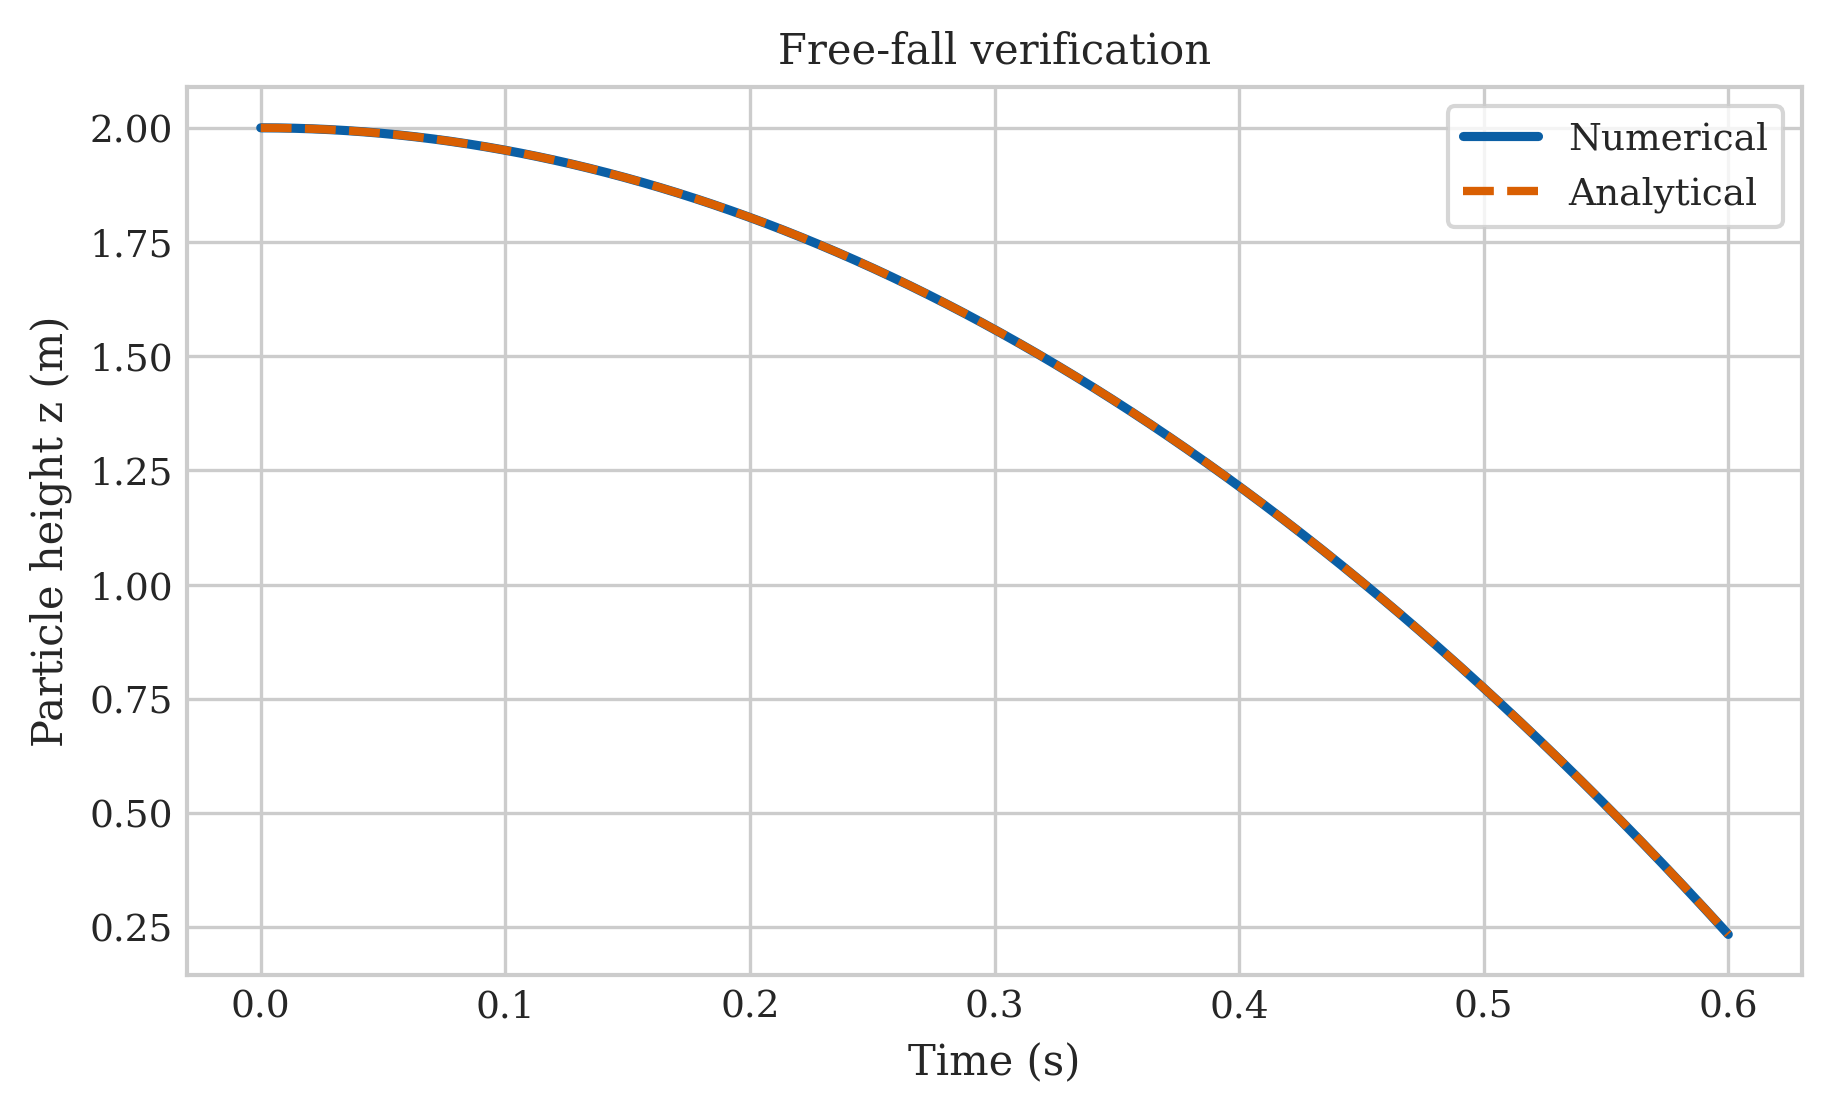
\includegraphics[width=\columnwidth]{figures/free_fall_numerical_vs_analytical.png}
    \caption{Free-fall verification comparing numerical and analytical height histories.}
    \label{fig:freefall}
\end{figure}

\begin{figure}[t]
    \centering
    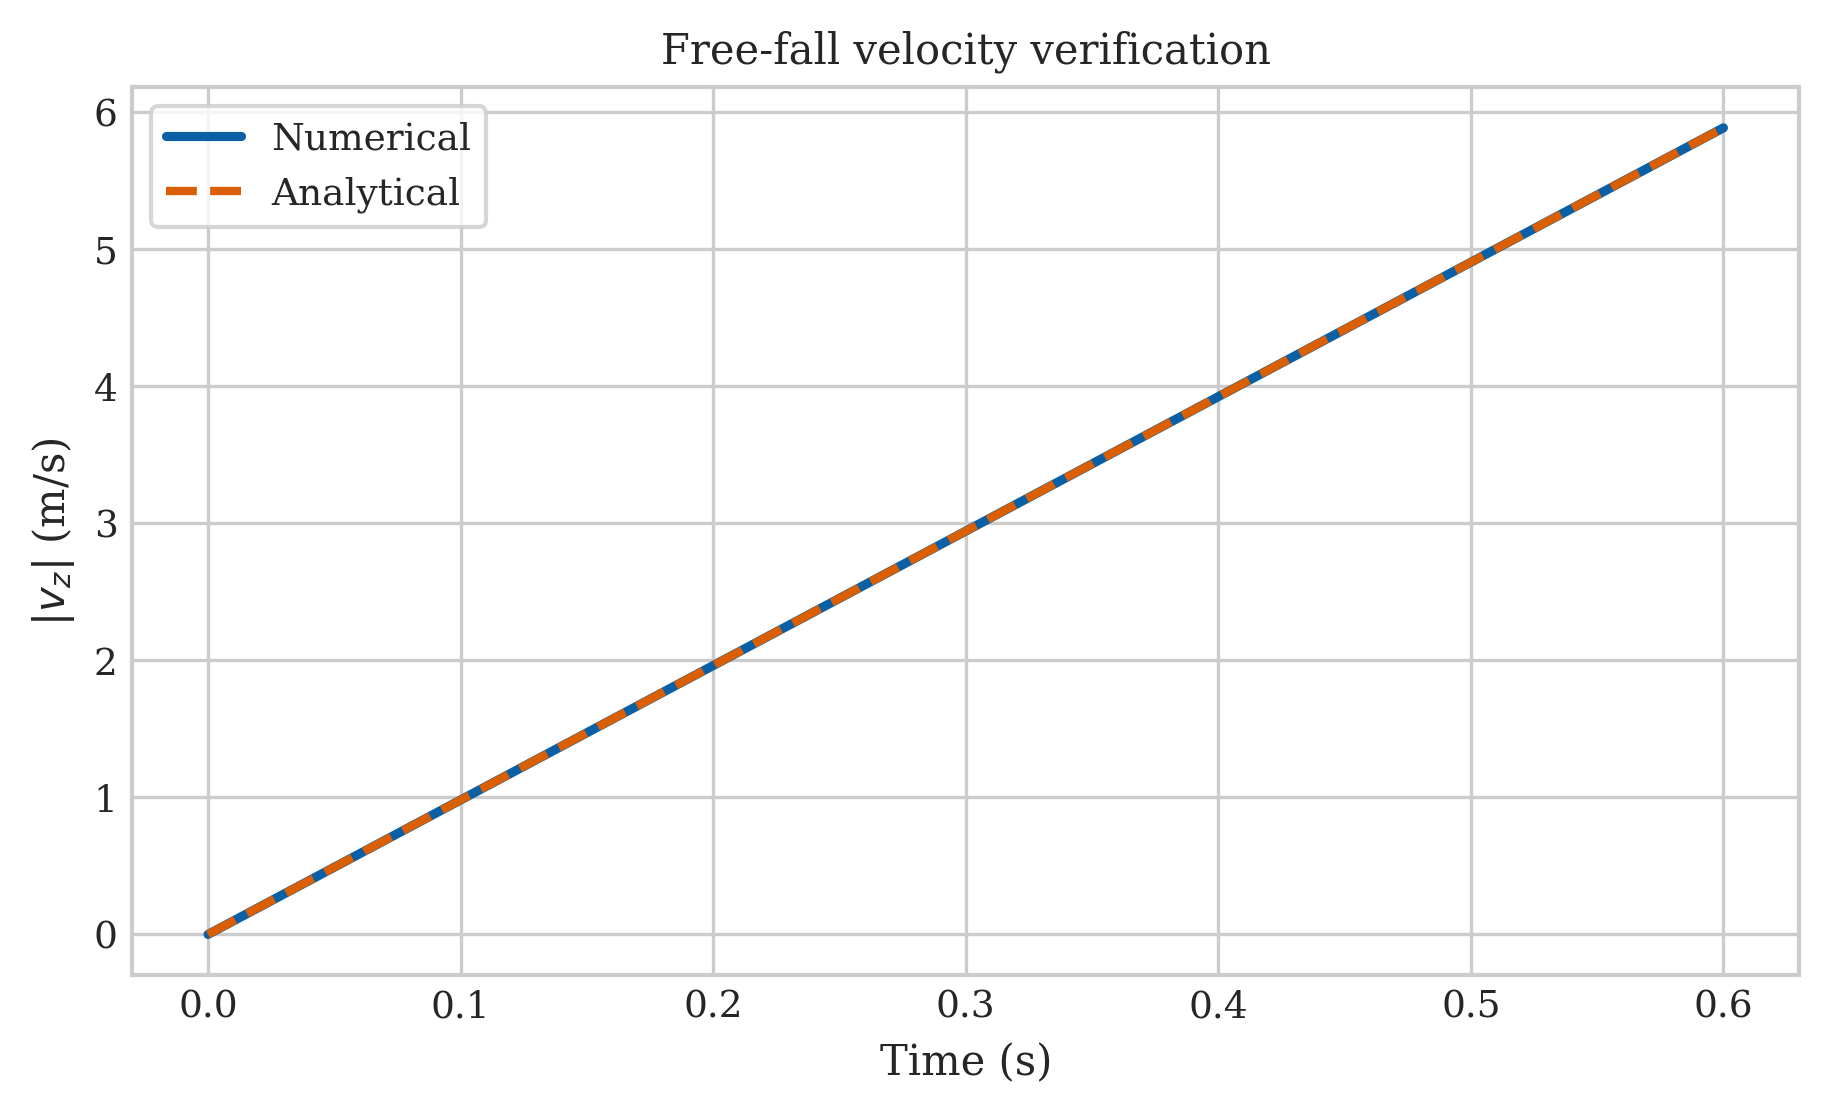
\includegraphics[width=\columnwidth]{figures/free_fall_velocity_numerical_vs_analytical.png}
    \caption{Free-fall verification comparing numerical and analytical vertical speed magnitude.}
    \label{fig:freefallvel}
\end{figure}

The assignment also asks for an error-versus-timestep study. This was carried out by repeating the free-fall case for several values of $\Delta t$ and recording the final height error at the end of the run. Figure~\ref{fig:dtstudy} shows that this error decreases as the timestep is refined, which is the expected behaviour for the present time-integration scheme. The trend is monotone over the tested range, so the figure gives a direct practical guideline as well: smaller timesteps improve accuracy, but they do so at the cost of additional timesteps and higher runtime.

\begin{figure}[t]
    \centering
    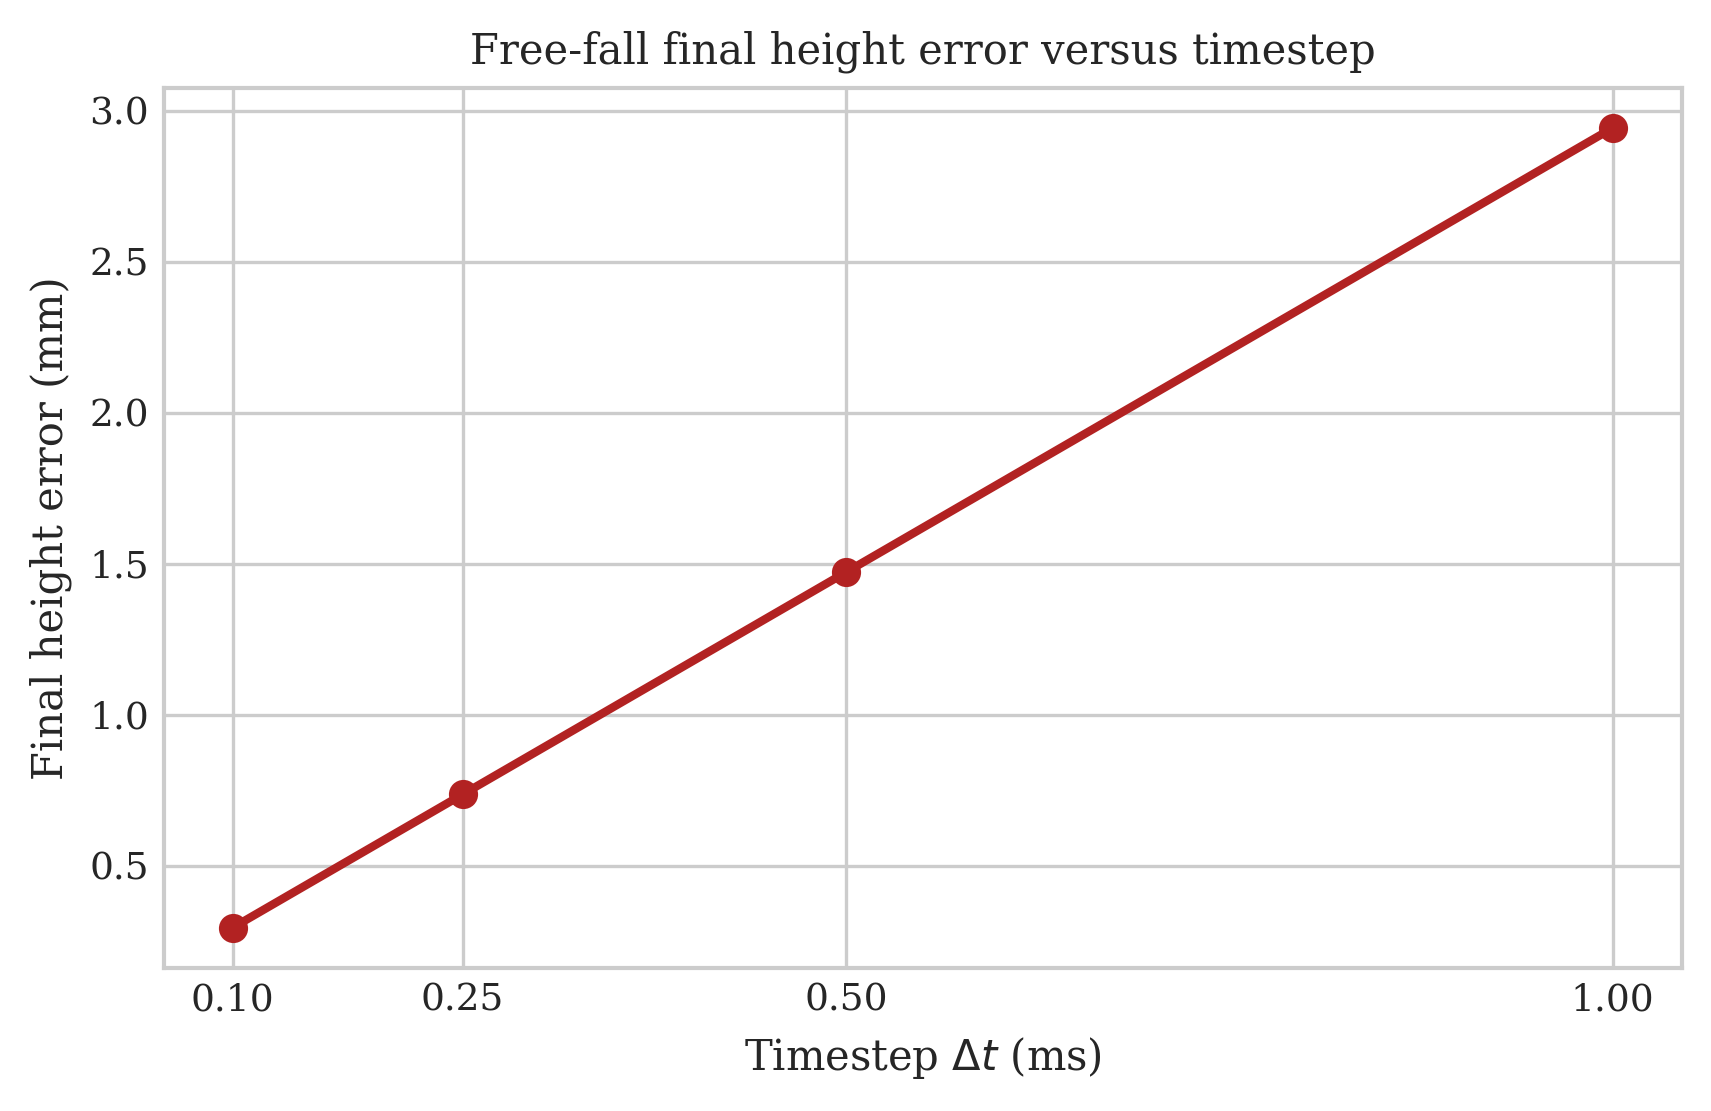
\includegraphics[width=\columnwidth]{figures/timestep_sensitivity.png}
    \caption{Final free-fall height error as a function of timestep size.}
    \label{fig:dtstudy}
\end{figure}

\subsection{Constant Velocity}
Gravity was disabled and a single particle was initialised with a non-zero velocity. In this case the exact solution is a straight-line trajectory with constant velocity. The verification was therefore checked in two ways: by comparing the numerical and analytical positions in each coordinate direction, and by confirming that the numerical velocity components remained constant in time. Figure~\ref{fig:cvtraj} shows the position comparison and Figure~\ref{fig:cvvel} shows the velocity comparison. Together these results confirm that the zero-force case is being integrated correctly. In particular, the velocity curves remain flat, which shows that no spurious acceleration is introduced when the contact and gravity terms are inactive.

\begin{figure}[t]
    \centering
    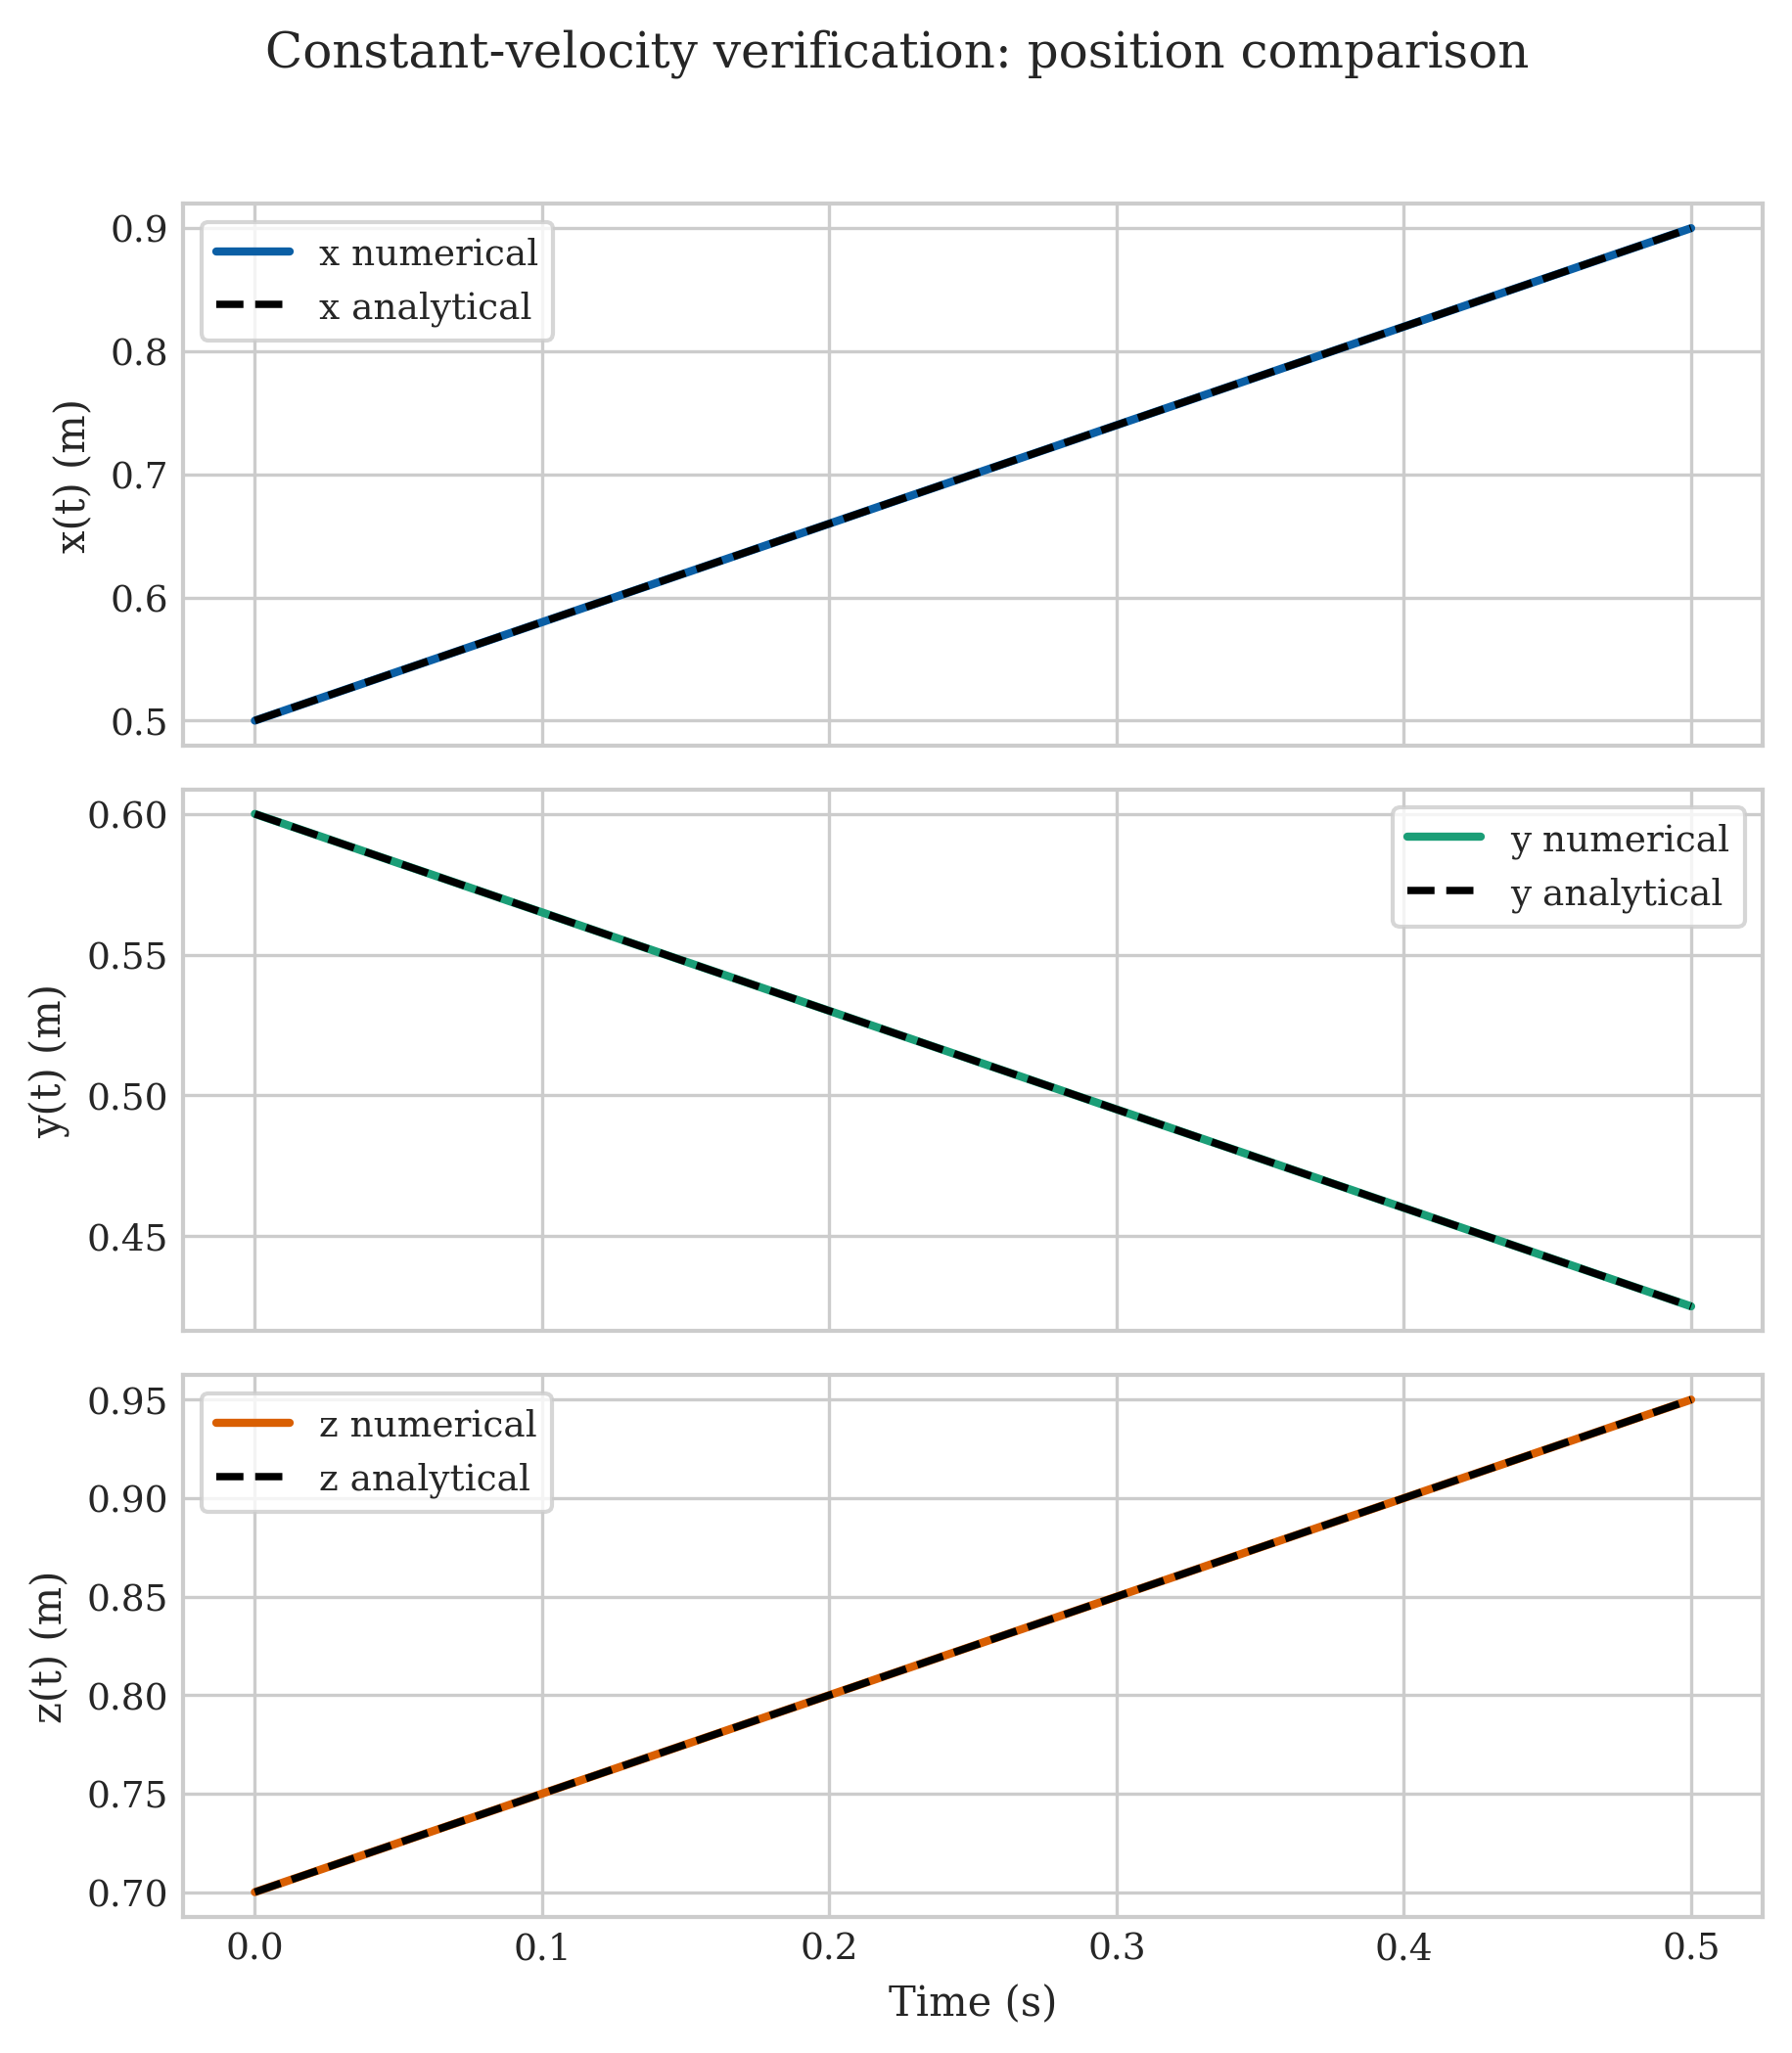
\includegraphics[width=\columnwidth]{figures/constant_velocity_numerical_vs_analytical.png}
    \caption{Constant-velocity verification comparing numerical and analytical motion.}
    \label{fig:cvtraj}
\end{figure}

\begin{figure}[t]
    \centering
    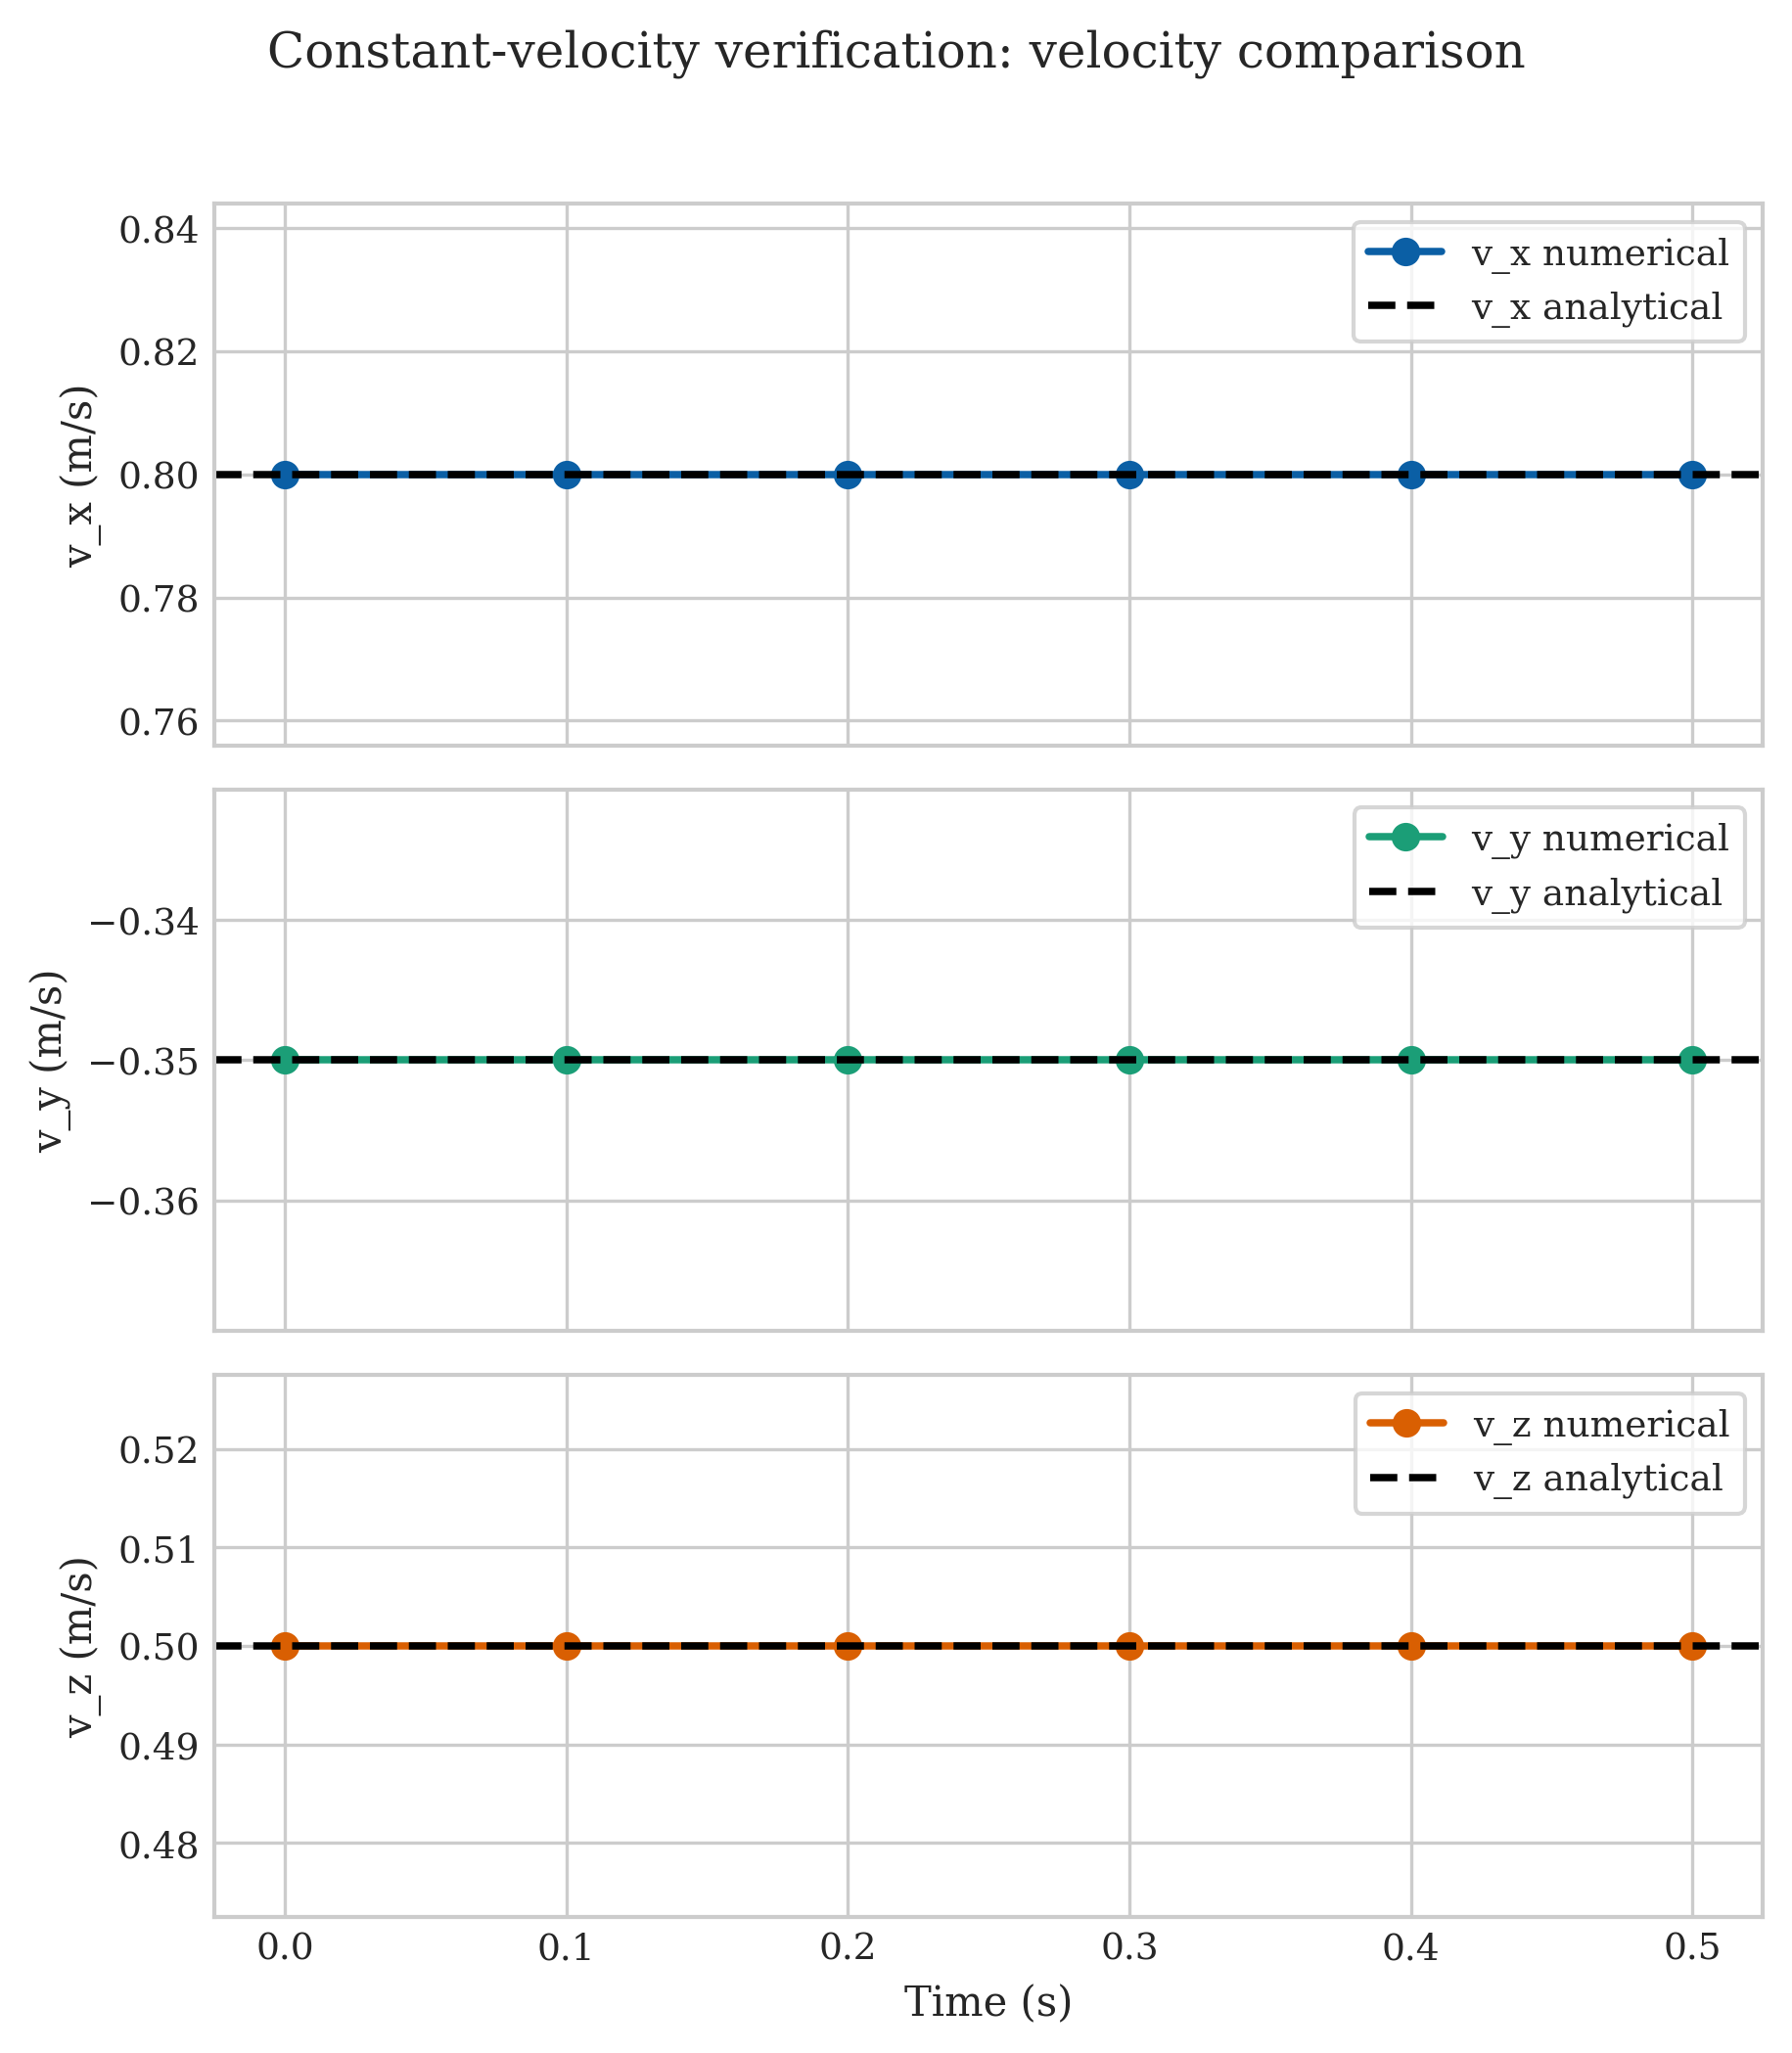
\includegraphics[width=\columnwidth]{figures/constant_velocity_velocity_check.png}
    \caption{Constant-velocity verification comparing numerical and analytical velocity components.}
    \label{fig:cvvel}
\end{figure}

\subsection{Bounce Test}
A particle was dropped onto the lower wall. This test was used to check that the wall-contact model behaves physically: the particle should rebound after impact, wall penetration should remain bounded, and stronger damping should reduce the rebound response. Figure~\ref{fig:bounce} compares the height history for light and heavy damping, Figure~\ref{fig:bounceke} shows the corresponding kinetic-energy history, and Figure~\ref{fig:penetration} shows the wall overlap. The wall overlap remains small in both cases, so the particle does not penetrate excessively. In addition, the heavier damping case shows a clearly reduced rebound height and a faster decay of kinetic energy, which matches the expected qualitative behaviour. The sharp drops in kinetic energy correspond to dissipative wall impacts: the particle gains kinetic energy during free fall, then loses part of it rapidly at contact, and the retained amount becomes smaller when the damping coefficient is increased.

\begin{figure}[t]
    \centering
    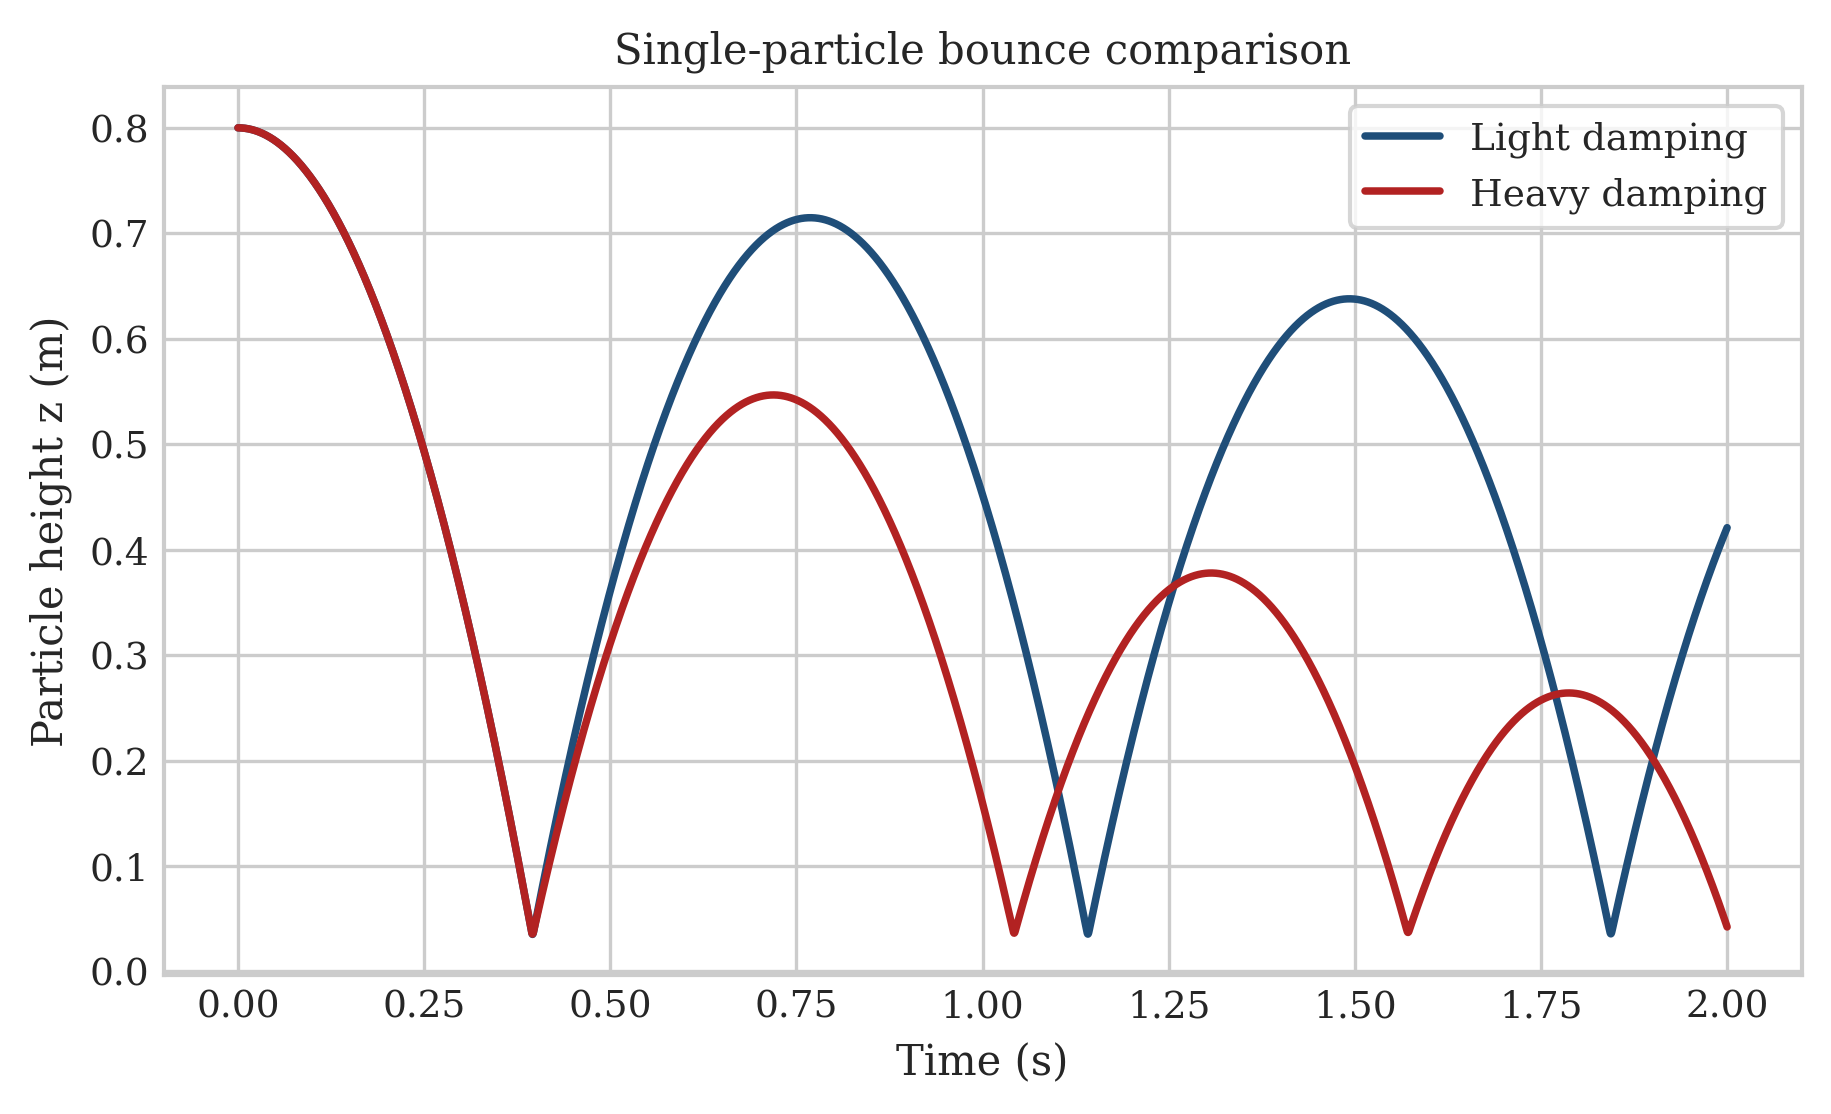
\includegraphics[width=\columnwidth]{figures/bounce_height_vs_time.png}
    \caption{Bouncing-particle height history used for wall-contact verification.}
    \label{fig:bounce}
\end{figure}

\begin{figure}[t]
    \centering
    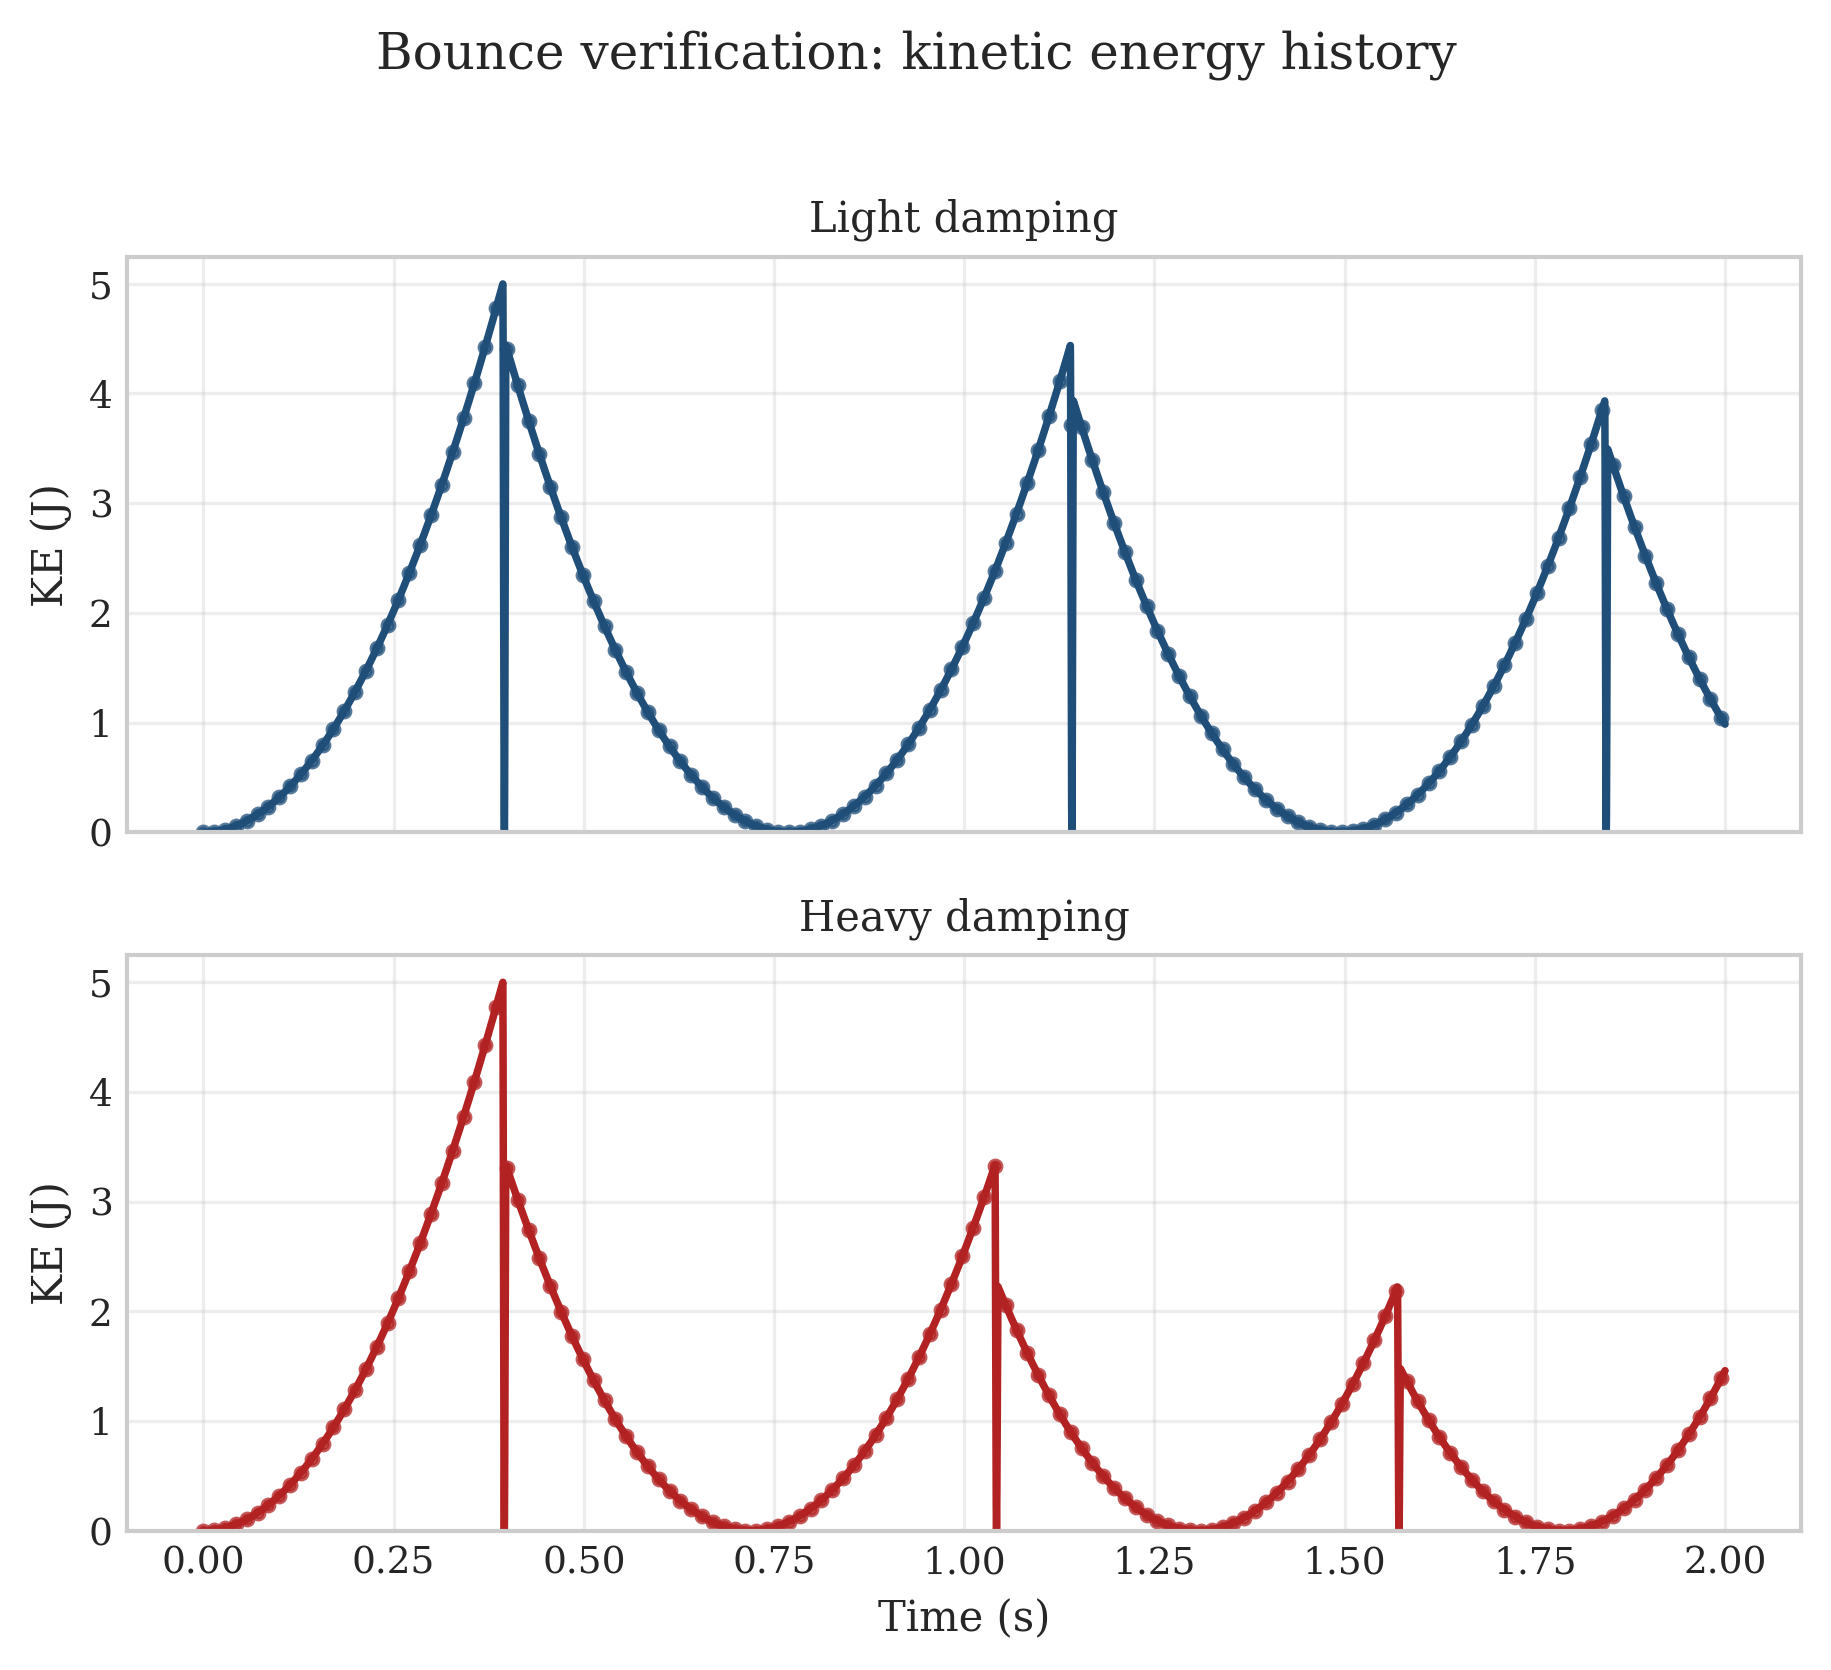
\includegraphics[width=\columnwidth]{figures/bounce_kinetic_energy_vs_time.png}
    \caption{Kinetic-energy history during the bounce verification case.}
    \label{fig:bounceke}
\end{figure}

\begin{figure}[t]
    \centering
    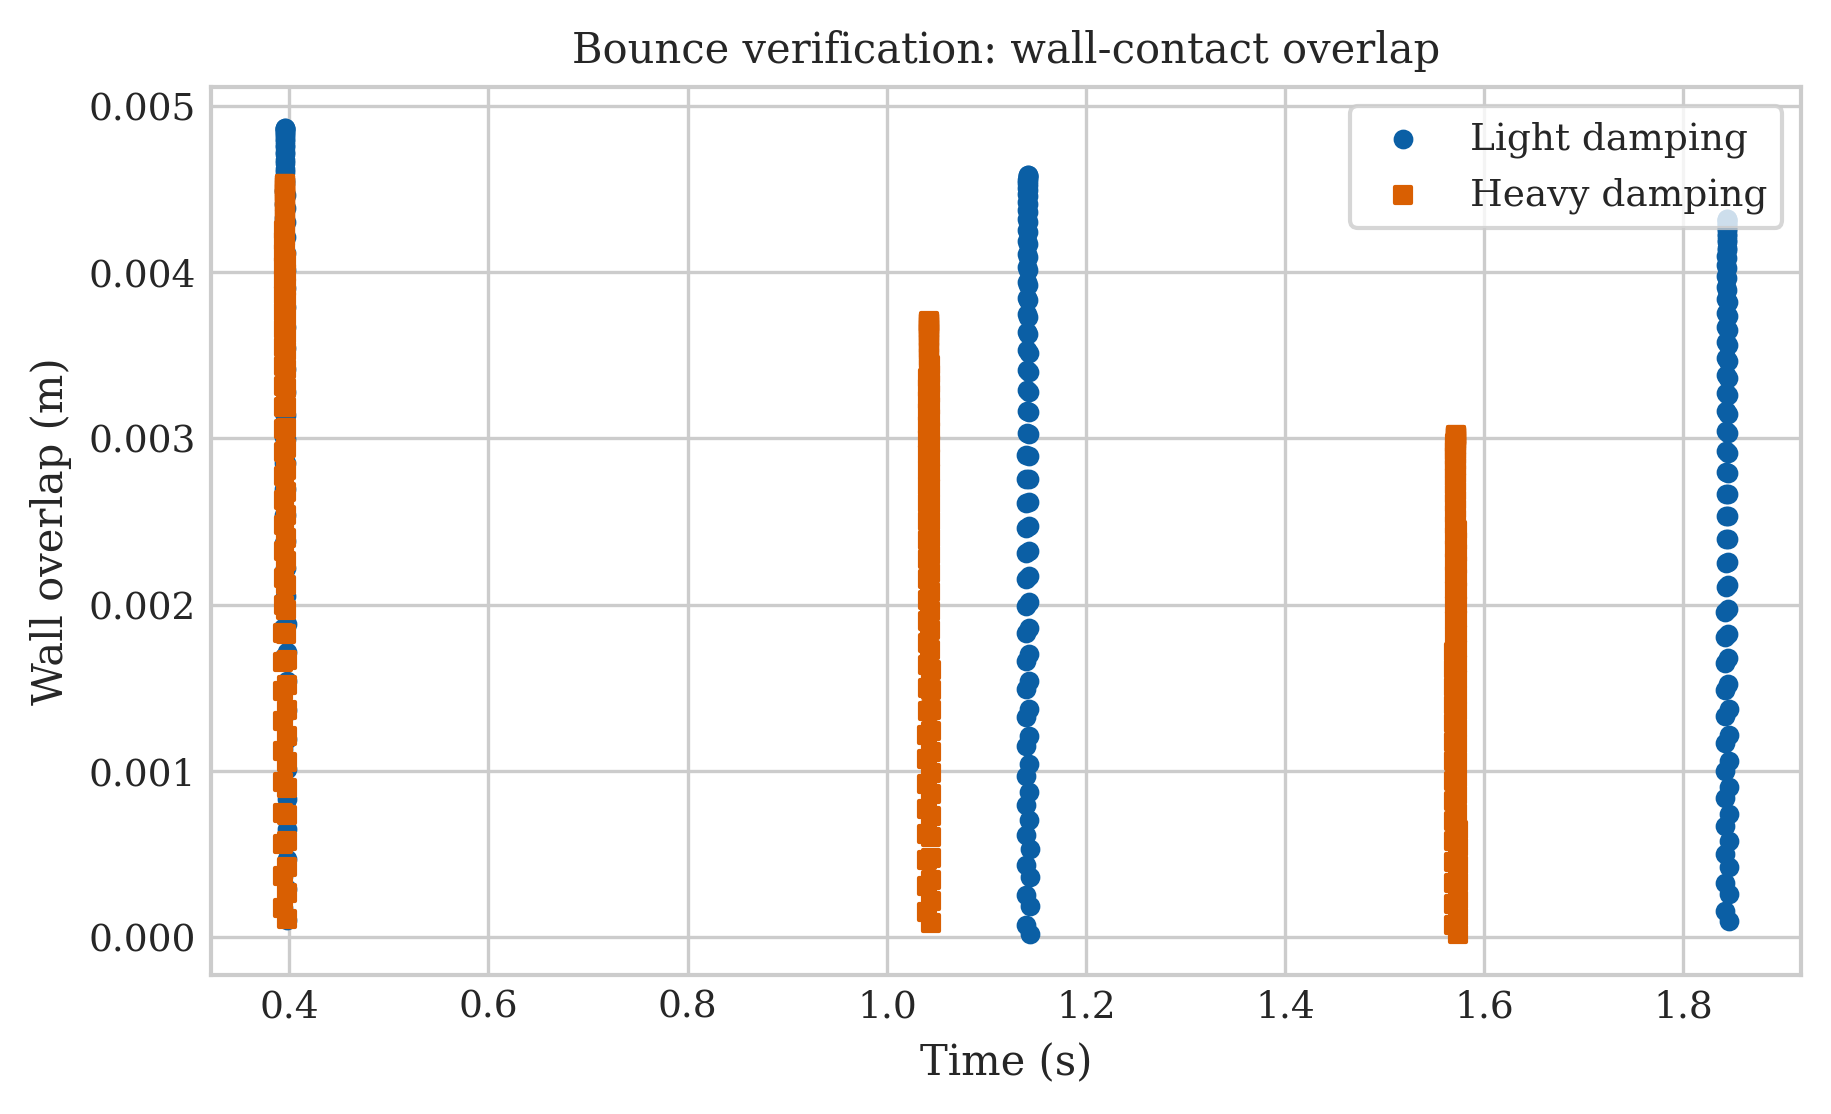
\includegraphics[width=\columnwidth]{figures/bounce_wall_overlap.png}
    \caption{Wall overlap during the bounce verification case. The overlap remains bounded, indicating that the particle does not penetrate excessively.}
    \label{fig:penetration}
\end{figure}

\section{Simulation Experiments}
After verifying the one-particle cases, the solver was run for systems with increasing particle counts: $N=200$, $1000$, and $5000$. These runs were used to study how the computational cost and the basic system response change as the number of particles increases.

Figure~\ref{fig:particle_runtime} shows that the runtime grows rapidly with particle count, and that the particle-contact stage dominates the total runtime more strongly as $N$ becomes larger. This is expected because the baseline serial implementation uses brute-force all-pairs contact checking. The total-runtime curve and the dashed contact-stage curve lie very close to one another for the larger cases, which is itself evidence that most of the wall-clock time is being spent in contact evaluation.

\begin{figure}[t]
    \centering
    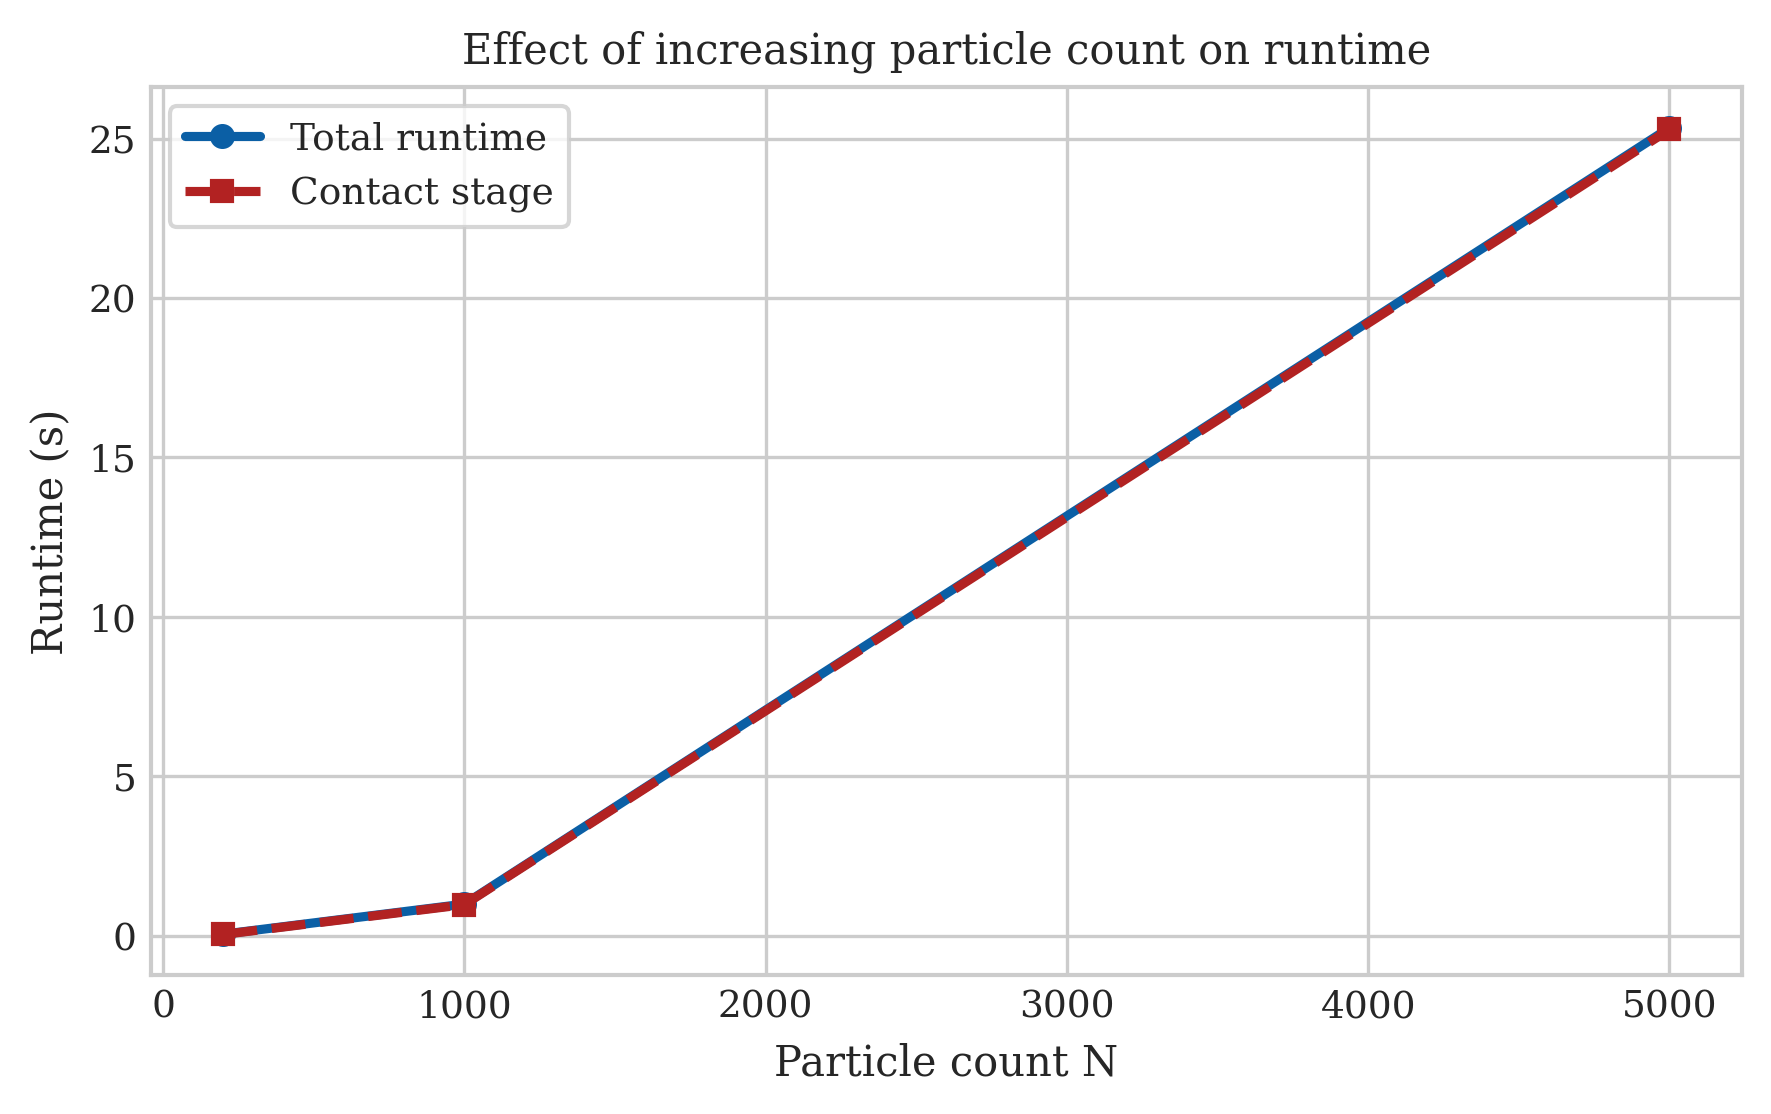
\includegraphics[width=\columnwidth]{figures/particle_count_runtime.png}
    \caption{Effect of increasing particle count on total runtime and contact-stage runtime.}
    \label{fig:particle_runtime}
\end{figure}

Figure~\ref{fig:particle_pairs} shows the corresponding growth in candidate pairs. The increase follows the expected all-pairs trend, which explains why contact detection becomes the dominant cost for larger systems. This plot is especially useful because it links the physical setup directly to computational cost: once the particle count increases, the solver is forced to examine many more potential interactions even before it decides whether contact actually occurs.

\begin{figure}[t]
    \centering
    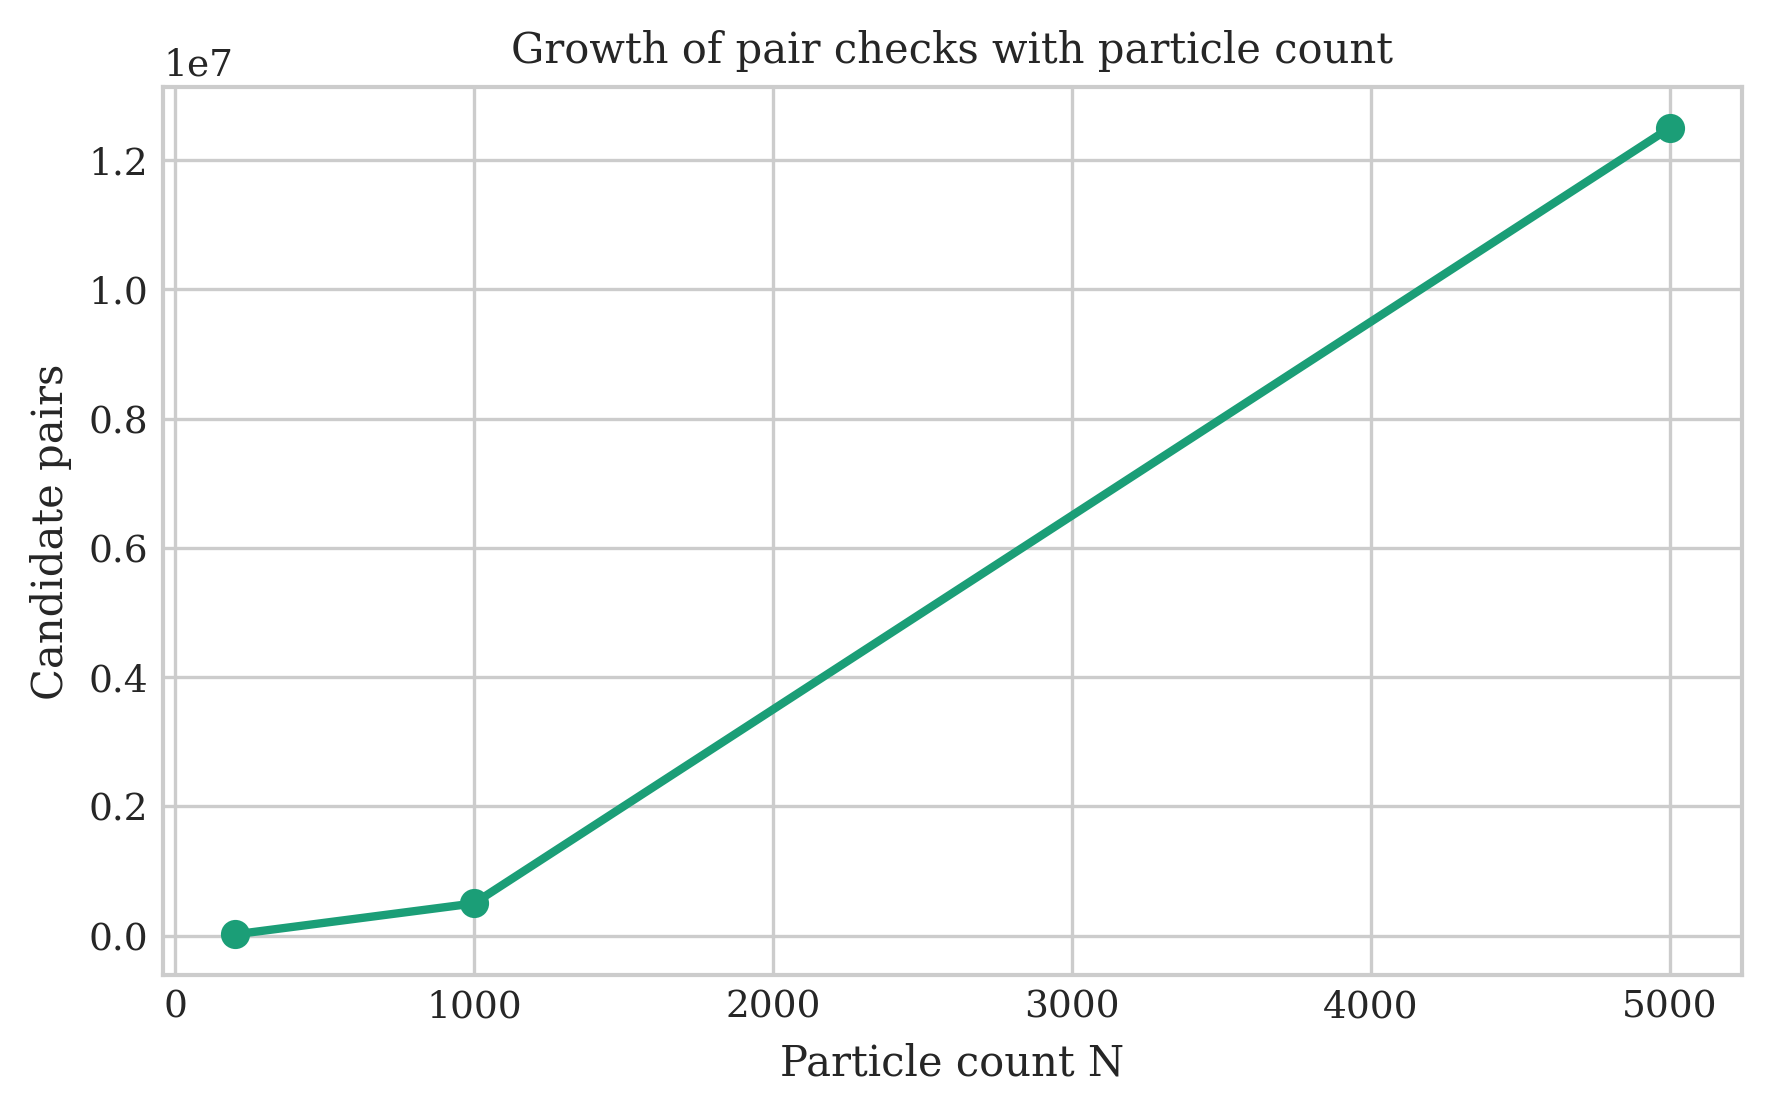
\includegraphics[width=\columnwidth]{figures/particle_count_candidate_pairs.png}
    \caption{Growth of candidate-pair checks with particle count in the brute-force serial solver.}
    \label{fig:particle_pairs}
\end{figure}

Figure~\ref{fig:particle_response} shows that increasing the particle count also changes the system-level response: the final kinetic energy and the maximum particle speed both increase for the larger cases. This is consistent with the fact that larger clouds create more interactions, more active collisions, and more opportunities for momentum exchange inside the box. So the multi-particle study is not only a runtime benchmark; it also shows that increasing $N$ changes the qualitative dynamical behaviour of the simulated system.

\begin{figure}[t]
    \centering
    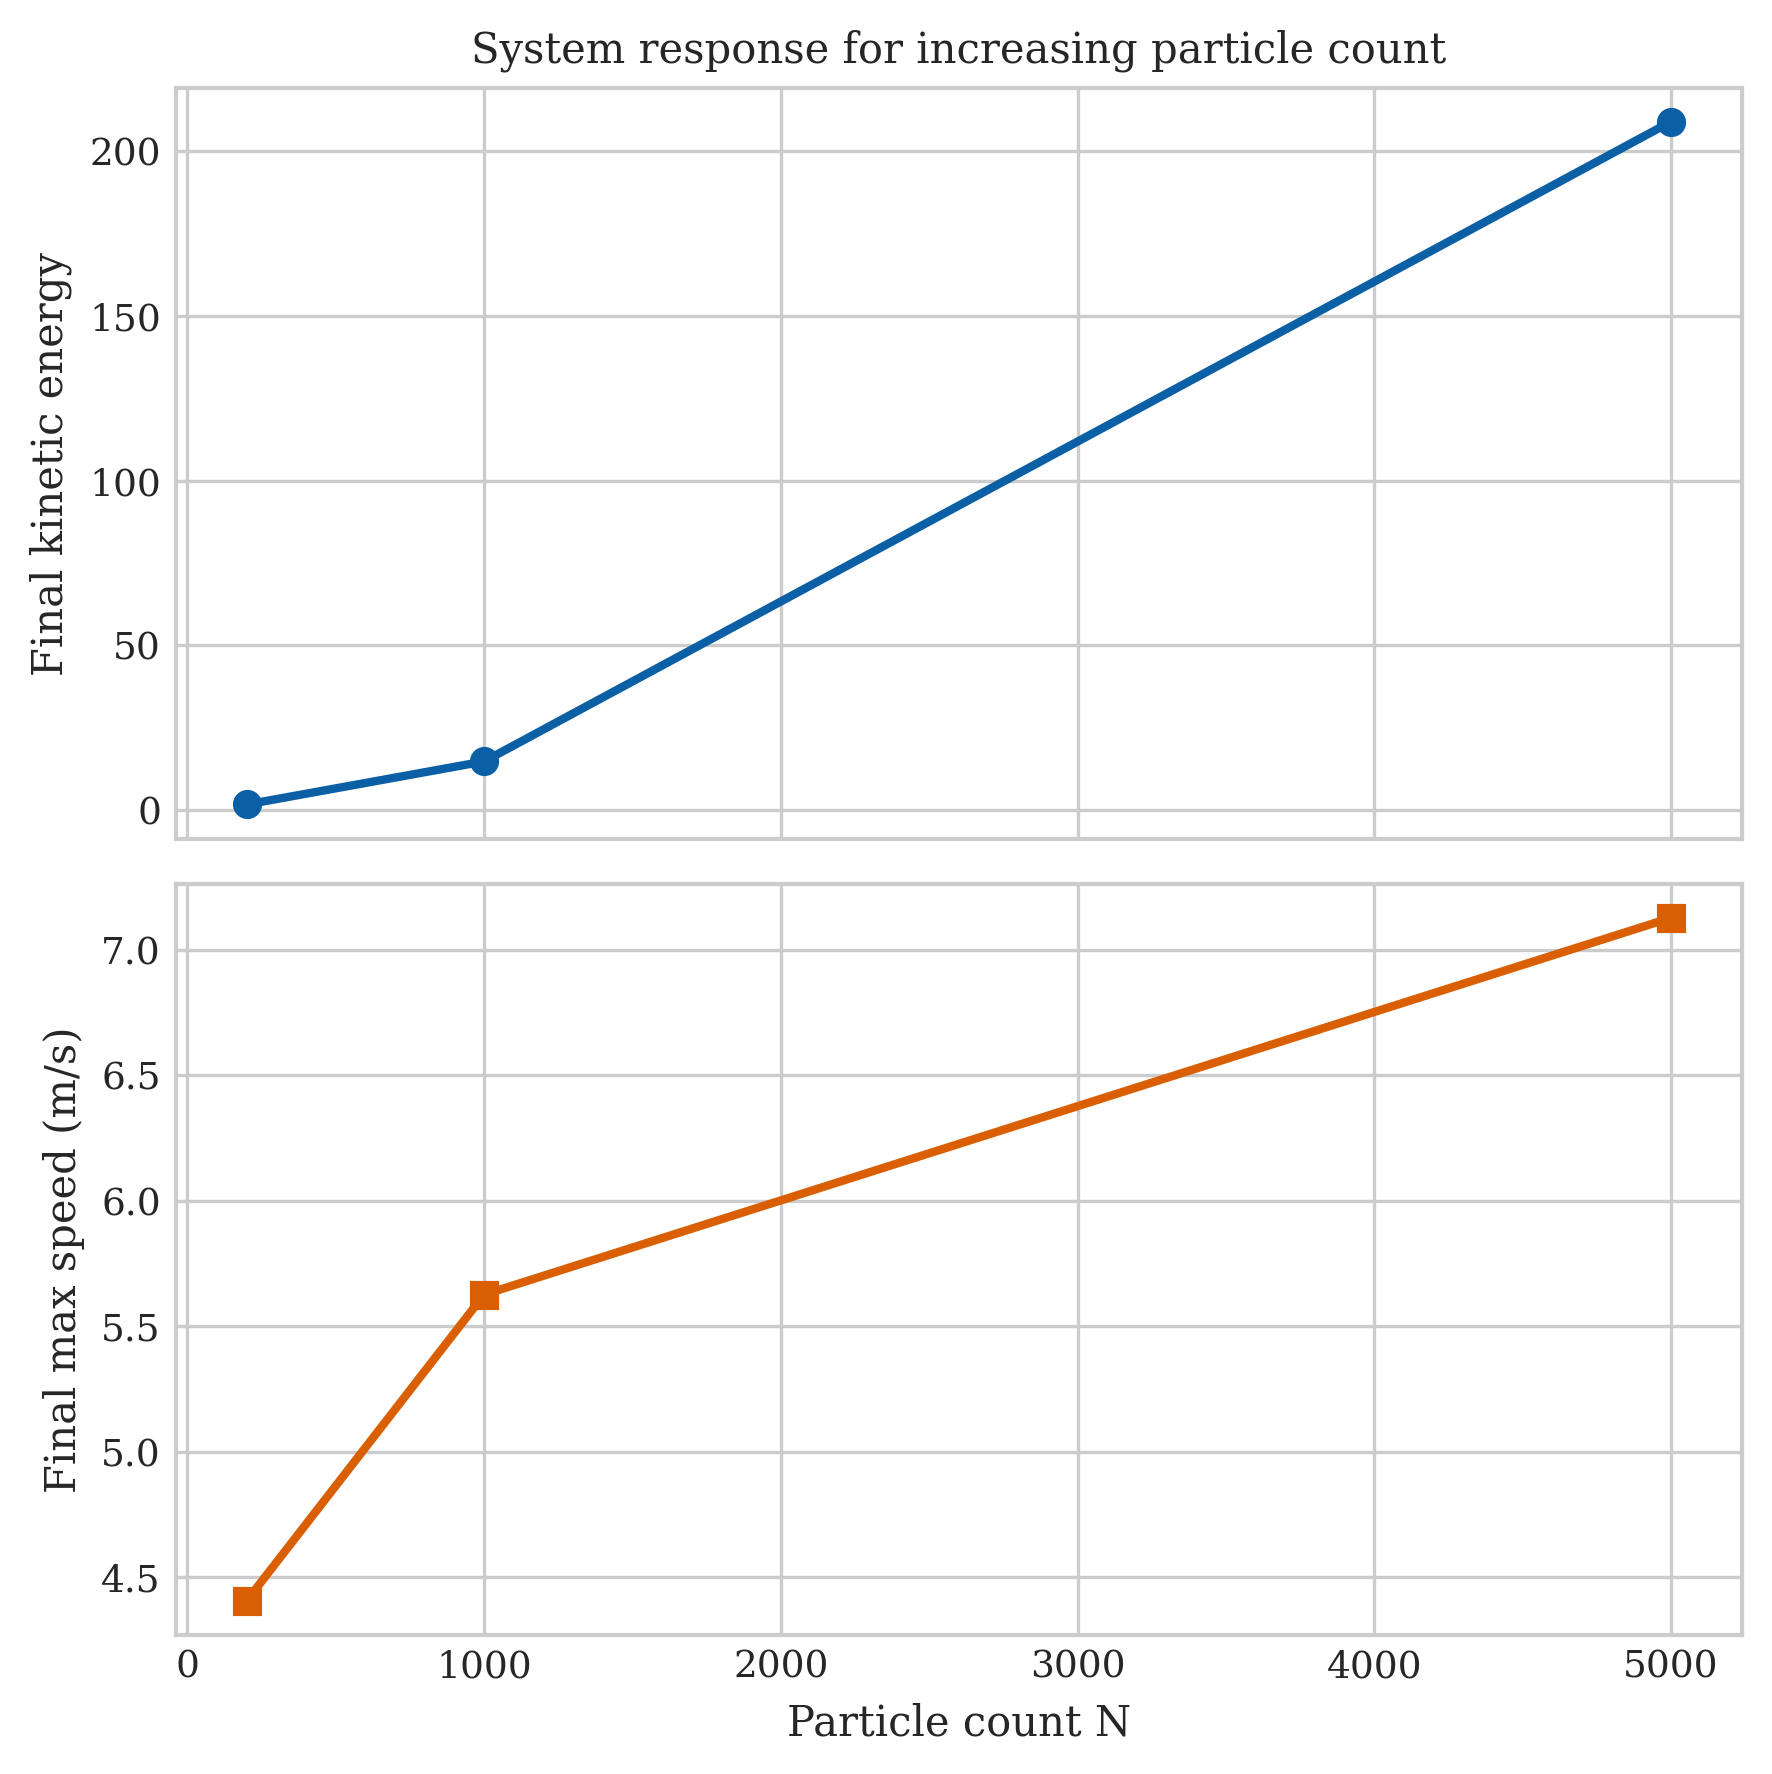
\includegraphics[width=\columnwidth]{figures/particle_count_system_response.png}
    \caption{System-response measures for increasing particle count.}
    \label{fig:particle_response}
\end{figure}

Taken together, these results show two important points. First, the assignment requirement to investigate increasing particle counts is satisfied explicitly for $N=200$, $1000$, and $5000$. Second, the results make it clear why profiling, OpenMP parallelisation, and neighbour search are needed: the cost of contact handling grows very quickly as the number of particles increases.

\section{Profiling Results}
The serial code was profiled by instrumenting the main stages of the timestep loop with \texttt{std::chrono::steady\_clock}. Rather than using an external profiling package, short scoped timers were placed around force reset, gravity, particle-contact evaluation, wall-contact handling, integration, and diagnostics. This made it possible to record both the total runtime of a full simulation and the runtime distribution across the major functions that appear in the solver.

The measured results show a very clear shift in cost as the number of particles increases. For the $N=200$ profiling run, the total runtime was about $0.0468$~s, with about $0.0381$~s already spent in particle-contact work alone. For the $N=1000$ case, the total runtime rose to about $0.9897$~s, of which about $0.9714$~s came from the particle-contact stage. By the time the system reaches $N=5000$, the full run takes about $25.3378$~s and about $25.2736$~s of that time is spent in particle-contact handling. In other words, once the particle count becomes moderate or large, almost the entire runtime is consumed by contact evaluation.

\begin{table}[t]
    \centering
    \scriptsize
    \caption{Runtime distribution across major functions for the serial profiling runs.}
    \label{tab:profiling}
    \setlength{\tabcolsep}{2pt}
    \resizebox{\columnwidth}{!}{%
    \begin{tabular}{rrrrrrr}
        \hline
        Particle count & Total (s) & Reset + gravity & Particle contacts & Wall contacts & Integration & Diagnostics \\
        \hline
        200 & 0.0468 & 0.0002 & 0.0381 & 0.0003 & 0.0003 & 0.0074 \\
        1000 & 0.9897 & 0.0013 & 0.9714 & 0.0019 & 0.0016 & 0.0130 \\
        5000 & 25.3378 & 0.0080 & 25.2736 & 0.0125 & 0.0109 & 0.0319 \\
        \hline
    \end{tabular}%
    }
\end{table}

Table~\ref{tab:profiling} makes the runtime distribution visible in a compact way. The gravity, integration, and diagnostics stages do contribute some cost, but their contribution stays small compared with the brute-force particle-particle contact loop. The candidate-pair counts reported for the same runs, namely $19{,}900$, $499{,}500$, and $12{,}497{,}500$, explain this behaviour directly: the serial all-pairs method grows quadratically with particle count, so contact detection becomes the computational bottleneck. This is why the contact stage was chosen for OpenMP parallelisation first, and later for neighbour-search optimisation.

Compiler optimisation was also enabled during the profiling study. All production builds used the \texttt{-O3} optimisation flag together with the normal warning flags. This means the reported runtimes are not from a debug-style build, but from an optimised executable that is closer to how the final solver should actually be run. Even with compiler optimisation enabled, the same bottleneck remained visible, which strengthens the conclusion that algorithmic and parallel improvements are needed in addition to compiler-level optimisation.

To quantify this point, the same serial experiment set was also compiled once with \texttt{-O0} and once with \texttt{-O3}. Figure~\ref{fig:compileropt} shows both the measured runtimes and the runtime ratio $T_{O0}/T_{O3}$, so the optimisation benefit is visible directly. For example, the $N=5000$ run dropped from about $233.93$~s at \texttt{-O0} to about $28.46$~s at \texttt{-O3}. This confirms that compiler optimisation is worthwhile, but it also shows that optimisation flags alone do not remove the all-pairs contact bottleneck.

\begin{figure}[t]
    \centering
    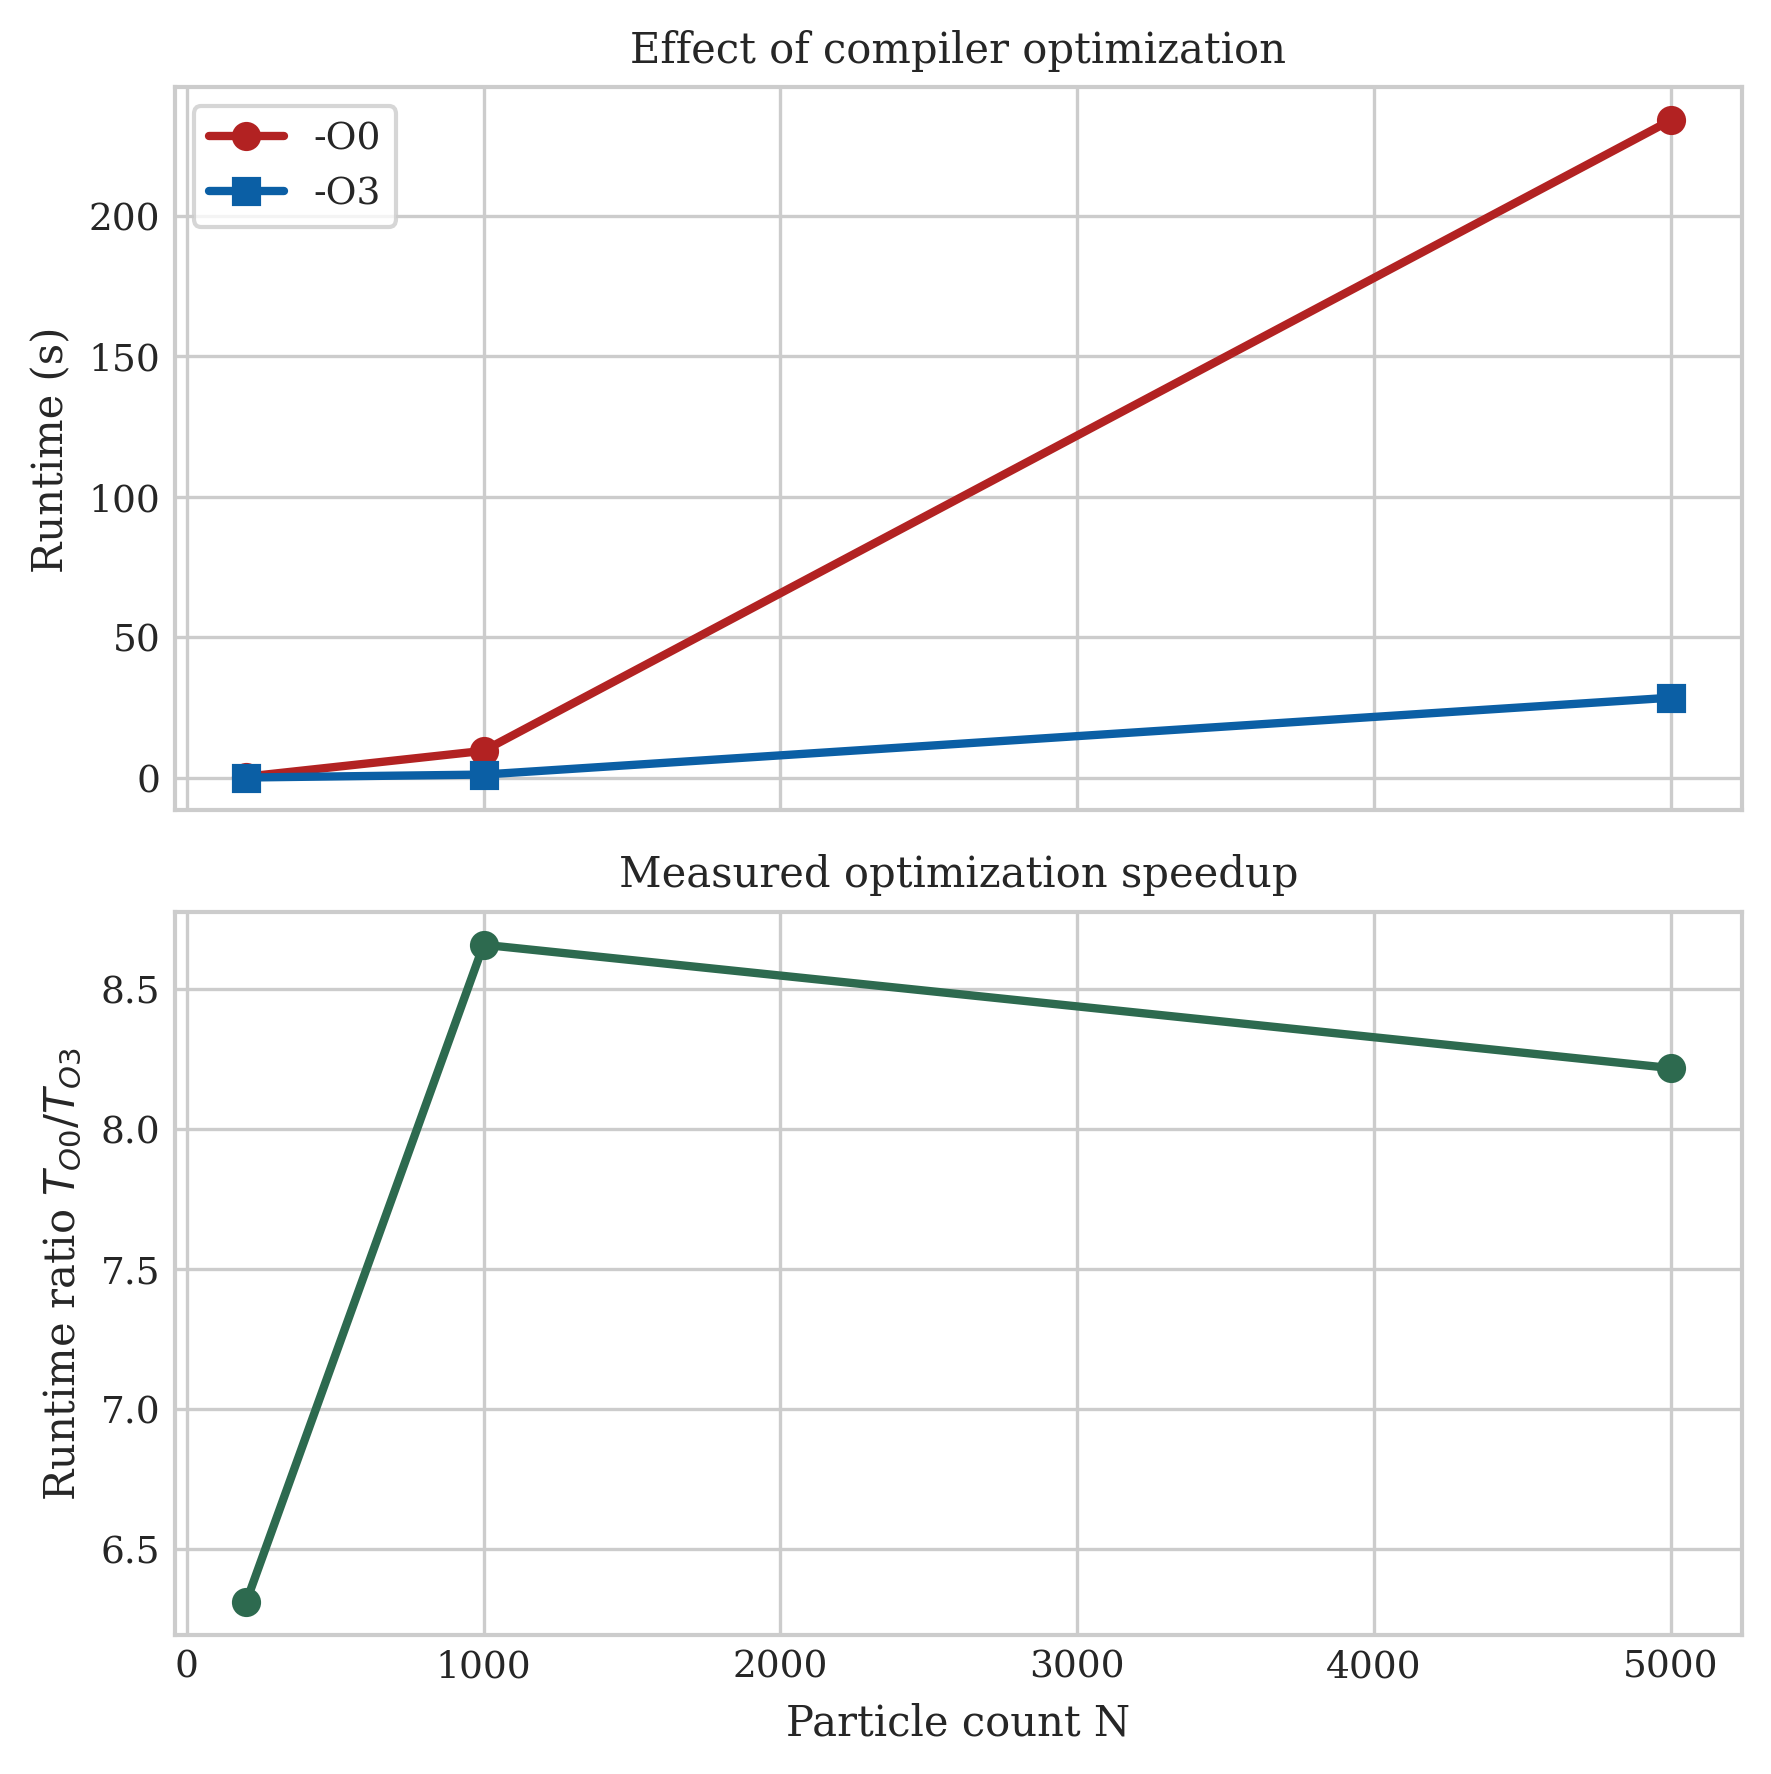
\includegraphics[width=\columnwidth]{figures/compiler_optimization_effect.png}
    \caption{Runtime comparison between unoptimised (\texttt{-O0}) and optimised (\texttt{-O3}) serial builds, together with the measured runtime ratio $T_{O0}/T_{O3}$.}
    \label{fig:compileropt}
\end{figure}

\section{Parallel Implementation}
OpenMP was applied to the particle-contact loop. A direct parallel update of shared particle forces would create race conditions, so thread-local force buffers were used instead. Each thread computes contact contributions for its assigned pair range and stores force increments locally. After the parallel region, the thread-local arrays are reduced into the global particle-force array.

This approach preserves numerical correctness while avoiding atomics on every contact-force update. The current implementation parallelises the brute-force all-pairs contact kernel because it is the dominant hotspot and because it has a simple work-sharing structure.

To verify that the parallel results match the serial results, the same physical case was run once with the serial contact loop and once with the OpenMP loop. The final diagnostic quantities were then compared directly. Table~\ref{tab:parallelcorrect} summarises the outcome for both $N=1000$ and $N=5000$. The final kinetic energy, maximum particle speed, center-of-mass height, and active-contact count are identical in the recorded output for both cases. This is strong evidence that parallelisation has not changed the numerical solution itself.

\begin{table}[t]
    \centering
    \scriptsize
    \caption{Serial-versus-parallel correctness check for matched physical cases.}
    \label{tab:parallelcorrect}
    \setlength{\tabcolsep}{3pt}
    \resizebox{\columnwidth}{!}{%
    \begin{tabular}{lcccc}
        \hline
        Quantity & $N$ & Serial & Parallel & Absolute diff. \\
        \hline
        Final kinetic energy & 1000 & 15.9320 & 15.9320 & 0 \\
        Max speed & 1000 & 5.4114 & 5.4114 & 0 \\
        Center-of-mass $z$ & 1000 & 0.7204 & 0.7204 & 0 \\
        Active contacts & 1000 & 5 & 5 & 0 \\
        Final kinetic energy & 5000 & 246.6795 & 246.6795 & 0 \\
        Max speed & 5000 & 7.1464 & 7.1464 & 0 \\
        Center-of-mass $z$ & 5000 & 0.7184 & 0.7184 & 0 \\
        Active contacts & 5000 & 391 & 391 & 0 \\
        \hline
    \end{tabular}%
    }
\end{table}

The same conclusion is illustrated visually in Figure~\ref{fig:parallelvel}, which compares serial and parallel velocity-component histories for a representative tracked particle for both $N=1000$ and $N=5000$. In every panel the OpenMP curve lies directly on top of the serial reference, so the velocity direction and magnitude are preserved after parallelisation. This is useful because it checks more than a single final scalar: it shows that the whole short-time motion history stays unchanged. Therefore, the parallelisation section does not only show that OpenMP was applied, but also that numerical correctness was preserved after the change.

\begin{figure}[t]
    \centering
    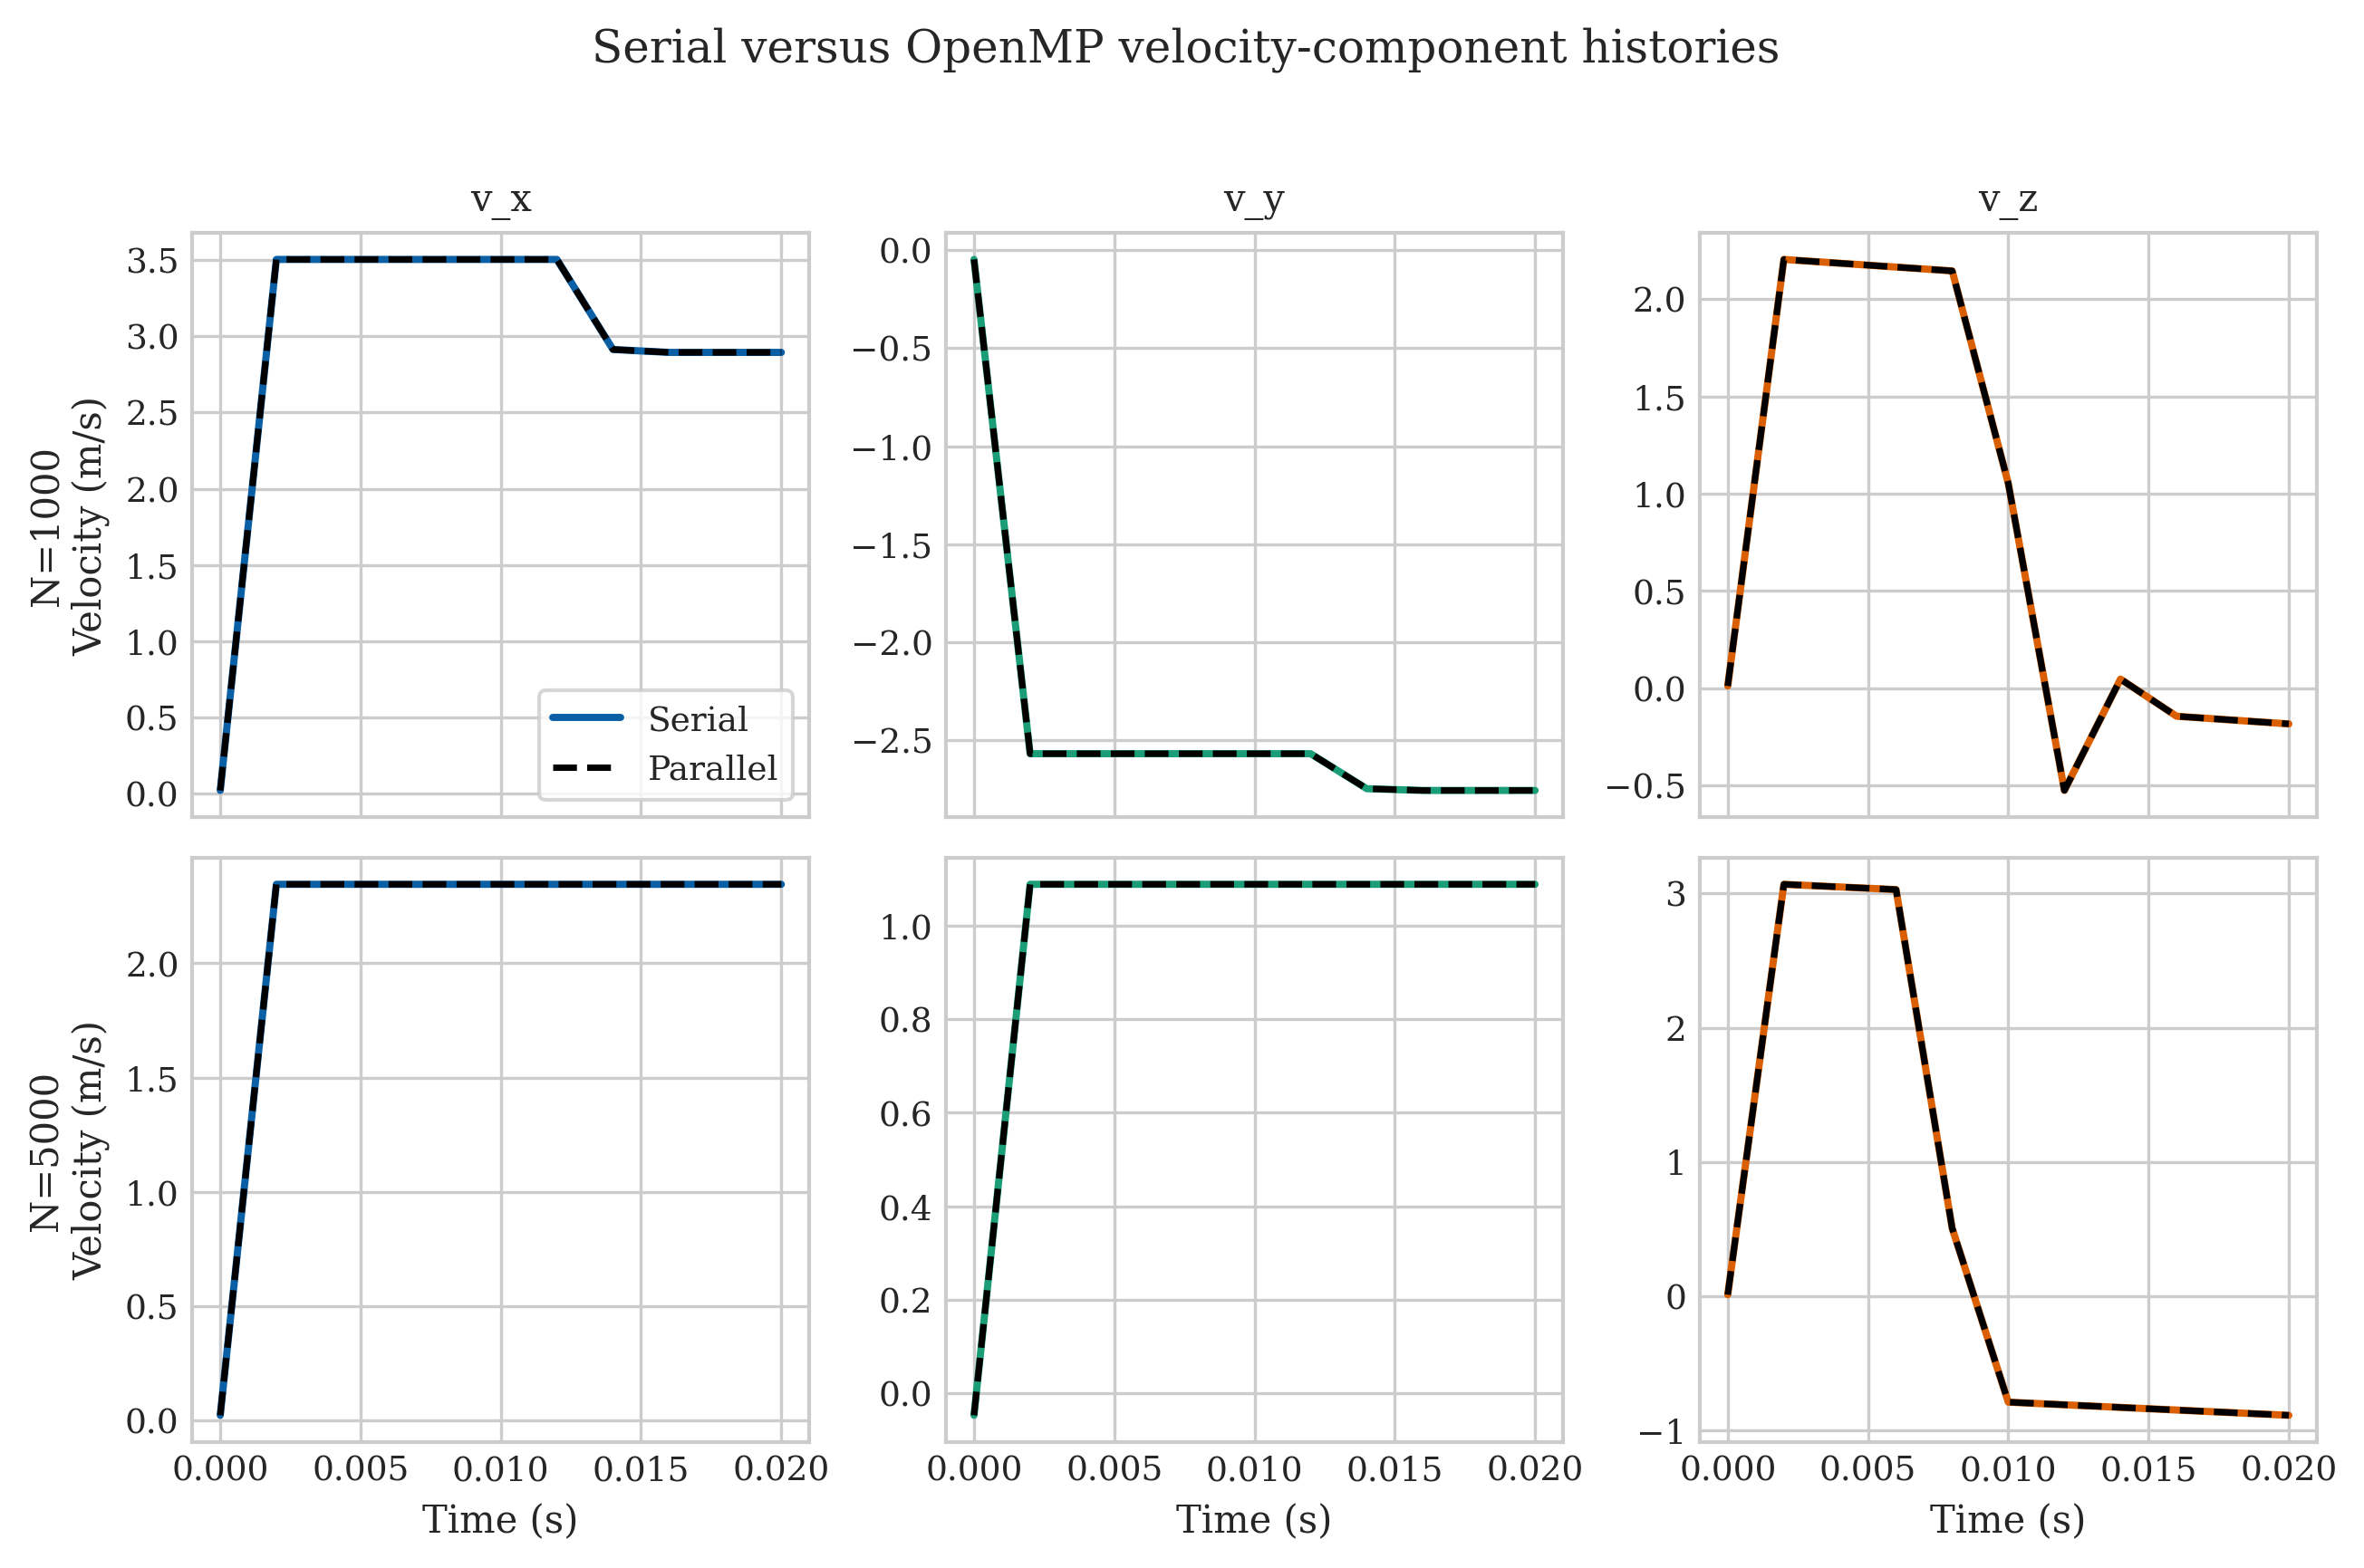
\includegraphics[width=\columnwidth]{figures/parallel_velocity_comparison.png}
    \caption{Serial-versus-parallel velocity-component histories for representative particles in the $N=1000$ and $N=5000$ correctness-check runs.}
    \label{fig:parallelvel}
\end{figure}

\section{Performance Analysis}
Two standard parallel-scaling viewpoints were considered. In strong scaling, the total problem size is kept fixed and only the thread count is increased. In weak scaling, the problem size is increased together with the thread count so that the work handled by each thread remains more nearly constant. These are the conventional definitions used in parallel-performance analysis, and the discussion below follows that standard terminology.

Before discussing the scaling plots, it is important to note that the profiling and scaling benchmarks are not identical. The profiling runs in Section~V use a simulated time of $0.03$~s, whereas the thread-scaling runs use a shorter simulated time of $0.02$~s. Therefore, the one-thread runtime for the $N=5000$ strong-scaling case is about $14.75$~s rather than the $35.08$~s seen in the profiling table. The purpose of the scaling benchmark is not to reproduce the profiling runtime exactly, but to compare thread counts fairly on the same fixed test case.

For the strong-scaling study, speedup and efficiency were computed for two fixed particle counts, $N=1000$ and $N=5000$. Table~\ref{tab:scaling} gives the measured runtimes, speedups, and efficiencies for thread counts from 1 to 8. Figure~\ref{fig:speedup} then visualises how the strong-scaling speedup changes with thread count, while Figure~\ref{fig:efficiency} shows how the parallel efficiency falls away from the ideal value as more threads are added.

\begin{table}[t]
    \centering
    \scriptsize
    \caption{Measured OpenMP strong-scaling results for $N=1000$ and $N=5000$.}
    \label{tab:scaling}
    \begin{tabular}{rcccccc}
        \hline
        Threads & $T_{1000}$ (s) & $S_{1000}$ & $E_{1000}$ & $T_{5000}$ (s) & $S_{5000}$ & $E_{5000}$ \\
        \hline
        1 & 0.5839 & 1.00 & 1.00 & 14.7498 & 1.00 & 1.00 \\
        2 & 0.5715 & 1.02 & 0.51 & 11.9067 & 1.24 & 0.62 \\
        4 & 0.3370 & 1.73 & 0.43 & 7.5919 & 1.94 & 0.49 \\
        8 & 0.3209 & 1.82 & 0.23 & 6.1116 & 2.41 & 0.30 \\
        \hline
    \end{tabular}
\end{table}

\begin{figure}[t]
    \centering
    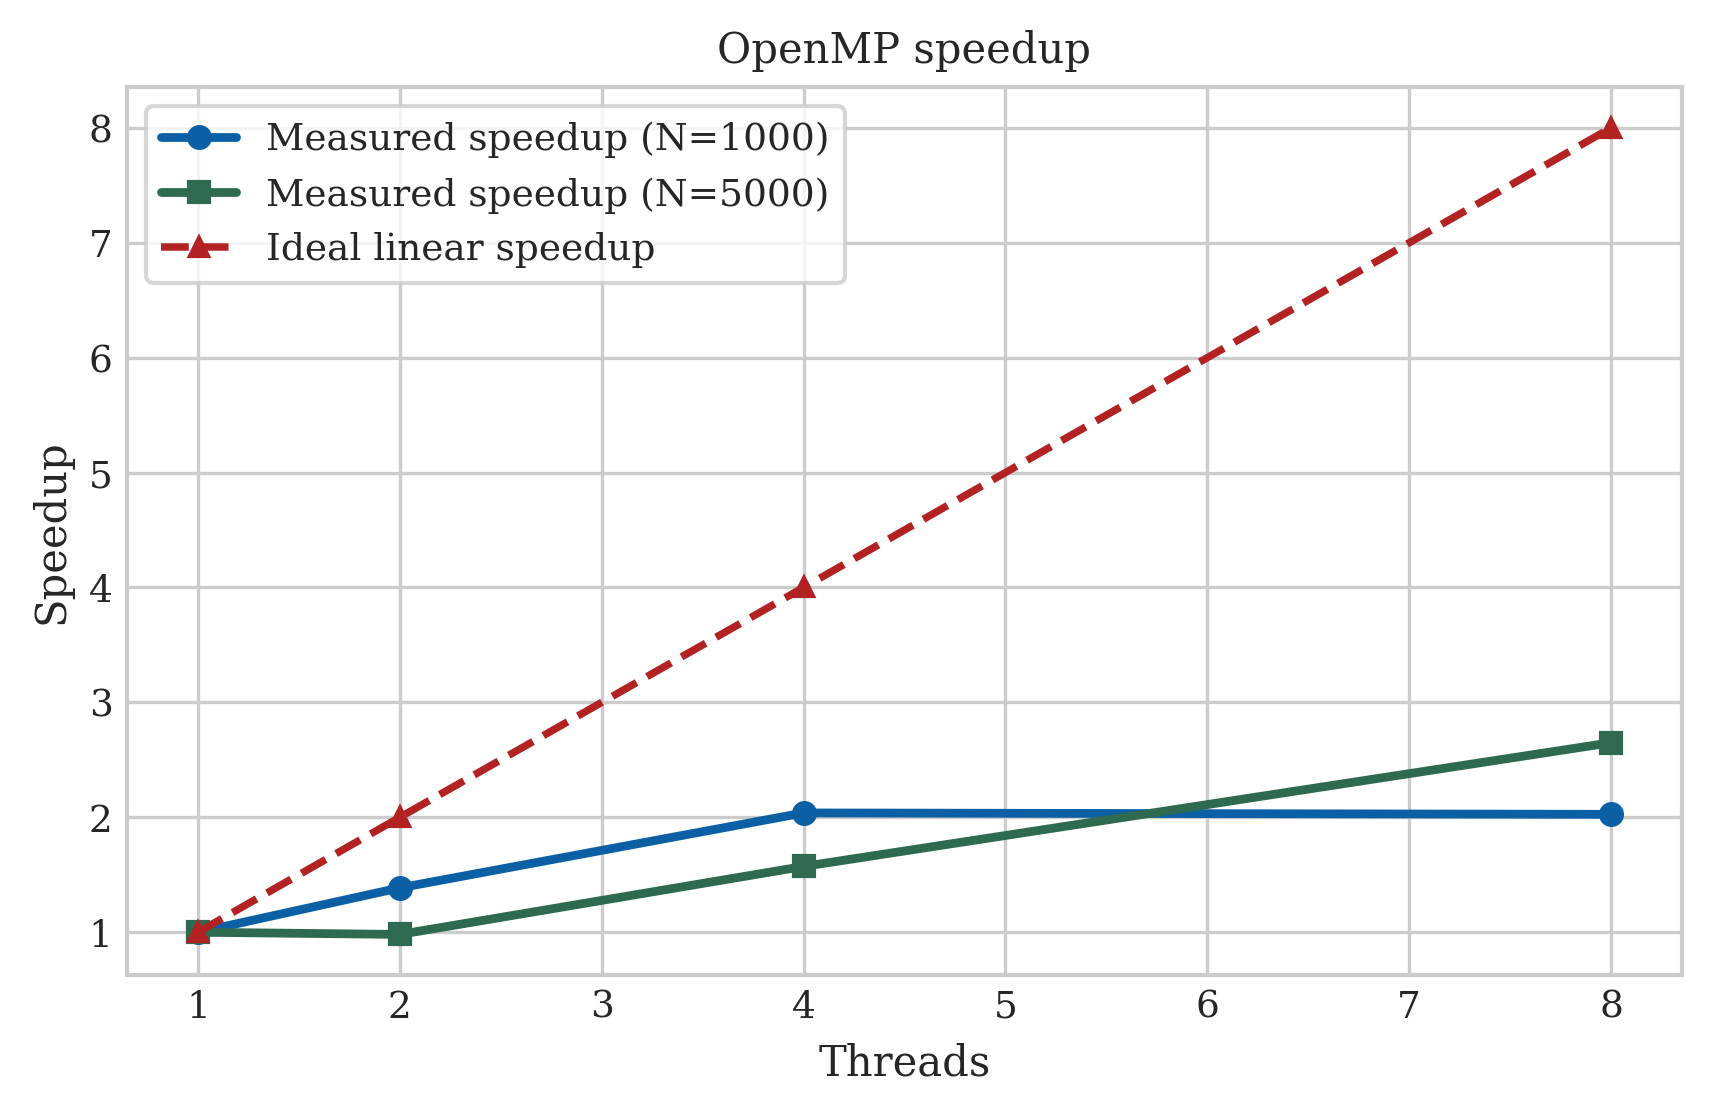
\includegraphics[width=\columnwidth]{figures/openmp_speedup.png}
    \caption{Measured OpenMP speedup compared with ideal linear scaling.}
    \label{fig:speedup}
\end{figure}

\begin{figure}[t]
    \centering
    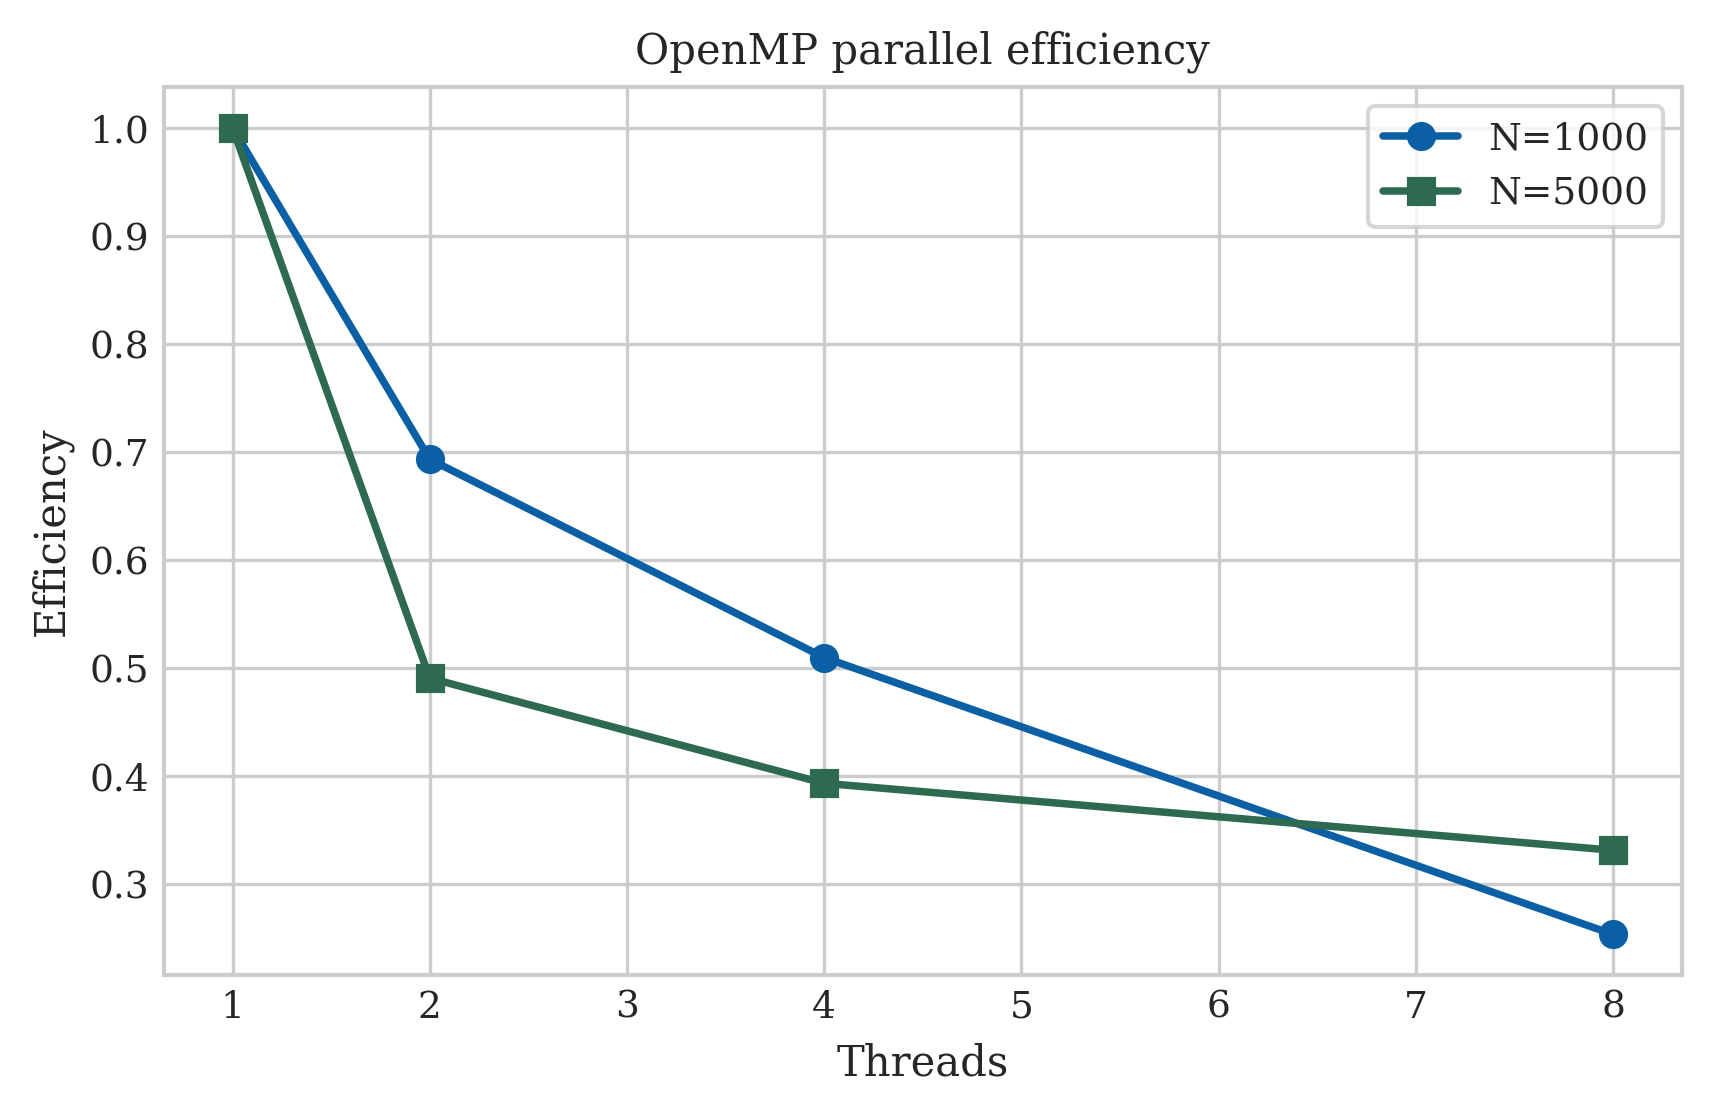
\includegraphics[width=\columnwidth]{figures/openmp_efficiency.png}
    \caption{Strong-scaling efficiency as a function of thread count.}
    \label{fig:efficiency}
\end{figure}

The measured strong-scaling speedup is sub-linear, which is expected. The main reasons are reduction overhead, memory traffic, and the remaining serial parts of the timestep loop. Even so, the trend is still useful: the parallel version becomes clearly faster than the one-thread version once the number of threads increases. The efficiency plot makes the same point from another angle: additional threads still help, but the per-thread benefit gradually decreases because the contact kernel is not the only cost inside a timestep.

The two strong-scaling curves also show that the larger $N=5000$ case benefits more consistently from extra threads than the $N=1000$ case. This is a typical shared-memory result. When the problem is relatively small, thread startup, buffer reduction, and other fixed overheads consume a larger fraction of the runtime, so the measured speedup stays modest. When the problem is larger, the parallel contact loop has more work to distribute, so those same overheads are amortised more effectively and the speedup improves. In that sense, the strong-scaling study answers the practical question: if the same DEM case is kept fixed, how much faster can it be solved by adding more OpenMP threads?

In summary, the strong-scaling results prove that the OpenMP implementation does accelerate fixed DEM problems, especially for the larger $N=5000$ case. The speedup is clearly better than 1 for higher thread counts, but it remains sub-linear because the code still contains serial work, memory traffic, and force-buffer reduction overhead. Therefore the parallel version is beneficial, but not ideally scalable.

\begin{figure}[t]
    \centering
    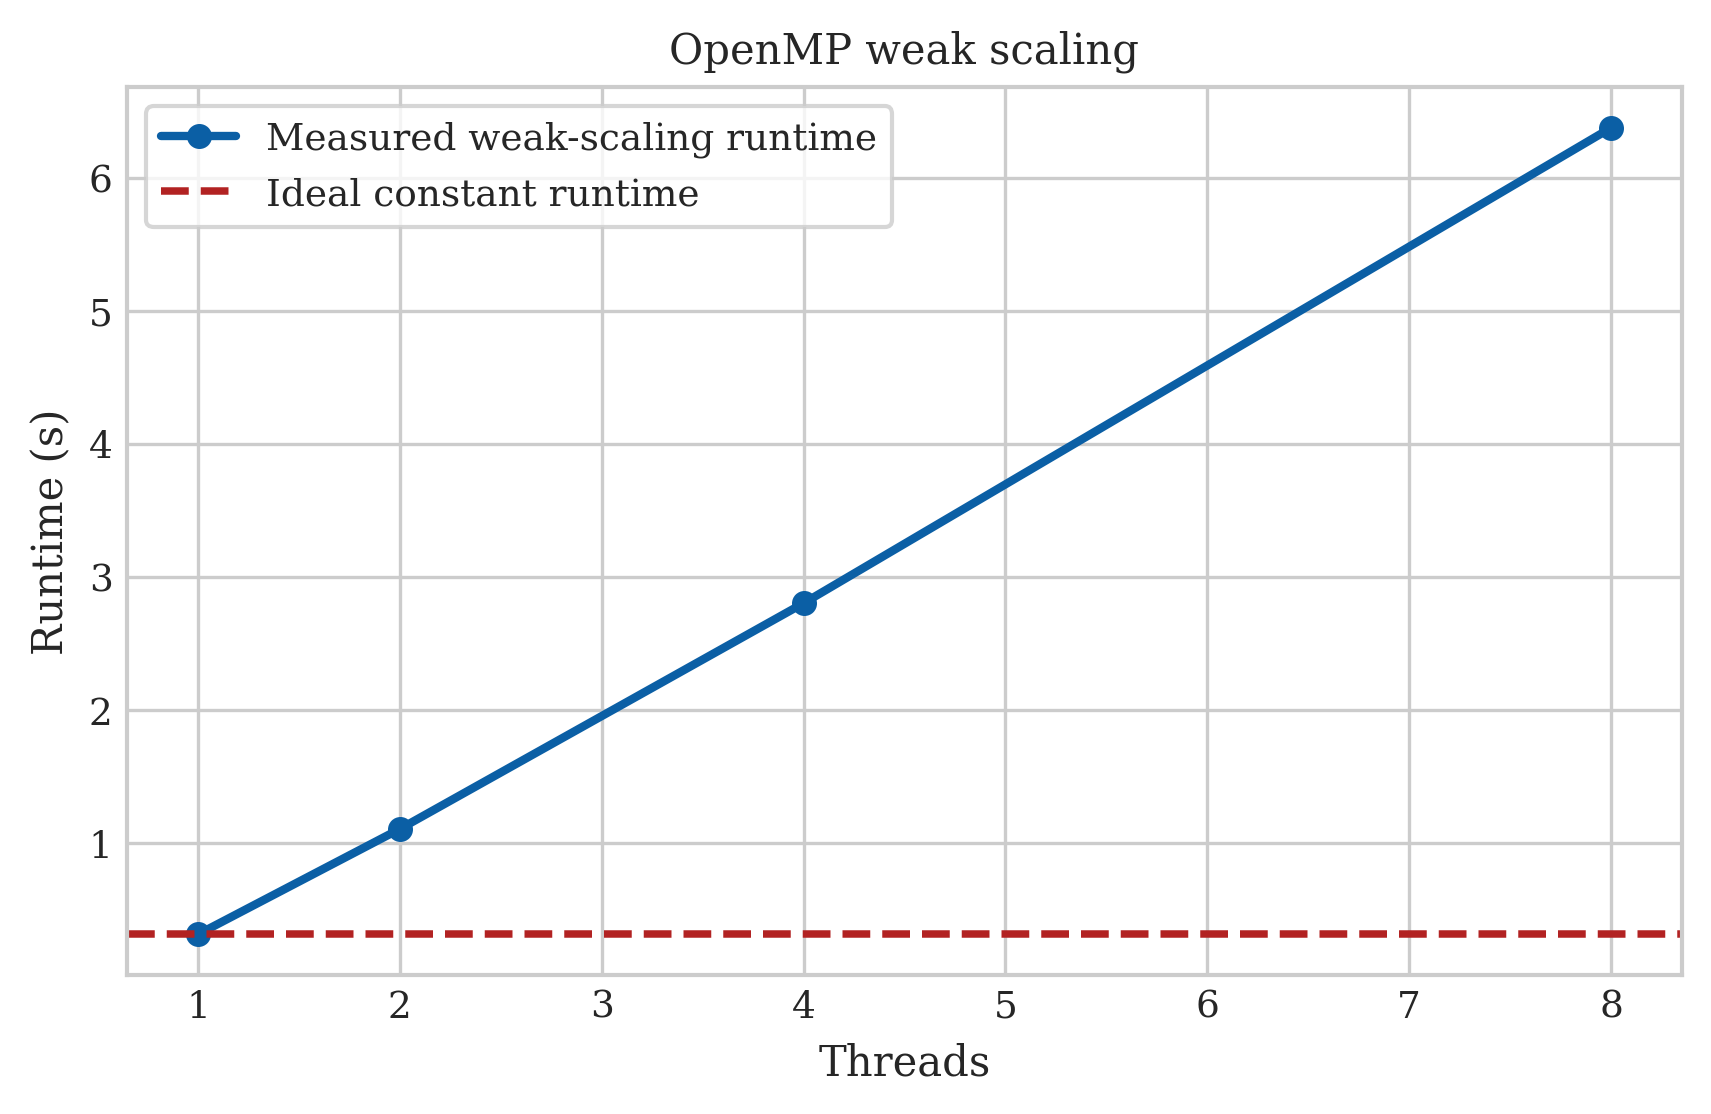
\includegraphics[width=\columnwidth]{figures/openmp_weak_scaling.png}
    \caption{Weak-scaling runtime as the problem size increases with thread count.}
    \label{fig:weakruntime}
\end{figure}

\begin{figure}[t]
    \centering
    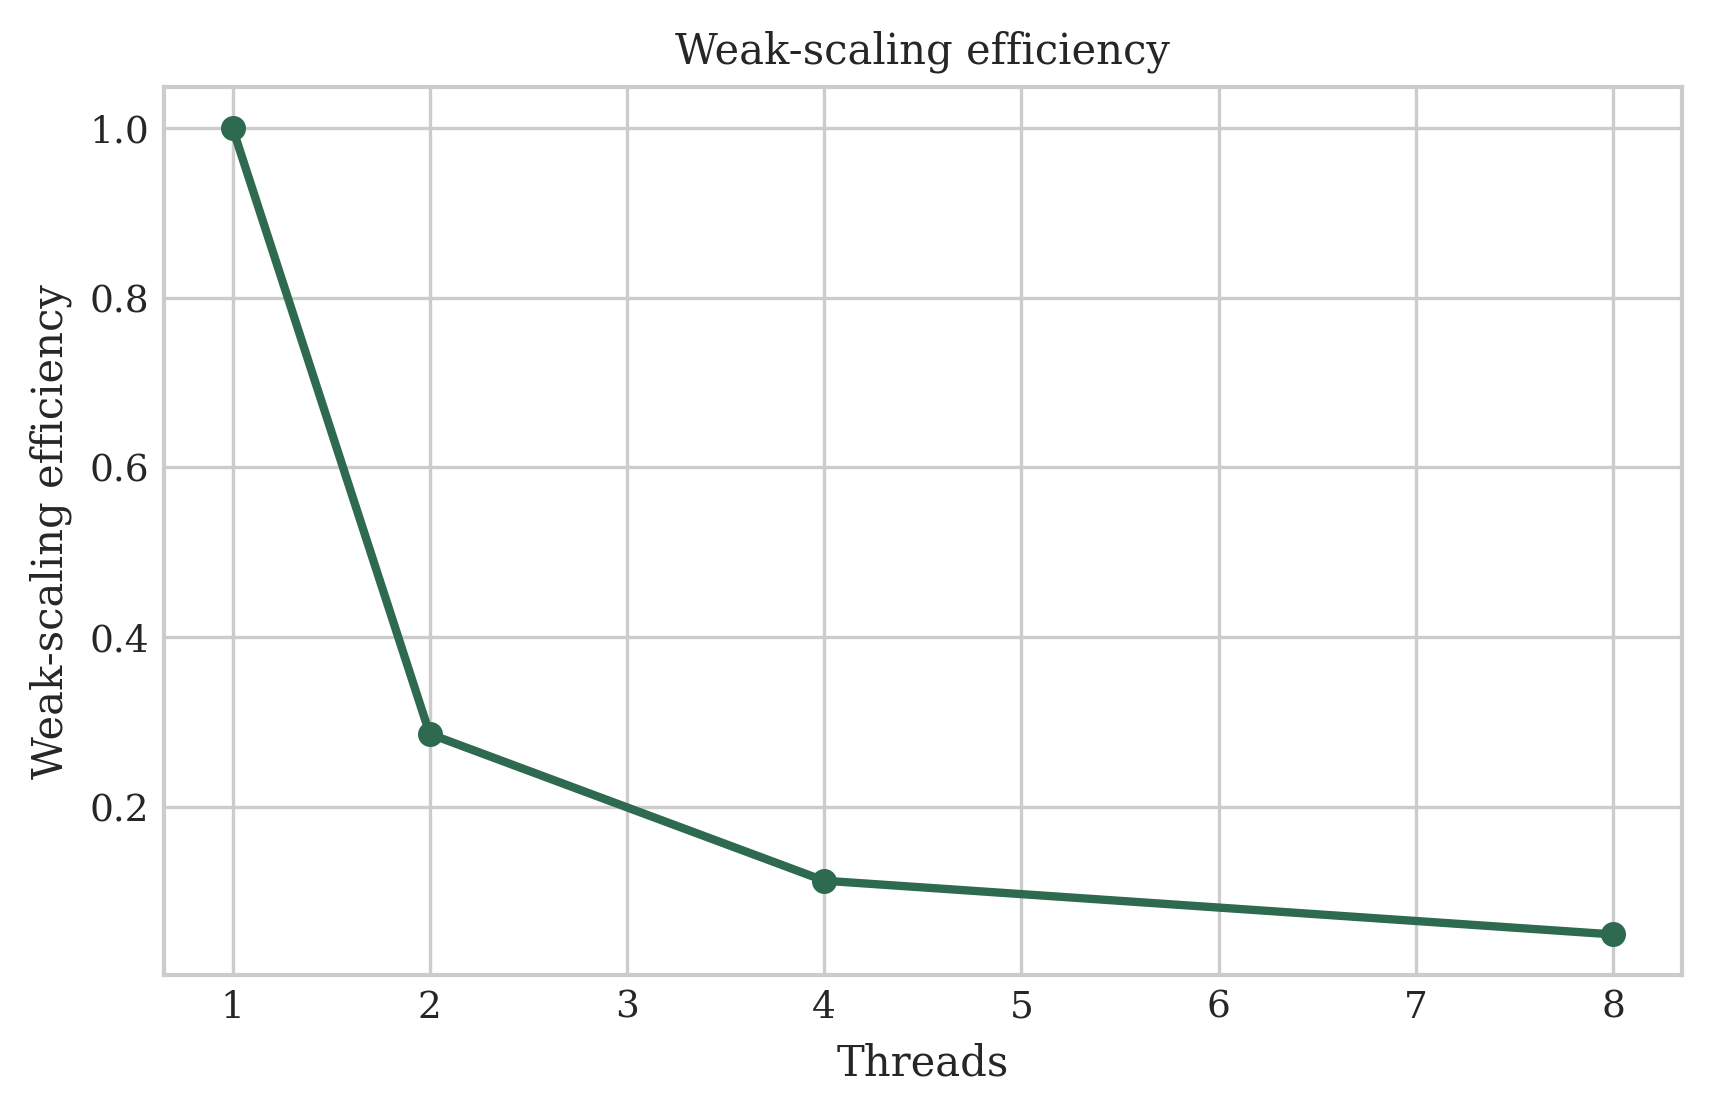
\includegraphics[width=\columnwidth]{figures/openmp_weak_efficiency.png}
    \caption{Weak-scaling efficiency for the OpenMP contact loop.}
    \label{fig:weakeff}
\end{figure}

\begin{table}[t]
    \centering
    \scriptsize
    \caption{Measured weak-scaling results with approximately constant particles per thread and density-preserving domain growth.}
    \label{tab:weakscaling}
    \begin{tabular}{rccccc}
        \hline
        Threads & Particles & Box length & Runtime (s) & Weak eff. & Overhead (s) \\
        \hline
        1 & 625 & 1.0000 & 0.3776 & 1.000 & 0.0000 \\
        2 & 1250 & 1.2599 & 1.0891 & 0.347 & 0.7115 \\
        4 & 2500 & 1.5874 & 2.8423 & 0.133 & 2.4647 \\
        8 & 5000 & 2.0000 & 6.4542 & 0.059 & 6.0766 \\
        \hline
    \end{tabular}
\end{table}

\begin{figure}[t]
    \centering
    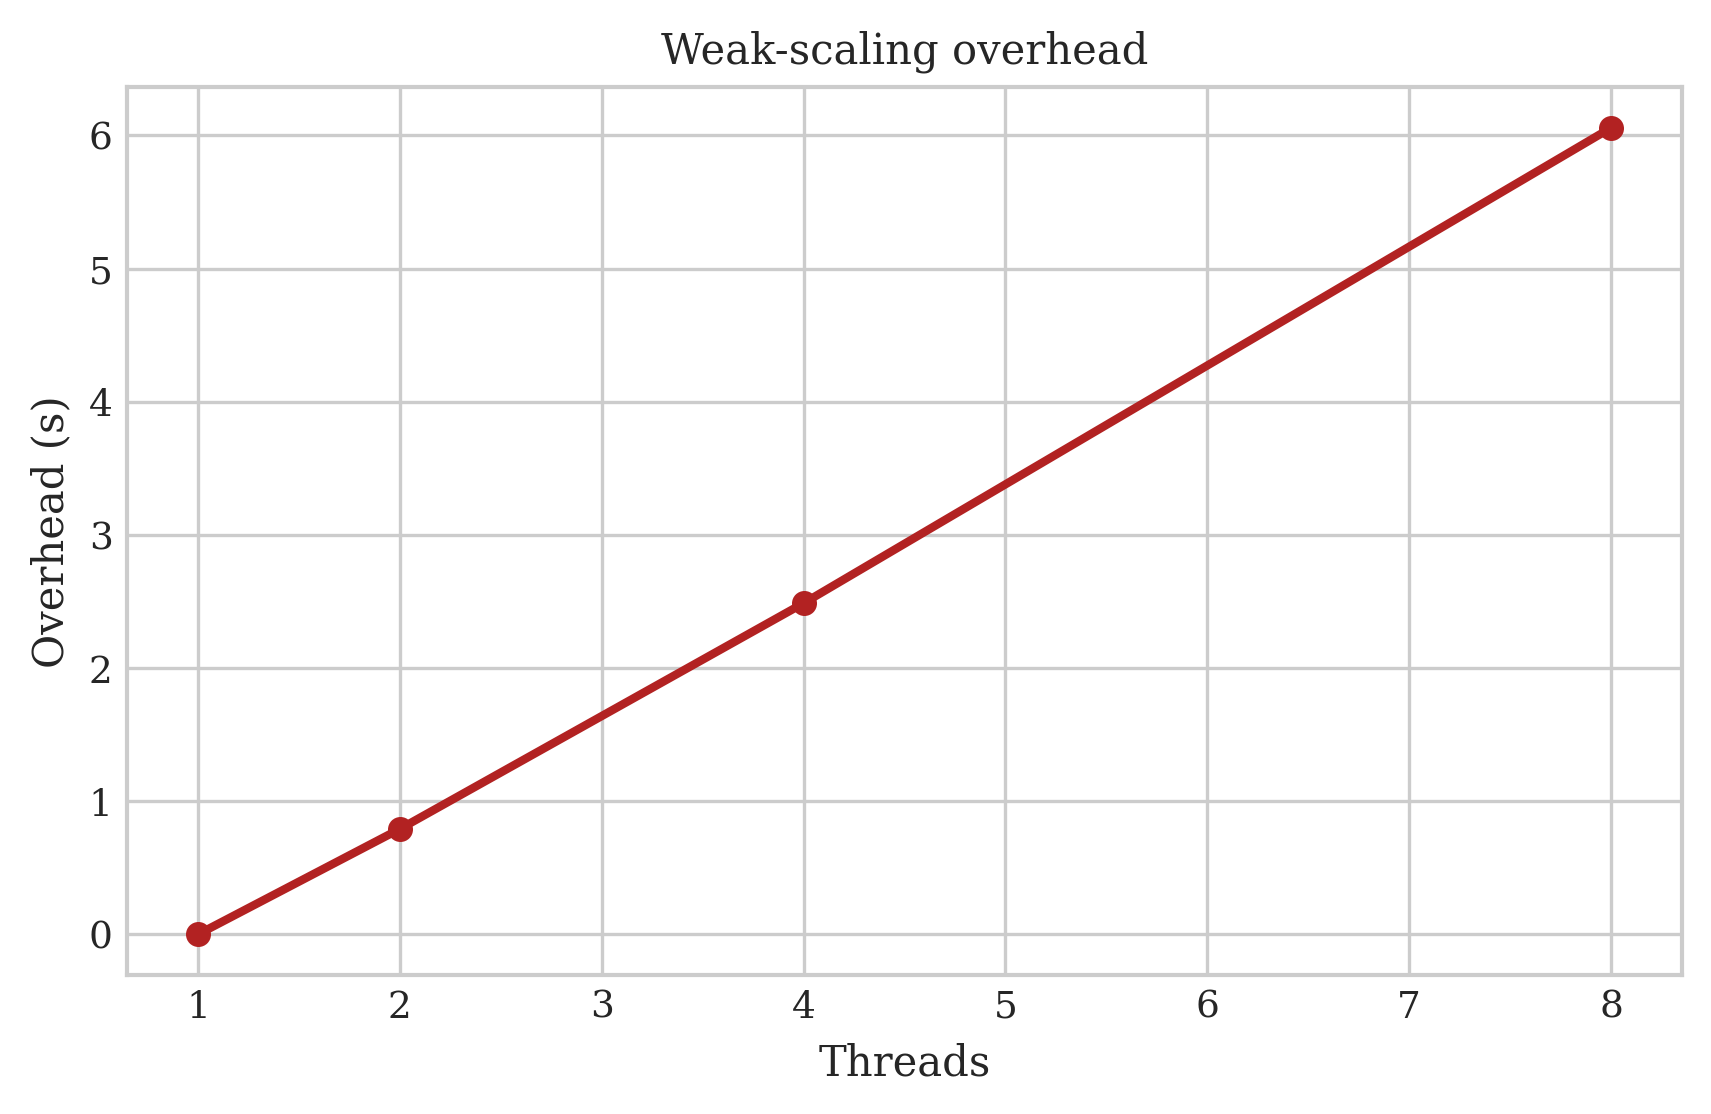
\includegraphics[width=\columnwidth]{figures/openmp_weak_overhead.png}
    \caption{Weak-scaling overhead relative to the one-thread baseline.}
    \label{fig:weakoverhead}
\end{figure}

The weak-scaling study was carried out in a DEM-specific way. The number of particles was increased with thread count, but the box size was also increased so that the particle density did not rise artificially. In practice the cubic box length was scaled as $L \propto p^{1/3}$, which keeps the domain volume proportional to the particle count. This is important for DEM because changing the particle count without changing the box size would change the packing density and therefore the underlying physics.

The measured weak-scaling results in Table~\ref{tab:weakscaling} and Figures~\ref{fig:weakruntime}--\ref{fig:weakoverhead} show that the implementation does not scale weakly in an ideal sense. If it did, the runtime would remain almost constant as both particle count and thread count increased. Instead, the runtime rises from about $0.38$~s at $(1,625)$ to about $6.45$~s at $(8,5000)$, the weak-scaling efficiency drops well below 1, and the overhead grows steadily with thread count.

Even so, the weak-scaling study is still useful because it shows how quickly the shared-memory costs accumulate when larger DEM systems are attempted. The increase in runtime reflects several effects acting together: a larger all-pairs candidate set, more memory traffic, and the extra work of reducing thread-local force buffers back into the shared particle array. Therefore the present OpenMP implementation extends the solvable problem size, but it does not preserve constant runtime as the total problem size grows.

In summary, the weak-scaling study proves that the current OpenMP solver can handle larger DEM systems when more threads are provided, but it does not maintain near-constant runtime under density-preserving problem growth. The rising runtime, falling weak efficiency, and increasing overhead all show that weak scaling is limited by the brute-force contact strategy and shared-memory overheads.

\section{Bonus Extension: Neighbour Search}
To reduce the cost of contact detection, a uniform cell-linked neighbour grid was implemented. The box is divided into cubic cells whose width is chosen from the particle size, so any possible overlap must occur either inside one cell or across one of its neighbouring cells. At each timestep, every particle is reassigned to a cell based on its current position. The contact loop then visits each occupied cell and checks particle pairs only within that cell and the 26 neighbouring cells, while still applying exactly the same spring-dashpot force model as in the brute-force solver. Therefore, the neighbour-search implementation changes only the search strategy, not the underlying DEM physics.

In practical terms, the implementation has three stages inside each timestep: grid rebuild, local candidate-pair traversal, and the same contact-force evaluation already used in the serial all-pairs code. This makes the method easy to compare fairly against the brute-force baseline, because the only algorithmic change is the reduction in the number of candidate pairs presented to the contact model.

The neighbour-search algorithm used in each timestep can therefore be summarised as follows:
\begin{enumerate}
\item divide the simulation box into uniform cubic cells,
\item assign each particle to a cell from its current position,
\item for each occupied cell, visit the same cell and the 26 neighbouring cells,
\item generate candidate particle pairs only from those local cell combinations,
\item evaluate the usual DEM contact force only for those candidate pairs,
\item accumulate the resulting forces and continue with wall contacts and time integration.
\end{enumerate}

This algorithm is equivalent to the brute-force method in the sense that the same contact model is still applied, but it avoids testing pairs that are too far apart to overlap.

\begin{table}[t]
    \centering
    \scriptsize
    \caption{Brute-force versus neighbour-grid comparison for three particle counts.}
    \label{tab:neighbor}
    \setlength{\tabcolsep}{3pt}
    \resizebox{\columnwidth}{!}{%
    \begin{tabular}{r l r r r r}
        \hline
        $N$ & Method & Total runtime (s) & Contact stage (s) & Candidate pairs & Active contacts \\
        \hline
        200 & All pairs & 0.0151 & 0.0119 & 19,900 & 0 \\
        200 & Grid & 0.0195 & 0.0111 & 19 & 0 \\
        1000 & All pairs & 0.3477 & 0.3408 & 499,500 & 2 \\
        1000 & Grid & 0.0464 & 0.0303 & 400 & 2 \\
        5000 & All pairs & 8.9849 & 8.9646 & 12,497,500 & 96 \\
        5000 & Grid & 0.1339 & 0.1033 & 10,298 & 96 \\
        \hline
    \end{tabular}%
    }
\end{table}

Table~\ref{tab:neighbor} gives the full comparison requested in the assignment: correctness of detected contacts, total runtime, contact-stage runtime, candidate-pair count, and scaling with particle number. The correctness result is especially clear because the active-contact counts match exactly for all three test sizes. For $N=200$, both methods detect zero active contacts; for $N=1000$, both detect 2 contacts; and for $N=5000$, both detect 96 contacts. This supports the conclusion that the neighbour grid changes the search cost, not the detected-contact outcome for these test cases.

\begin{figure}[t]
    \centering
    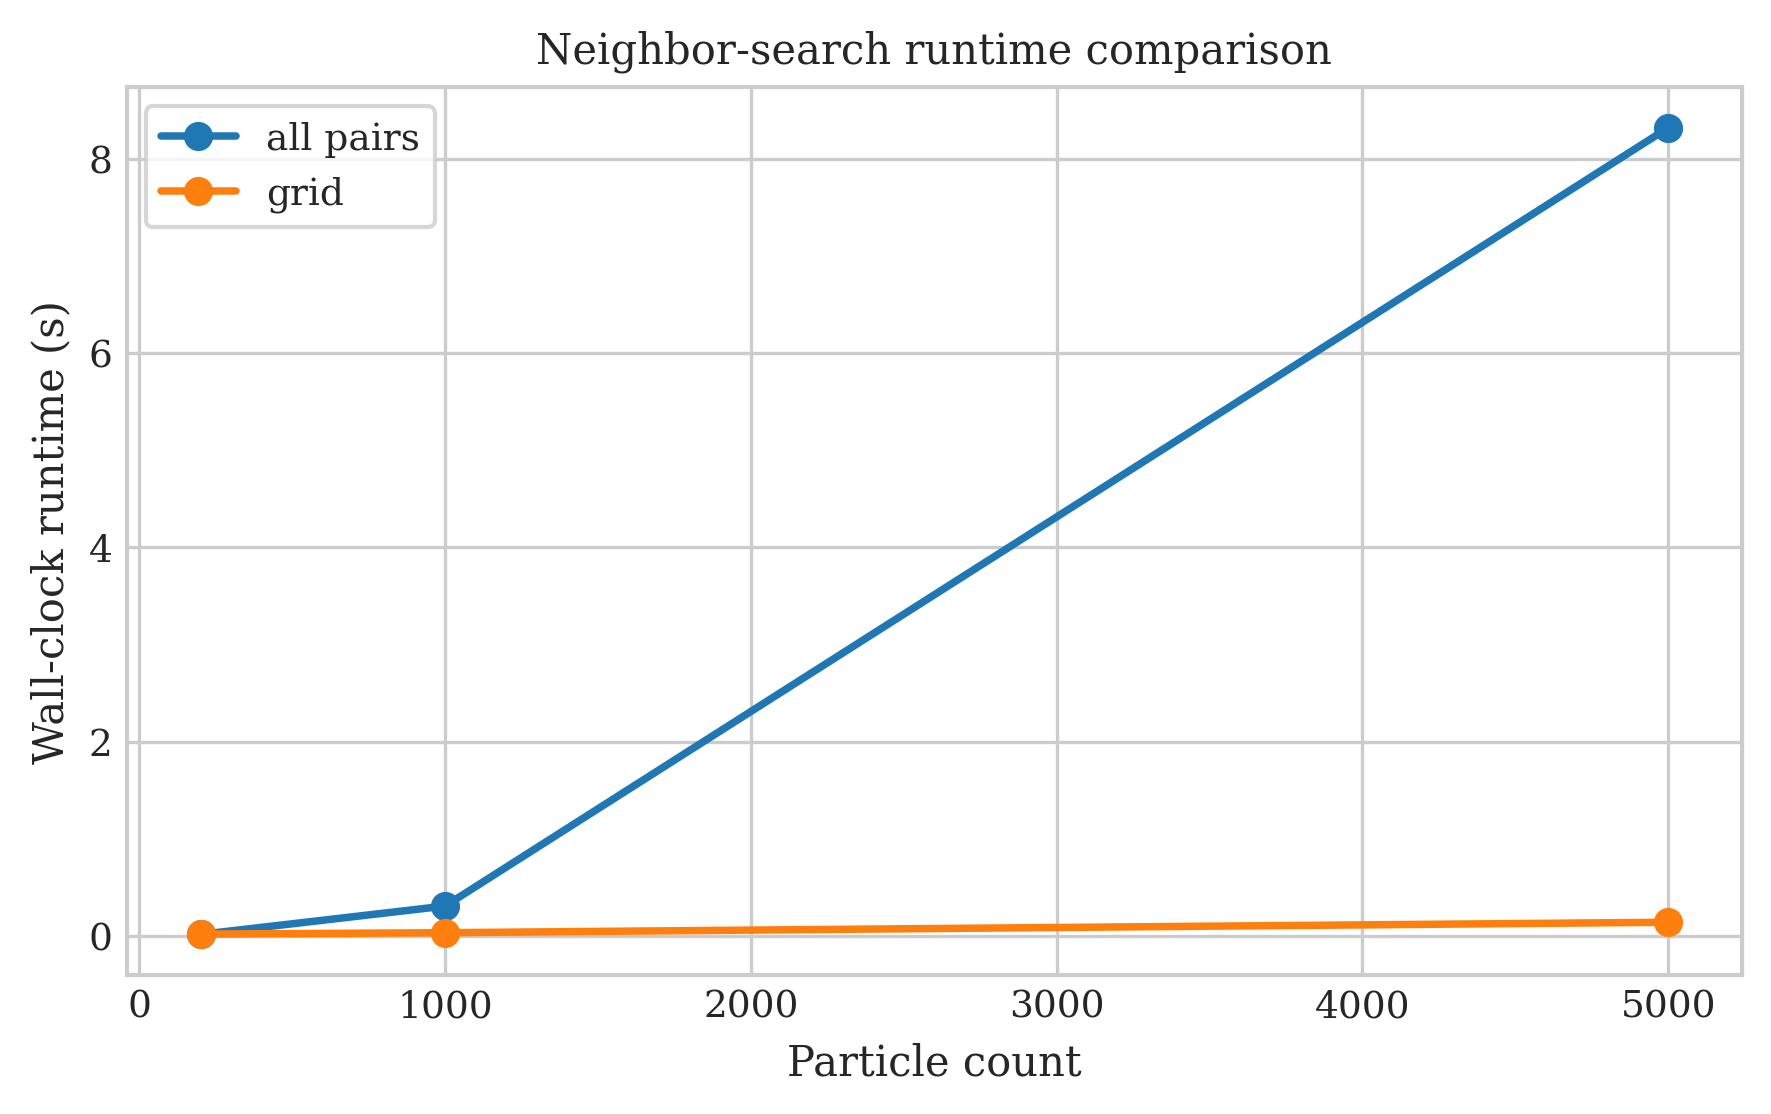
\includegraphics[width=\columnwidth]{figures/neighbor_runtime_comparison.png}
    \caption{Total runtime comparison of brute-force all-pairs search and neighbour-grid search for three particle counts.}
    \label{fig:neighbor_runtime}
\end{figure}

\begin{figure}[t]
    \centering
    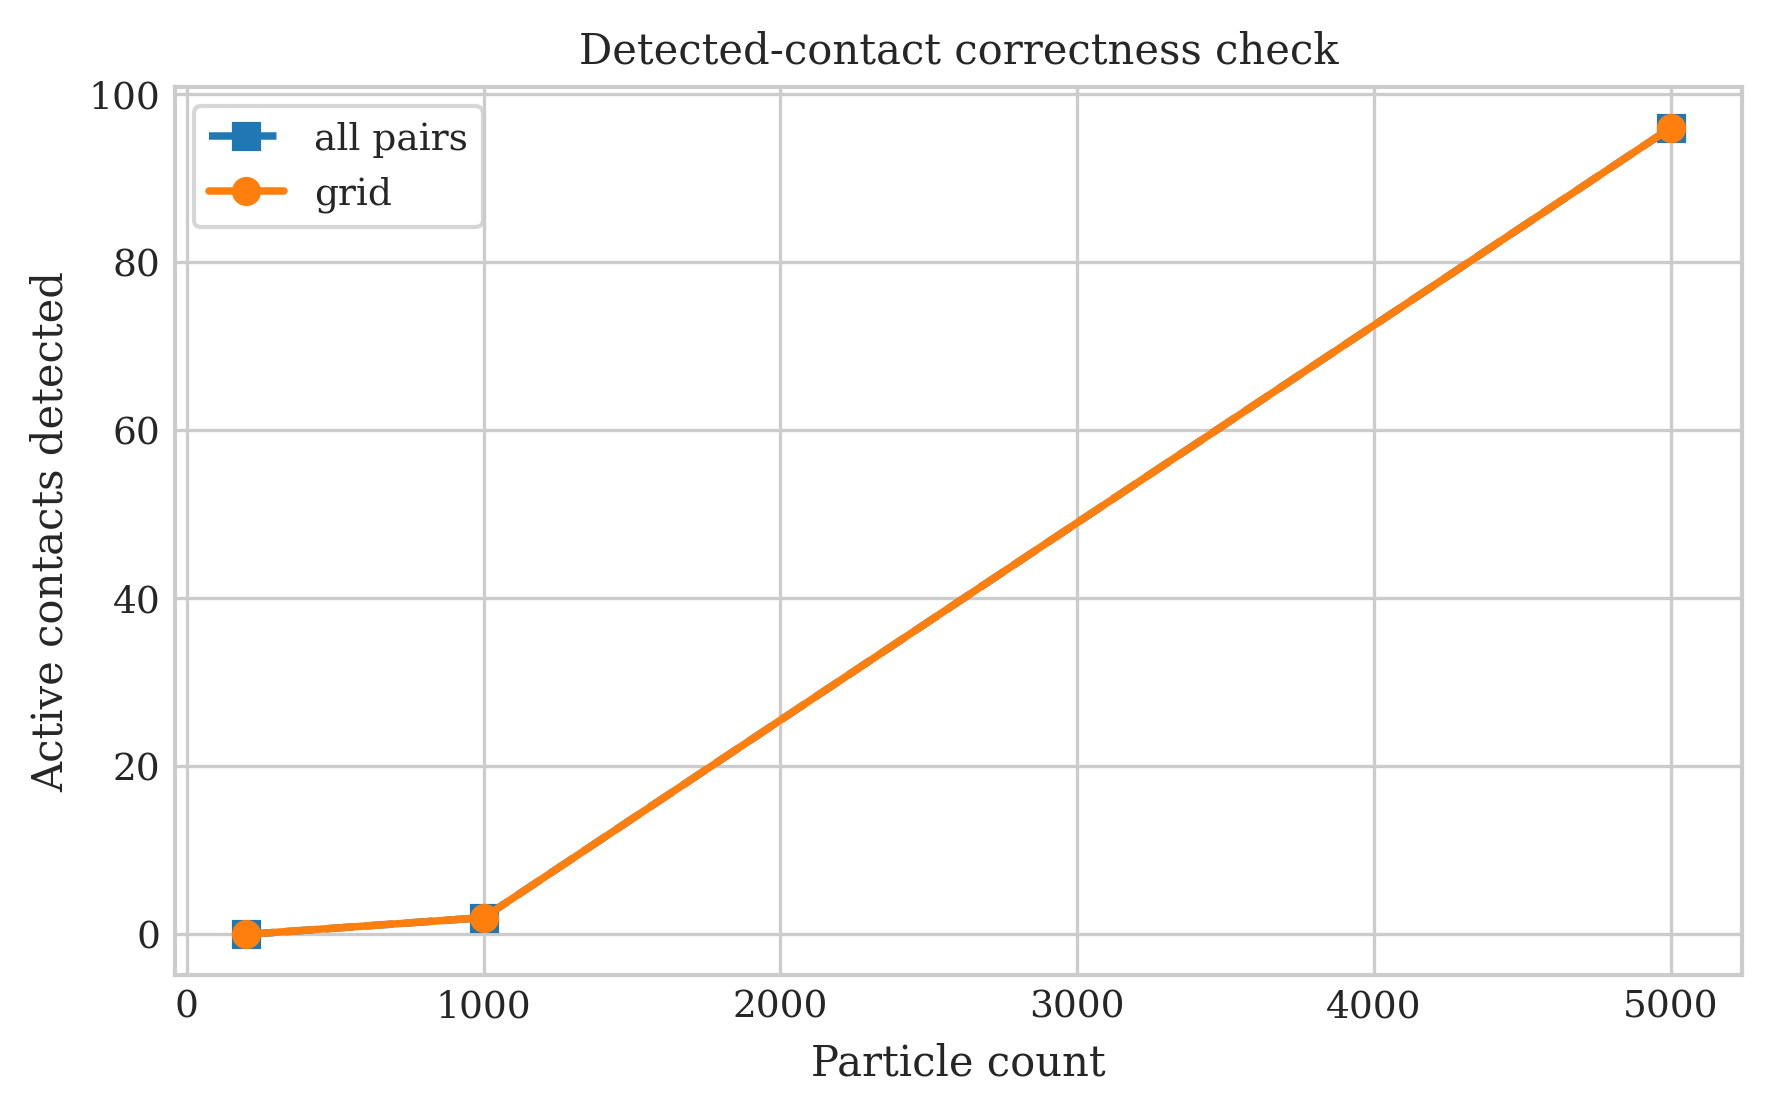
\includegraphics[width=\columnwidth]{figures/neighbor_active_contacts.png}
    \caption{Detected active-contact counts for the brute-force and neighbour-grid approaches. Matching values indicate preserved contact-detection correctness.}
    \label{fig:neighbor_contacts}
\end{figure}

Figure~\ref{fig:neighbor_runtime} shows the overall performance trend directly. The brute-force all-pairs method scales poorly with particle number because its candidate-pair count grows quadratically. In contrast, the neighbour-grid method grows much more gently because it avoids checking distant particles that cannot overlap. This scaling difference is already visible in Table~\ref{tab:neighbor}: when $N$ rises from 200 to 5000, the all-pairs method grows from 19,900 candidate pairs to 12,497,500, whereas the neighbour-grid version grows only from 19 to 10,298.

The total-runtime and contact-stage comparisons in Table~\ref{tab:neighbor} show that the neighbour-search method does not improve performance for every problem size. For the smallest case, $N=200$, the total runtime increases slightly from 0.0151~s to 0.0195~s even though the contact-stage time decreases a little from 0.0119~s to 0.0111~s. This behaviour is expected: for a small system, the brute-force baseline is already cheap, so the overhead of rebuilding the grid, managing cell lists, and traversing neighbour cells is comparable to or larger than the time saved by reducing candidate pairs.

For larger systems, however, the reduction in candidate pairs dominates the overhead very strongly. At $N=1000$, the candidate-pair count falls from 499,500 to 400, the contact-stage runtime drops from 0.3408~s to 0.0303~s, and the total runtime drops from 0.3477~s to 0.0464~s. At $N=5000$, the improvement is even more striking: the candidate-pair count falls from 12,497,500 to 10,298, the contact-stage runtime drops from 8.9646~s to 0.1033~s, and the total runtime drops from 8.9849~s to 0.1339~s. Therefore, the neighbour-search method becomes clearly superior once the particle number is moderate or large.

Figure~\ref{fig:neighbor_contacts} complements the table by showing that the detected-contact counts remain unchanged between the two methods for all tested particle numbers. This supports the correctness of the implementation: the grid-based search improves efficiency by reducing the search space, but it does not alter which physical contacts are detected in these benchmark cases.

In summary, the neighbour-search implementation is a successful algorithmic improvement over brute-force all-pairs contact checking. It preserves detected-contact correctness, reduces the contact-search workload dramatically, and improves total runtime strongly for $N=1000$ and $N=5000$. The only case where it does not help is the smallest system, where grid rebuild and cell-management overheads are not yet amortised by the savings in candidate-pair checks.

\section{Bonus Scientific Investigation}
Two small scientific studies were performed.

\subsection{Effect of Damping}
To study the effect of damping, the single-particle bounce problem was repeated for several values of the damping coefficient, $\gamma_n = 5, 20, 50,$ and $100$. In each experiment a single particle was dropped onto the floor, the rebound height after each bounce was measured, and the decay of kinetic energy was tracked. The goal was to determine how the damping coefficient changes the rebound motion after floor impact and how quickly kinetic energy is dissipated from the system.

Figure~\ref{fig:dampingheight} shows the particle height as a function of time for the different damping values. The low-damping case rebounds to larger heights and continues bouncing for longer, whereas the high-damping cases show visibly smaller rebounds and a faster decay toward low-amplitude motion. This directly demonstrates the expected physical role of the dashpot term: increasing $\gamma_n$ removes more kinetic energy during each contact with the floor, so less energy remains available for the next rebound.

The same figure also makes the time-scale effect visible. For small $\gamma_n$, the oscillatory bounce pattern persists through much of the simulation window, while for large $\gamma_n$ the motion becomes strongly damped much earlier. So the damping coefficient controls not only how high the particle rebounds, but also how long the bouncing dynamics remain dynamically important.

\begin{figure}[t]
    \centering
    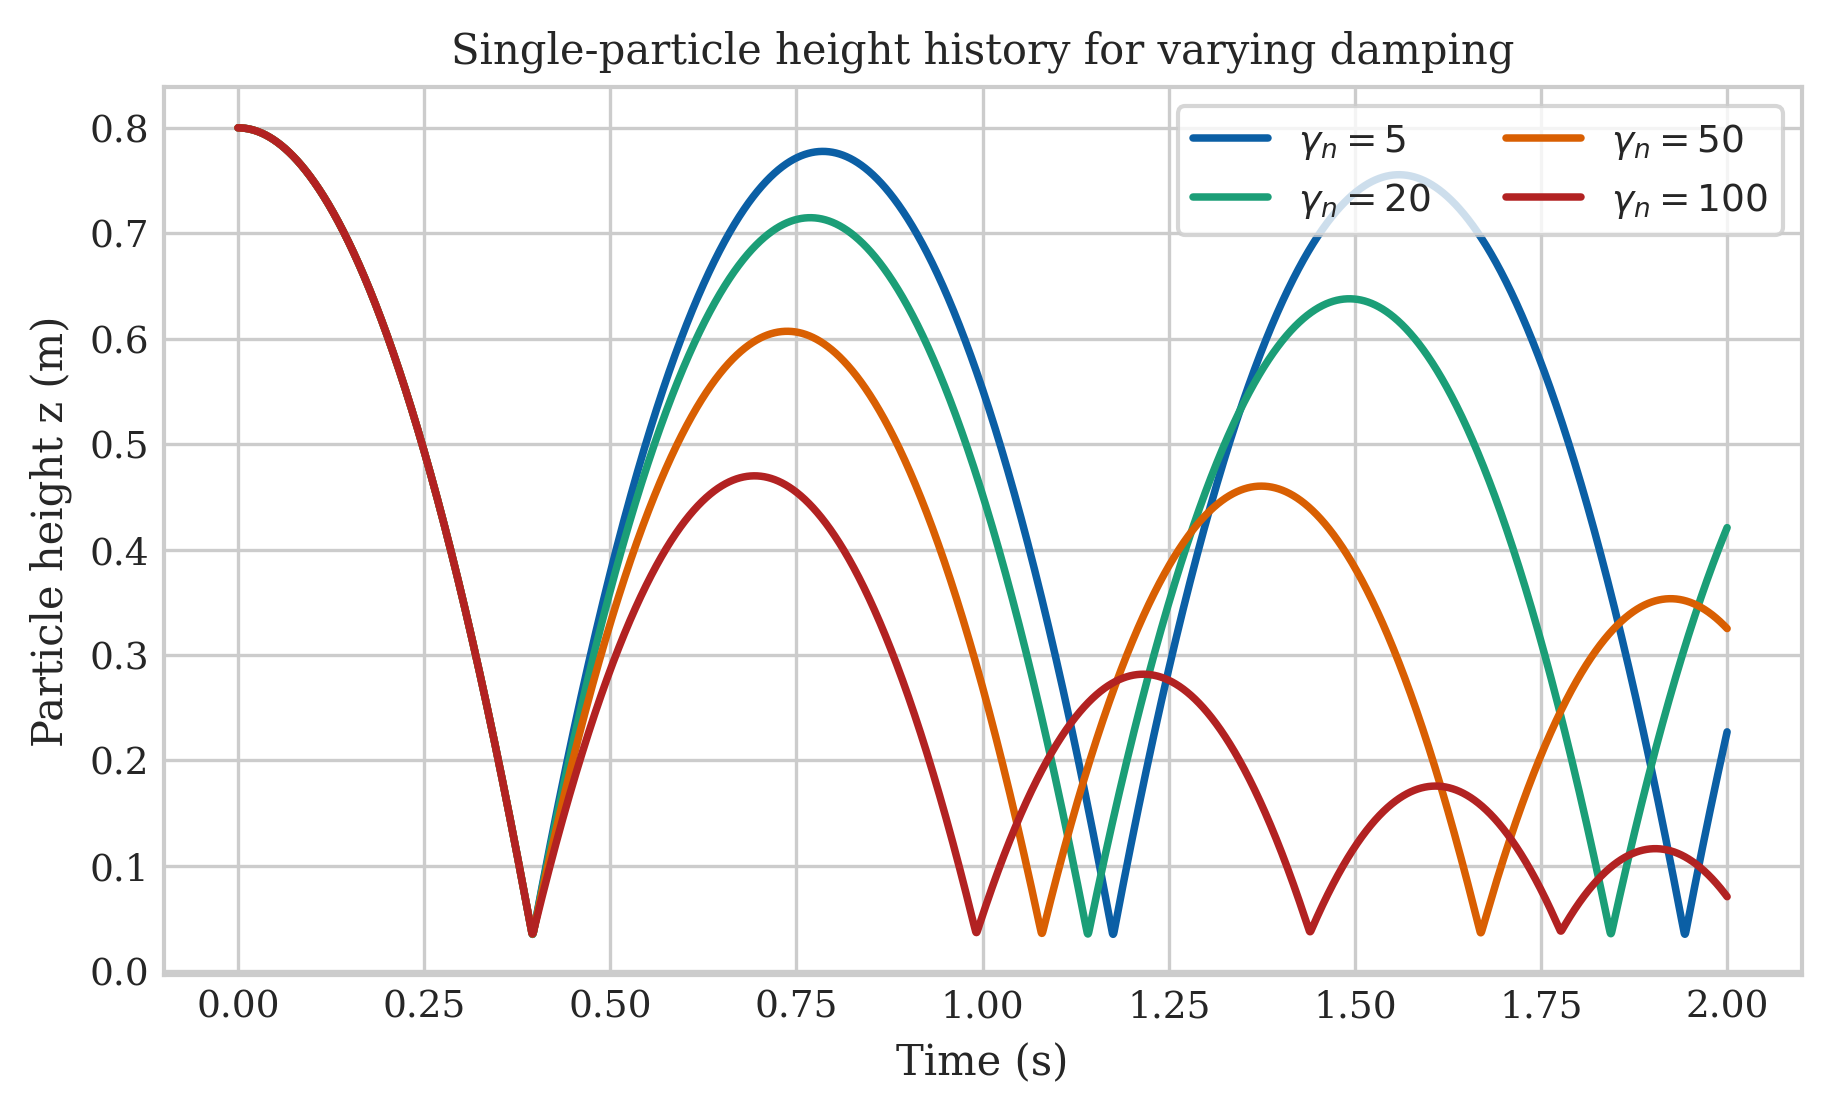
\includegraphics[width=\columnwidth]{figures/damping_height_vs_time.png}
    \caption{Single-particle height history for several damping coefficients. Larger damping reduces rebound amplitude and shortens the bouncing response.}
    \label{fig:dampingheight}
\end{figure}

Figure~\ref{fig:dampingke} shows the corresponding kinetic-energy histories. The repeated peaks correspond to free-fall acceleration between impacts, while the sharp drops occur during dissipative wall contacts. As $\gamma_n$ increases, the kinetic-energy peaks decay more rapidly from bounce to bounce, which provides a direct measure of the increased rate of energy dissipation.

This plot is useful because it separates the contact physics from the trajectory view. The height plot shows the visible response, while the kinetic-energy plot shows the mechanism behind it: stronger damping removes a larger fraction of energy at each impact, so the later peaks become much smaller and the system approaches weak motion more quickly.

\begin{figure}[t]
    \centering
    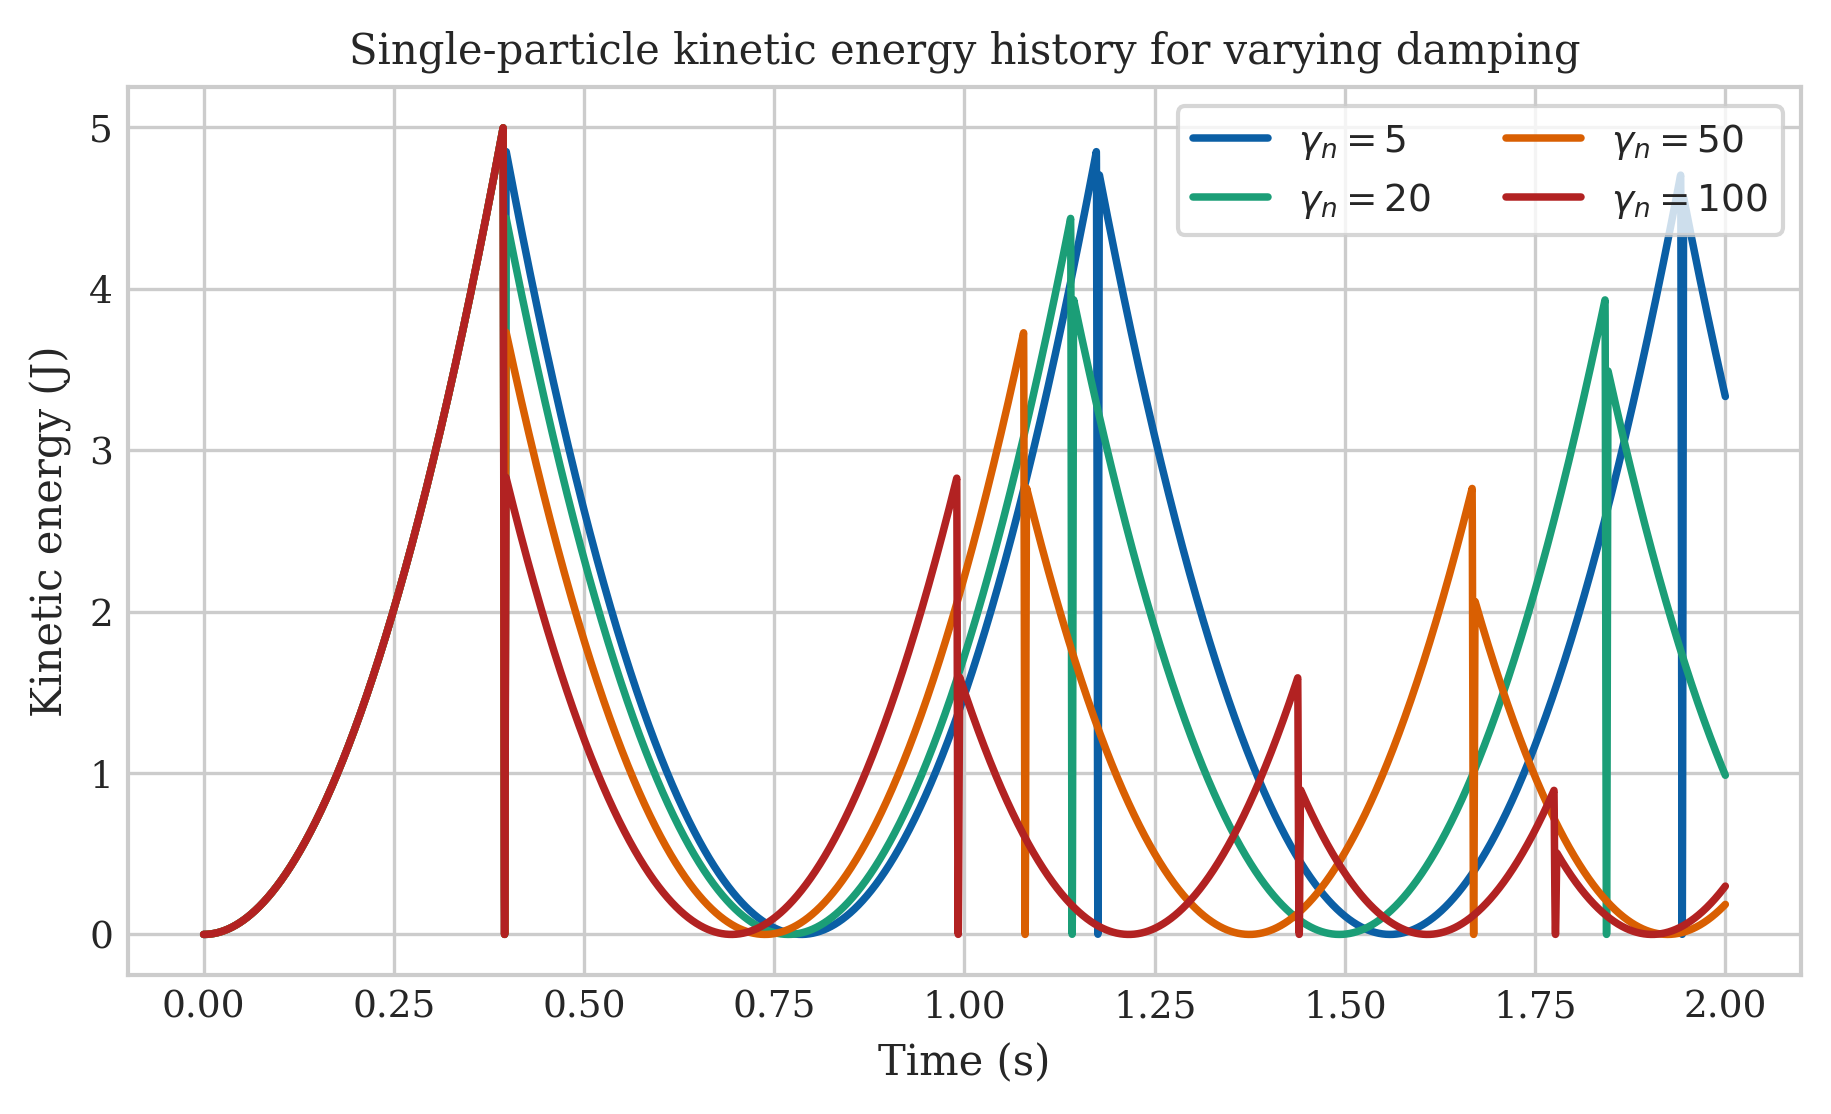
\includegraphics[width=\columnwidth]{figures/damping_ke_vs_time.png}
    \caption{Single-particle kinetic-energy history for several damping coefficients. Larger damping produces faster decay of the energy peaks after repeated impacts.}
    \label{fig:dampingke}
\end{figure}

The rebound-height analysis is summarised in Figure~\ref{fig:rebound}, which plots rebound height against bounce number. This makes the damping effect even clearer because it removes the time axis and focuses directly on the peak response after each collision. The higher-damping curves fall away more quickly, confirming that larger $\gamma_n$ leads to stronger per-impact energy loss and therefore smaller successive rebounds.

Figure~\ref{fig:damping} then combines the single-particle and particle-cloud studies in one summary view. In both systems, increasing damping lowers the remaining kinetic energy at the end of the run. The trend is clearer and more monotone in the cloud case, which suggests that repeated many-body contacts make the cumulative dissipative effect of $\gamma_n$ even more visible at the system level.

\begin{figure}[t]
    \centering
    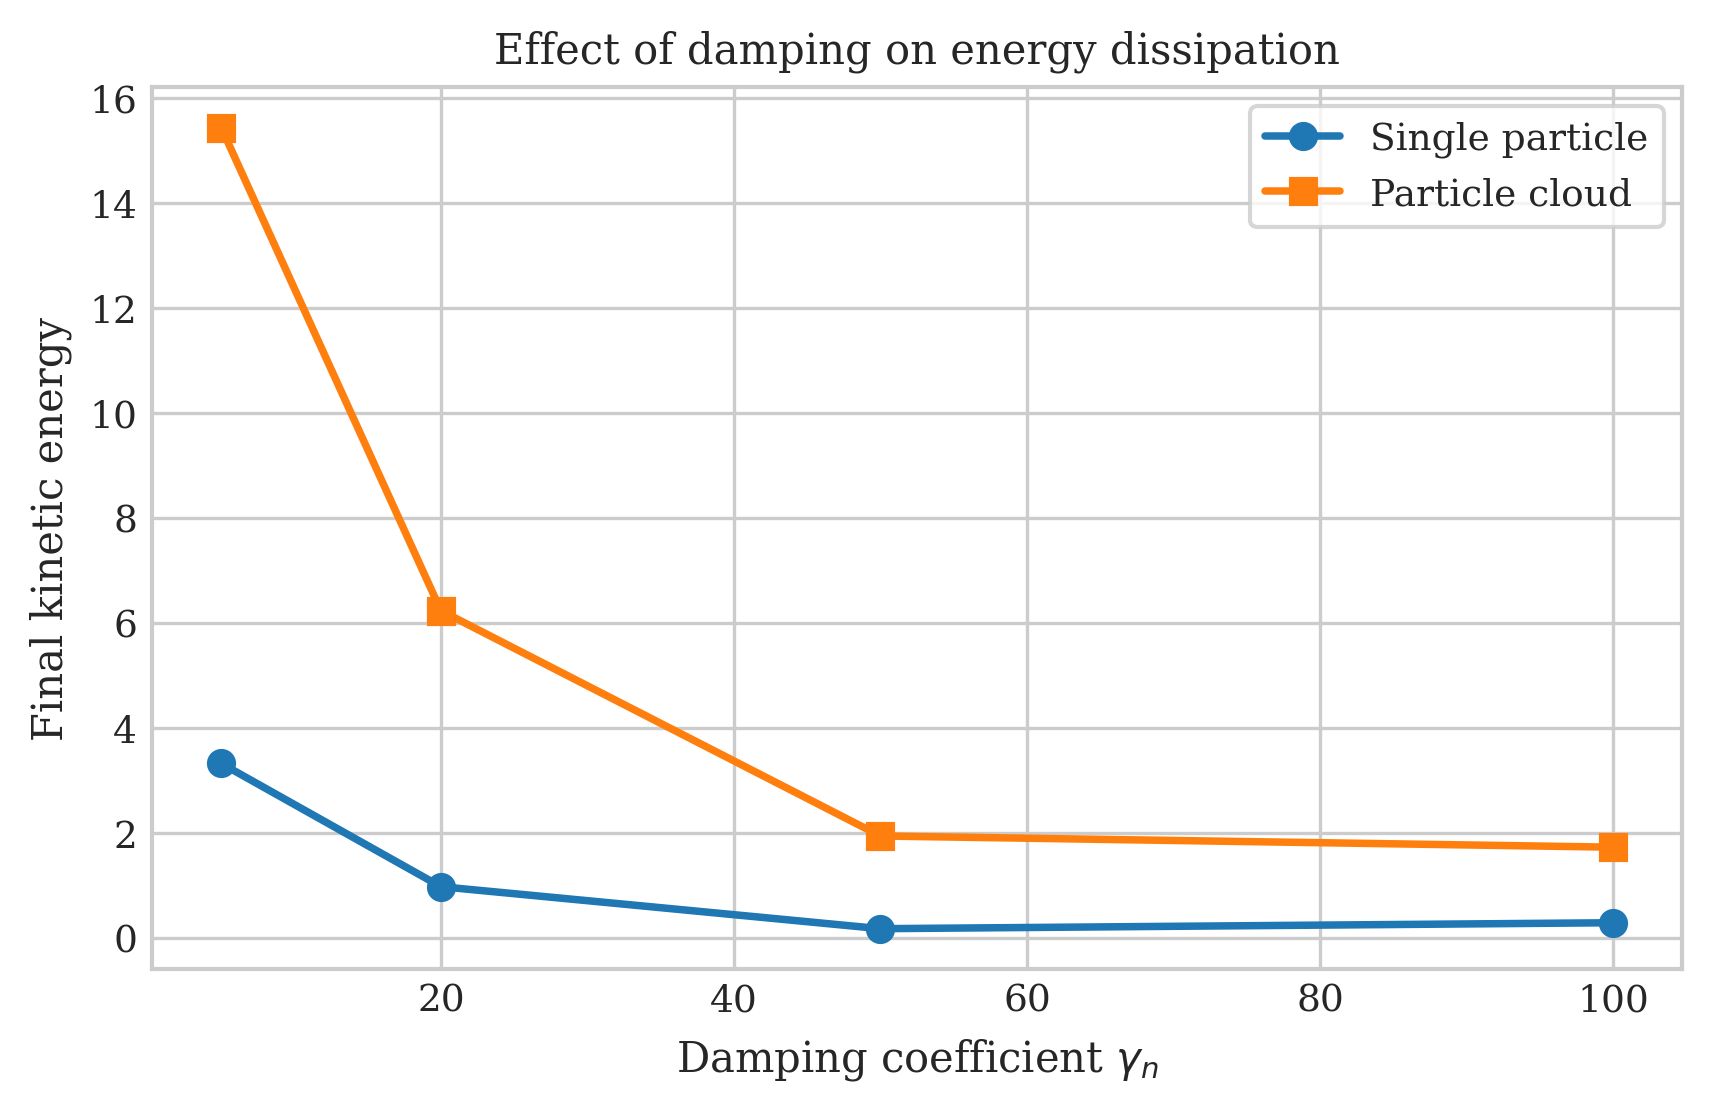
\includegraphics[width=\columnwidth]{figures/damping_vs_energy.png}
    \caption{Influence of damping on the final kinetic energy of single-particle and cloud-settling cases.}
    \label{fig:damping}
\end{figure}

\begin{figure}[t]
    \centering
    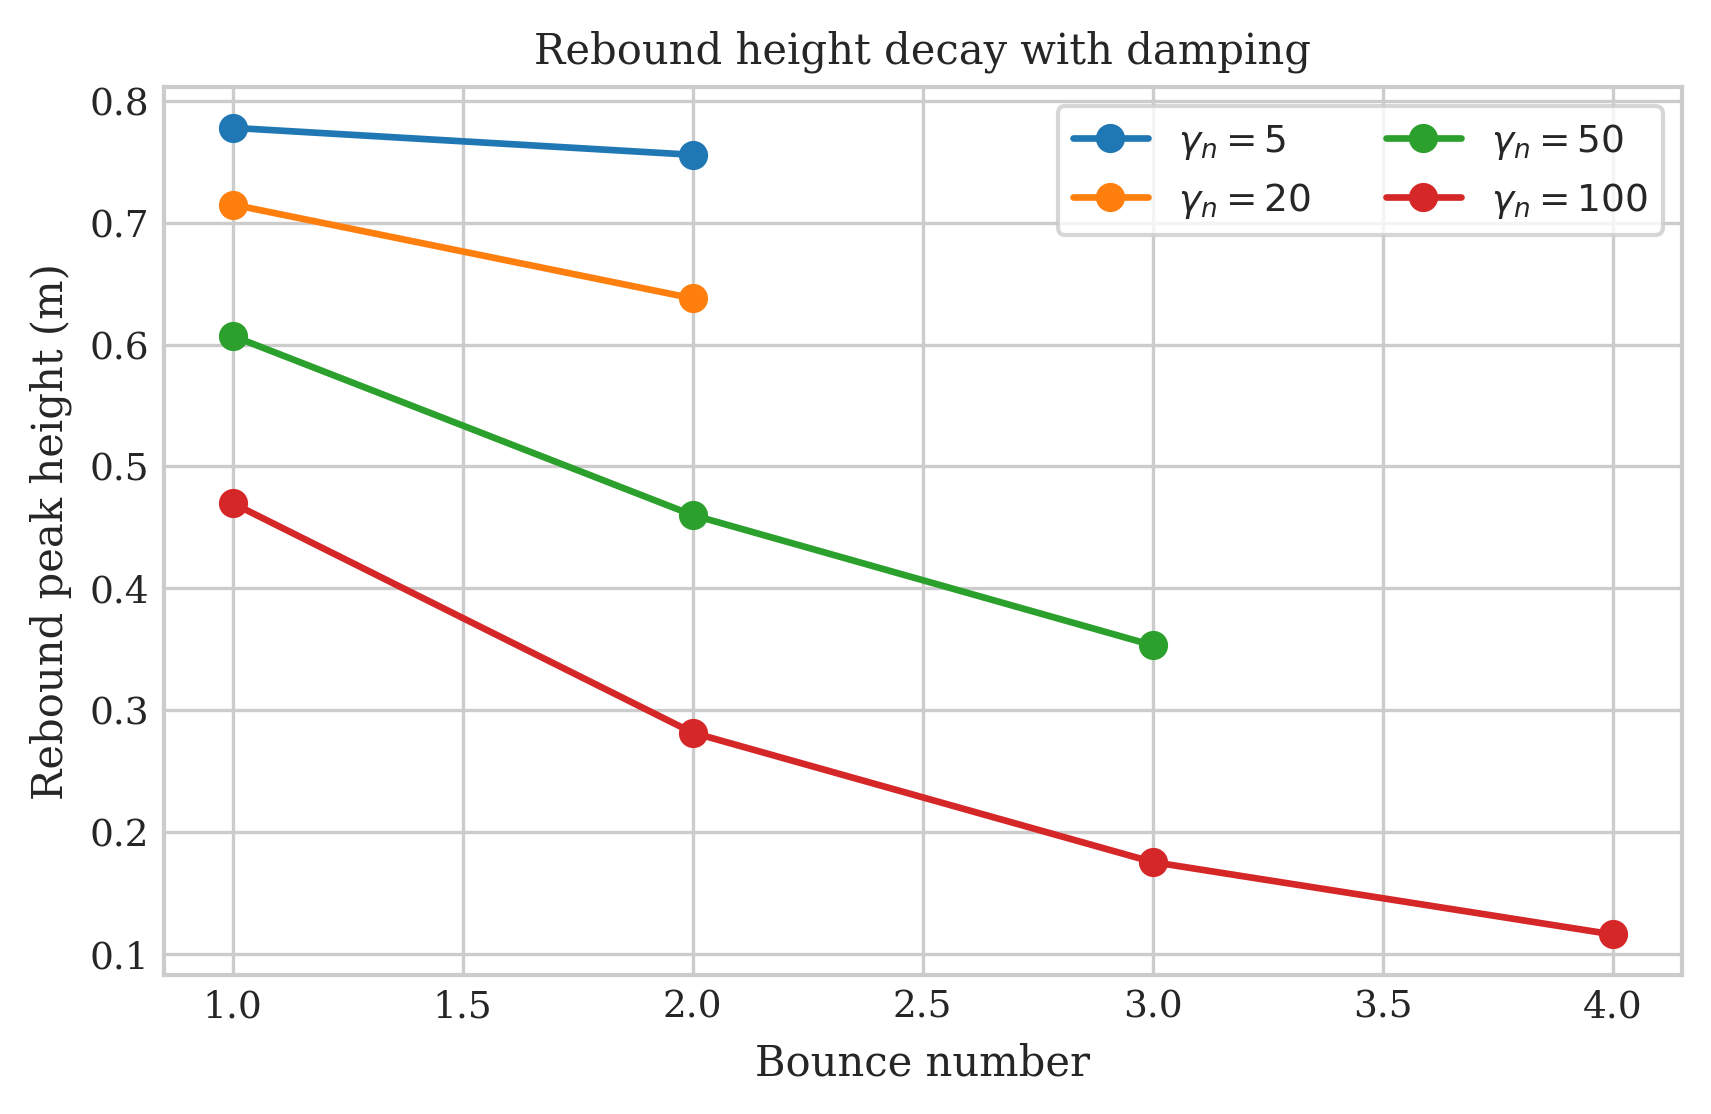
\includegraphics[width=\columnwidth]{figures/rebound_height_vs_bounce_number.png}
    \caption{Rebound peak heights for several damping coefficients.}
    \label{fig:rebound}
\end{figure}

\subsection{Particle Cloud Settling}
For the cloud-settling study, a collection of particles was initialised in the box with zero initial velocity and then allowed to settle under gravity. This setup follows the assignment statement directly and provides a simple many-particle test of emergent behaviour. The evolution was analysed using the center-of-mass height, the total kinetic energy, and particle configurations at selected times.

Figure~\ref{fig:clouddiag} shows the time evolution of the center-of-mass height and total kinetic energy for the settling cloud. The center of mass drops steadily as the particles rearrange under gravity, while the kinetic energy rises initially as gravitational potential energy is converted into motion and then fluctuates as contacts redistribute and dissipate that motion. These two diagnostics together give a compact view of the global settling process: downward migration of the cloud and simultaneous contact-driven energy redistribution.

The combination of these two curves is important for interpretation. The center-of-mass height gives the bulk settling trend, whereas the kinetic-energy history shows that the settling is not purely smooth drift: it is mediated by repeated collisions, short bursts of rearrangement, and dissipation. In other words, the cloud settles collectively through many local contact events rather than through independent particle motion.

\begin{figure}[t]
    \centering
    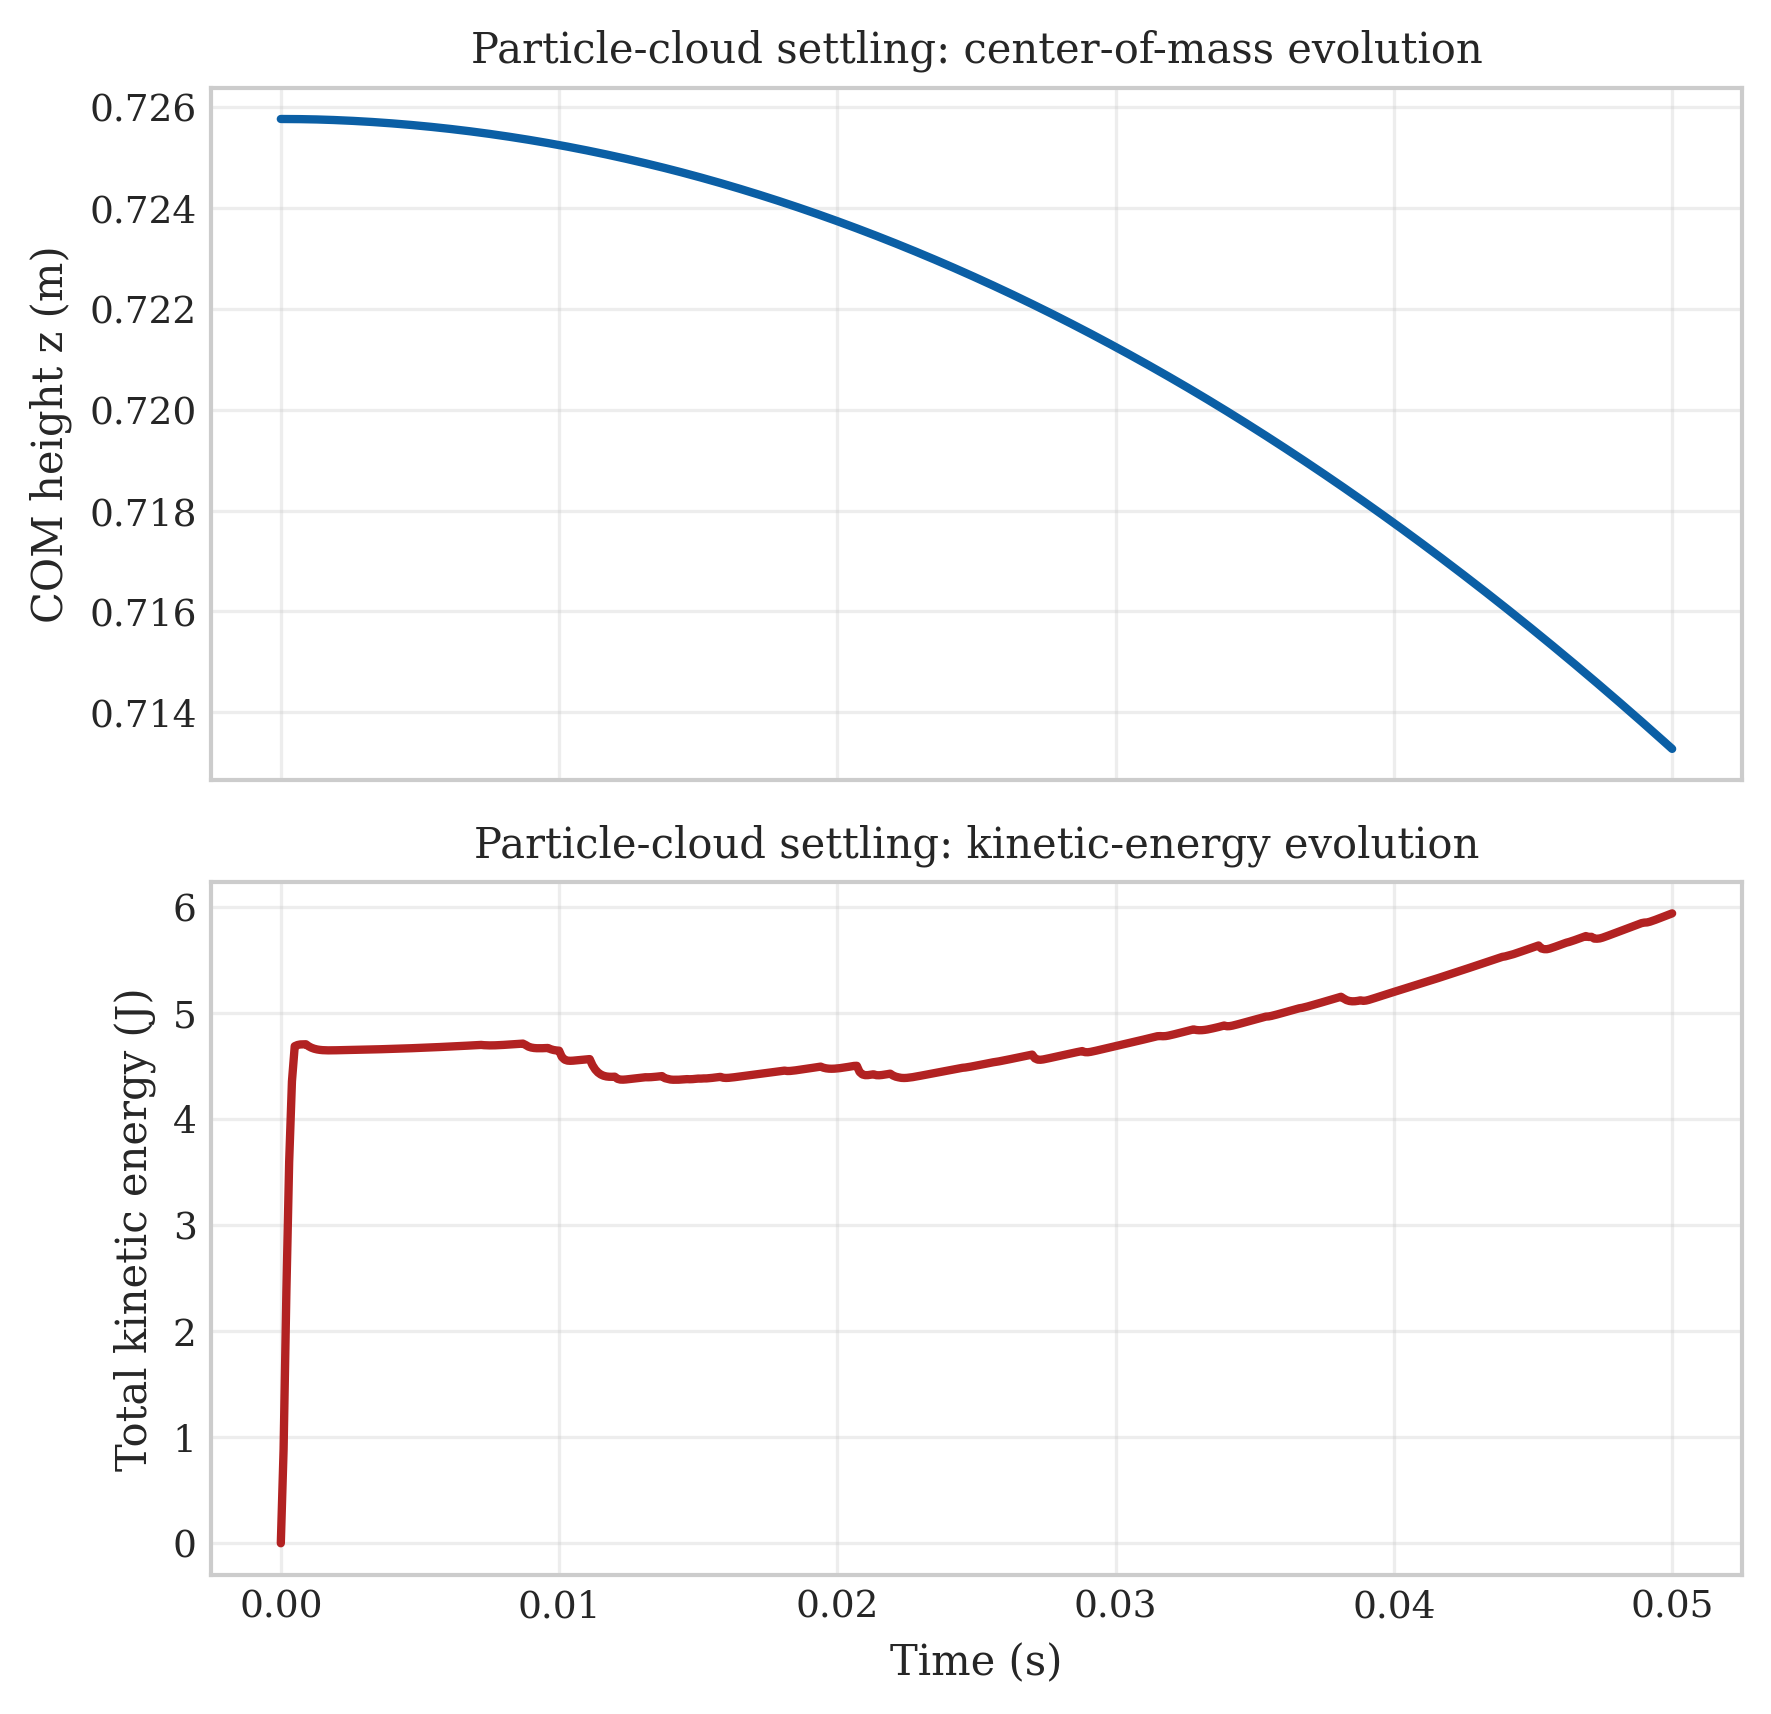
\includegraphics[width=\columnwidth]{figures/cloud_settling_diagnostics.png}
    \caption{Particle-cloud settling diagnostics showing center-of-mass height and total kinetic energy as functions of time.}
    \label{fig:clouddiag}
\end{figure}

Figure~\ref{fig:cloudconfigs} shows particle configurations at selected times during the same run. The sequence illustrates the emergent system behaviour visually: the initially suspended cloud compacts downward, collisions spread momentum through the packing, and the particles progressively form a denser lower-region structure as settling proceeds.

These configuration snapshots are helpful because they connect the scalar diagnostics to the actual geometry of the particle assembly. The decreasing center-of-mass height and changing kinetic energy are therefore not only abstract numbers; they correspond to visible compaction, rearrangement, and the gradual formation of a settled particle bed near the bottom of the box.

\begin{figure}[t]
    \centering
    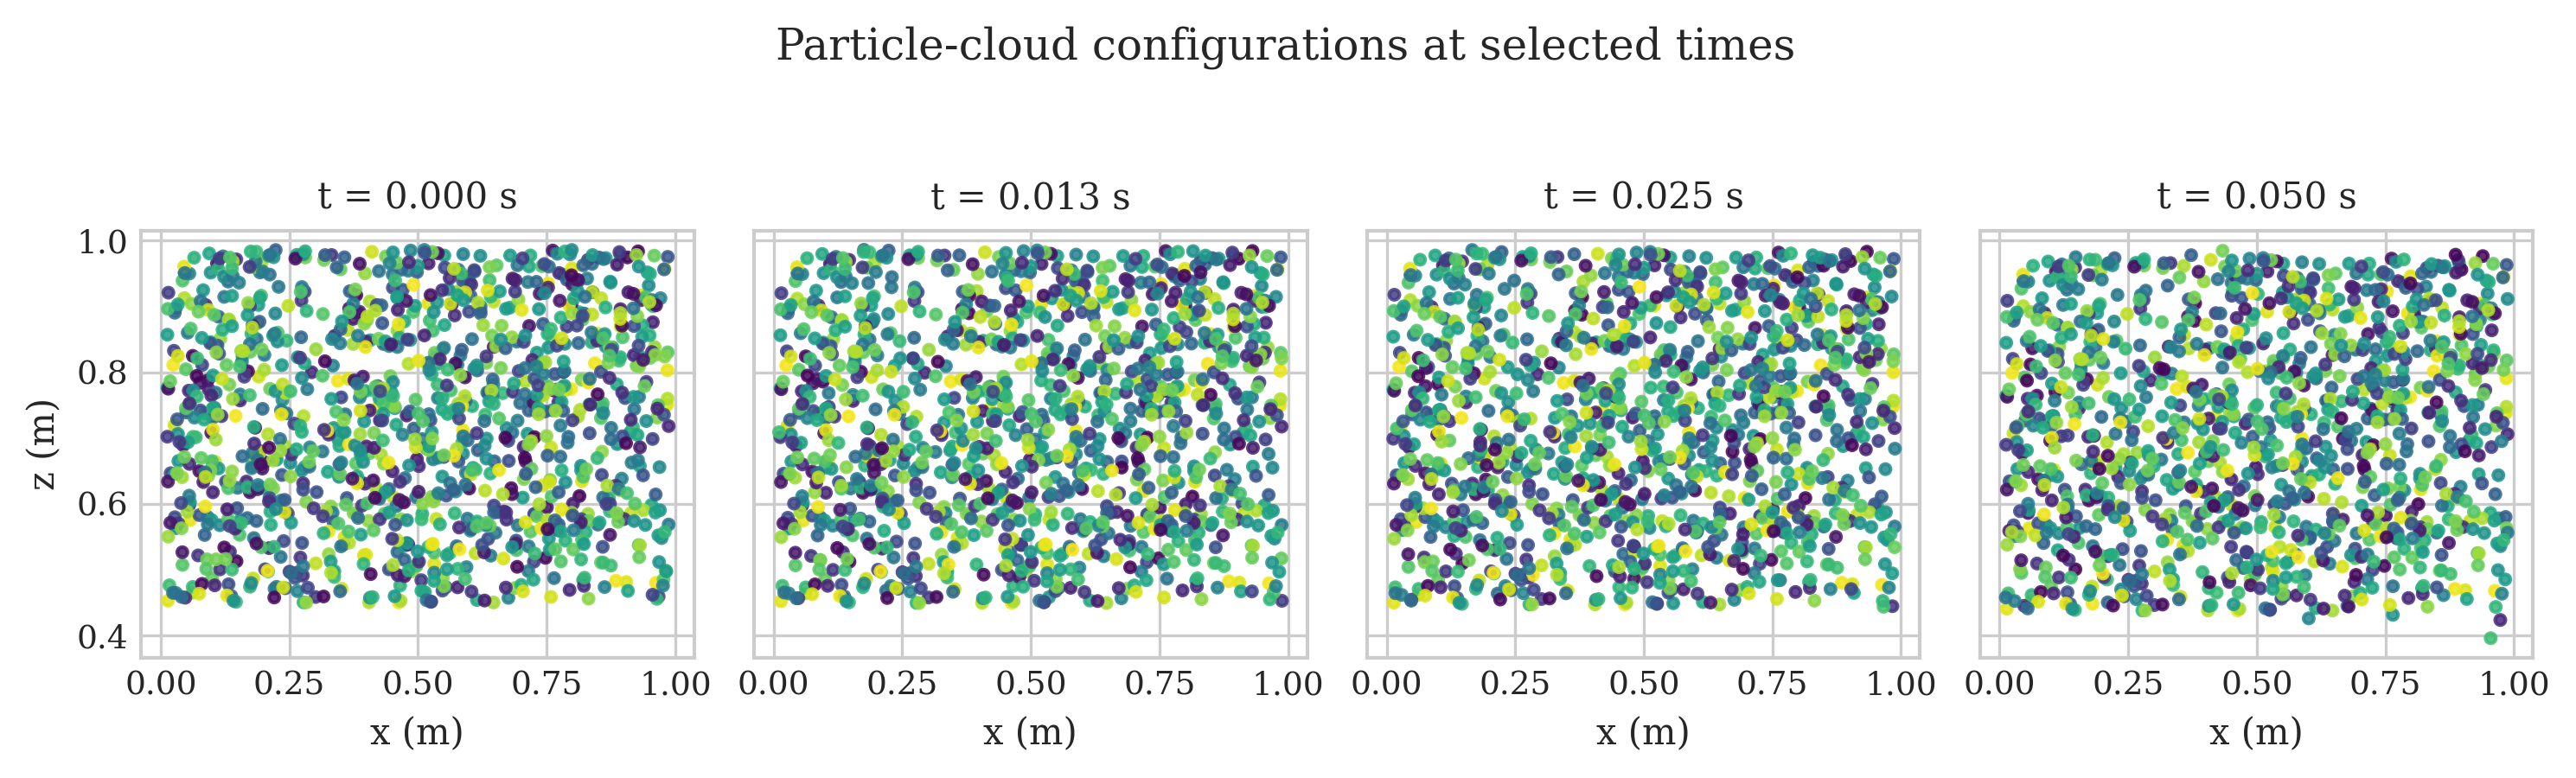
\includegraphics[width=\columnwidth]{figures/cloud_settling_configurations.png}
    \caption{Particle-cloud configurations at selected times during the settling process.}
    \label{fig:cloudconfigs}
\end{figure}

The cloud-settling study was then repeated for different damping coefficients so that the emergent behaviour could also be examined as a function of $\gamma_n$. Figure~\ref{fig:clouddamping} shows that increasing the damping coefficient reduces the final kinetic energy of the particle cloud and slightly changes the final center-of-mass height. The reduction in final kinetic energy is the clearest trend: stronger damping suppresses residual collective motion and drives the system toward a more strongly dissipated settled state.

The variation in final center-of-mass height is smaller than the variation in final kinetic energy, which is also physically reasonable. The damping coefficient mainly changes how motion is dissipated during collisions; it has a stronger effect on how energetic the cloud remains than on the final gross position of the settled mass over this short simulation window.

\begin{figure}[t]
    \centering
    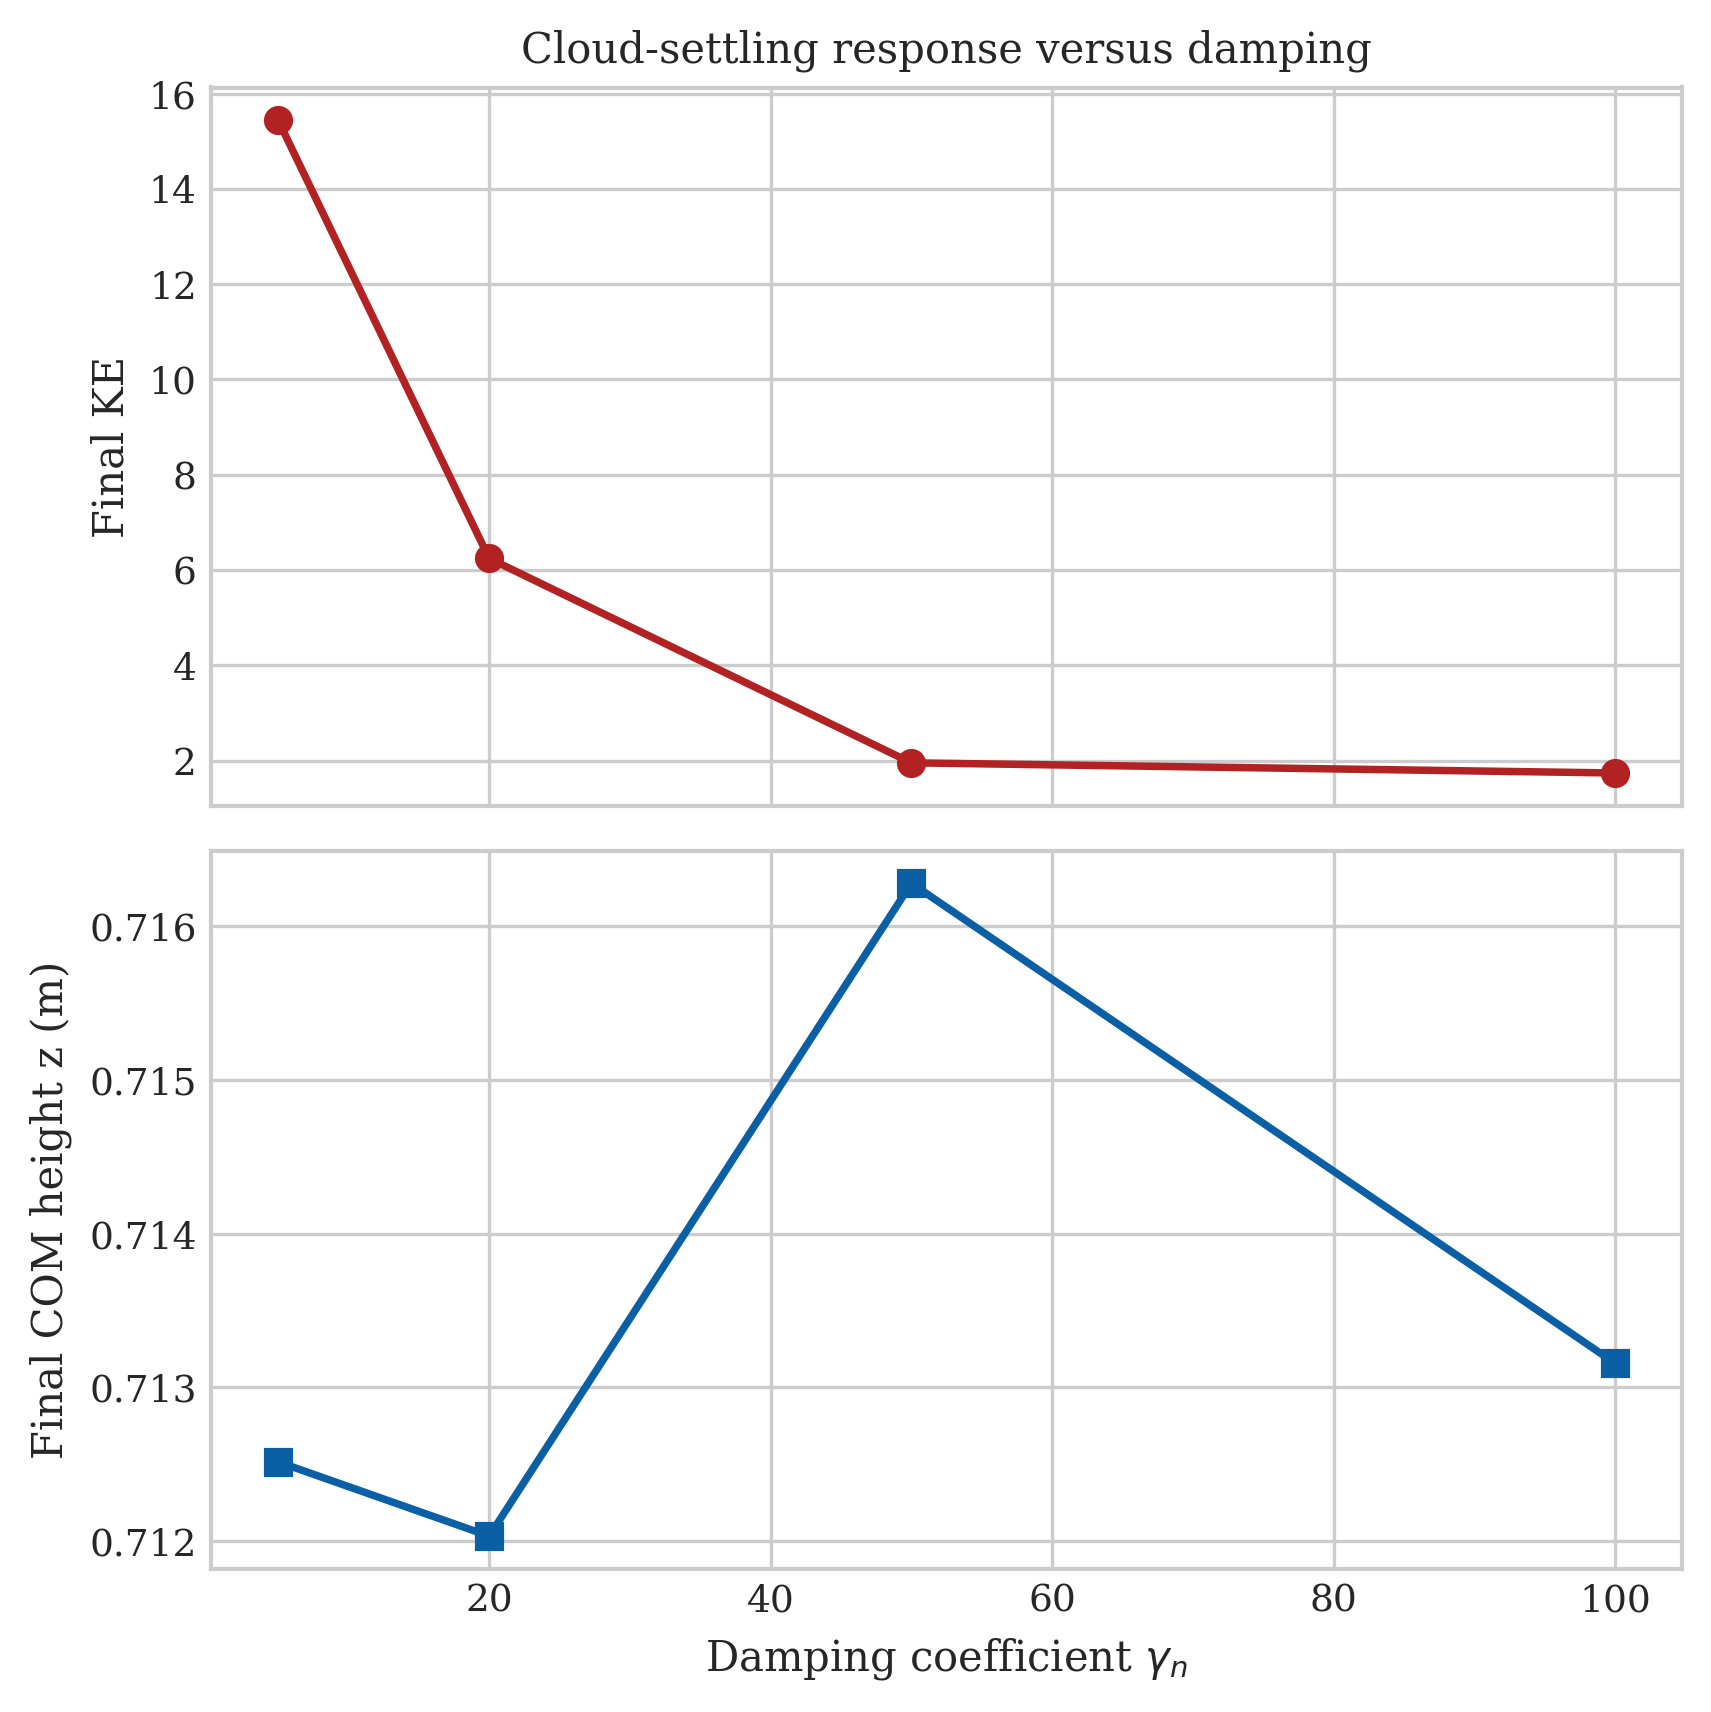
\includegraphics[width=\columnwidth]{figures/cloud_damping_response.png}
    \caption{Dependence of particle-cloud settling outcomes on damping coefficient. Larger damping reduces the final kinetic energy and slightly modifies the final center-of-mass height.}
    \label{fig:clouddamping}
\end{figure}

These cloud results complement the one-particle bounce study. The single-particle plots explain the local contact physics clearly: larger damping reduces rebound height and increases the rate of energy loss after repeated floor impacts. The cloud-settling results then show how the same contact-level dissipation appears at the collective level, where stronger damping reduces residual motion, weakens post-collision agitation, and promotes a more rapidly damped emergent particle arrangement. In summary, the damping study and the cloud-settling study together show that the dashpot coefficient controls both the local rebound response of individual contacts and the large-scale emergent behaviour of the many-particle system.

\begin{figure}[t]
    \centering
    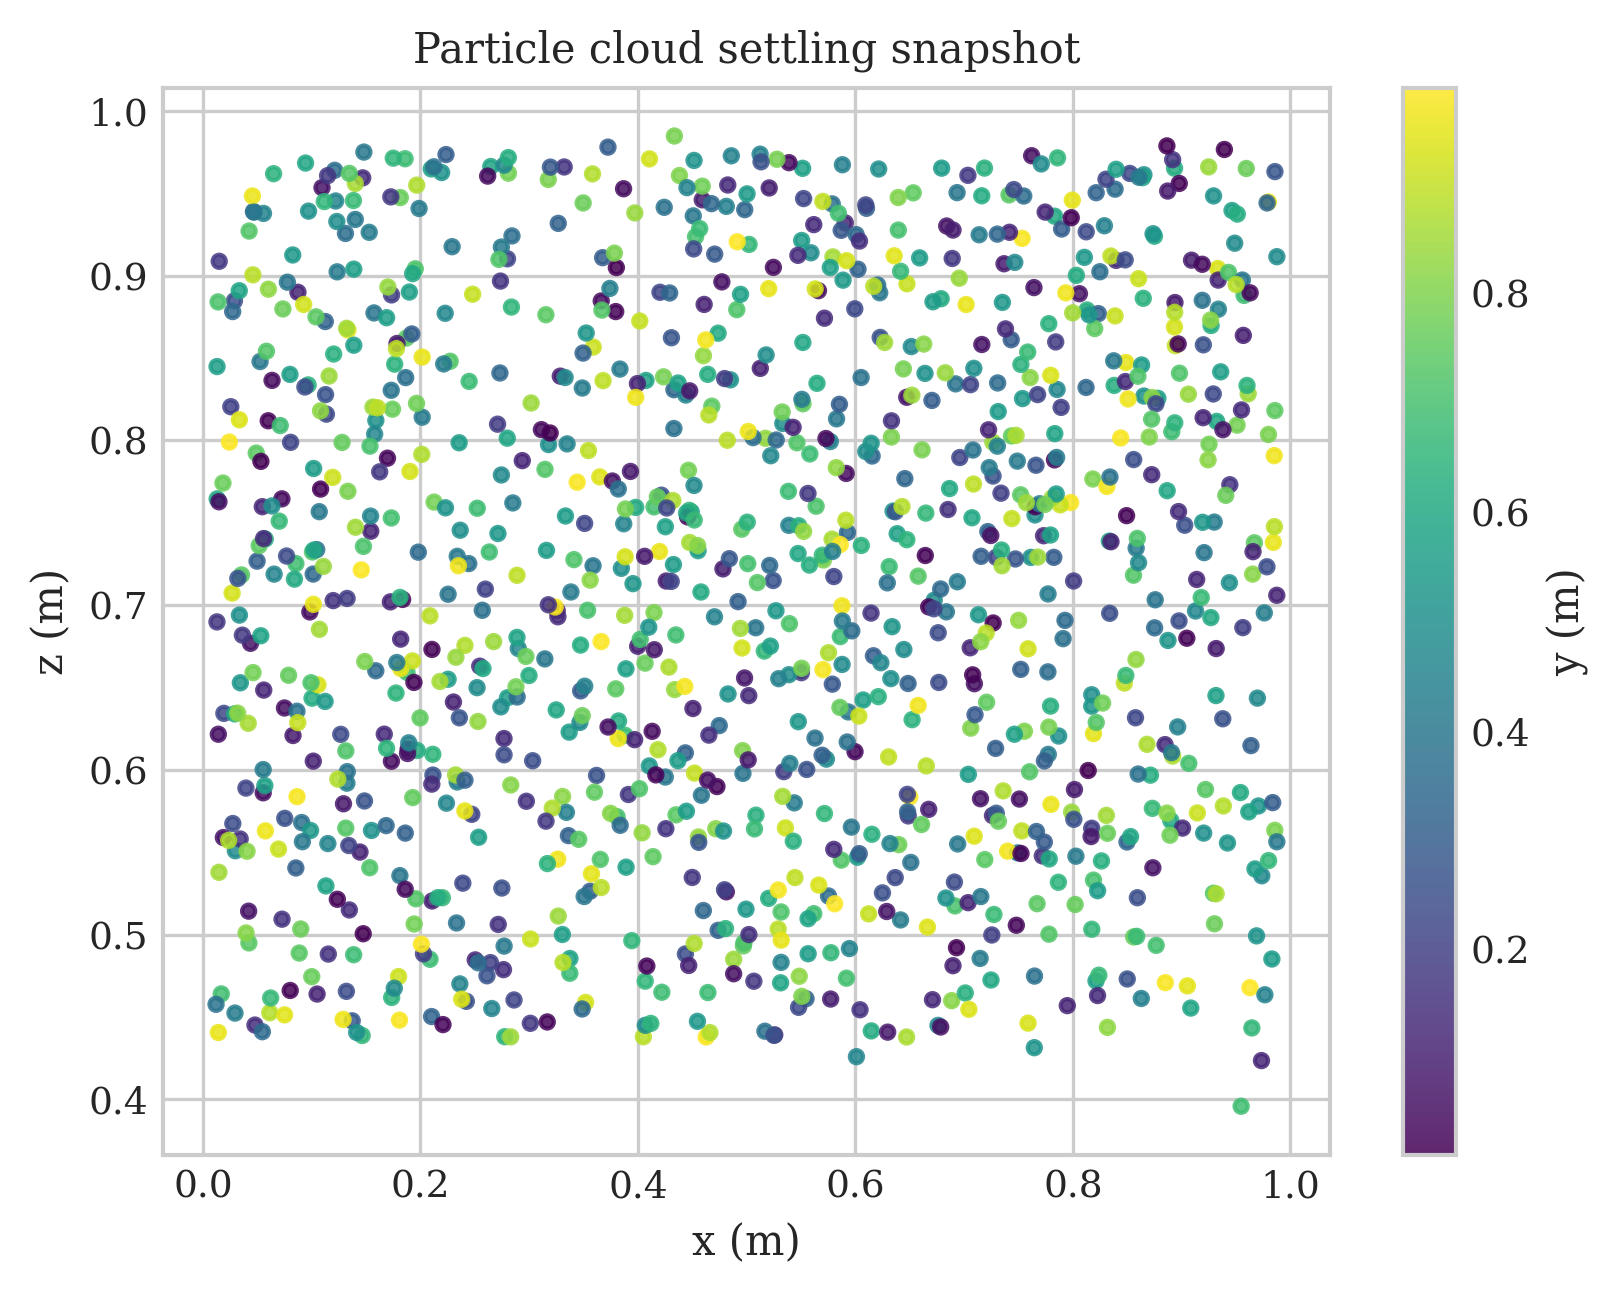
\includegraphics[width=\columnwidth]{figures/cloud_settling_snapshot.png}
    \caption{Representative particle-cloud settling snapshot in the $x$-$z$ plane.}
    \label{fig:cloud}
\end{figure}

\section{Discussion and Conclusions}
This paper presented a complete workflow for a simple three-dimensional DEM solver: physical formulation, numerical implementation, verification, profiling, OpenMP parallelisation, neighbour search, and two bonus scientific studies. The verification cases showed that the solver reproduces the expected free-fall, constant-velocity, and bounce behaviour. The profiling and scaling studies then identified the particle-contact loop as the dominant bottleneck and showed that OpenMP provides useful acceleration, especially for the larger particle-count cases.

The additional studies in the paper support the same overall picture. The neighbour-search method preserved detected-contact correctness while reducing candidate pairs and runtime strongly for the larger systems, although its overhead was not worthwhile for the smallest test case. The damping and cloud-settling studies showed that changing the damping coefficient affects both the local rebound response of single-particle impacts and the emergent collective behaviour of many-particle settling.

In conclusion, the work completed in this paper demonstrates that even a compact DEM solver can be verified carefully, analysed quantitatively, and improved both computationally and physically. The final code remains a simplified baseline model with translational motion and normal contact forces only, but within that scope it successfully reproduces the behaviours and performance trends studied in the report.

\section*{Code and Reproducibility}
Source code, build instructions, and scripts are included in the project repository. The main solver is in \texttt{src/main.cpp}, the plotting script is in \texttt{scripts/plot\_results.py}, and generated figures are stored in \texttt{report/figures}. CSV outputs were used for all plots in this paper.

\section*{Use of LLM Assistance}
An LLM-based coding assistant was used during development for code drafting, cleanup, and report structuring. All generated material was manually reviewed, edited, compiled, and checked against the assignment requirements before inclusion in the final submission.

\end{document}
